\documentclass{bmstu}
\usepackage{pdfpages}

\def\labelitemi{---}

\bibliography{biblio}

\begin{document}
	
    \makecourseworktitle
    {Информатика и системы управления} % Название факультета
    {Программное обеспечение ЭВМ и информационные технологии} % Название кафедры
    {Разработка базы данных для IoT-платформы умный дом} % Тема работы
    {Мамврийский~И.~С./ИУ7-66Б} % Номер группы/ФИО студента (если авторов несколько, их необходимо разделить запятой)
    {Гаврилова~Ю.~М.} % ФИО научного руководителя
    {} % ФИО консультанта (необязательный аргумент; если консультантов несколько, их необходимо разделить запятой)

    \setcounter{page}{3}
    \chapter*{РЕФЕРАТ}

Целью курсовой работы является разработка базы данных для IoT-платформы умный дом, а так же создание Web–приложения для взаимодействия с данными.

Расчетно–пояснительная записка содержит 43 страницы, 4 таблицы, 28 иллюстраций, 19 источников.

Ключевые слова: IoT-система, умный дом, статус устройства, многопользовательский доступ, владелец, чистая архитектура, GoLang, база данных, система управления базой данных, PostgreSQL.

    \maketableofcontents
    
    \chapter*{Введение}

В настоящее время технологии интернета вещей (IoT) становятся 
неотъемлемой частью нашей повседневной жизни, и одним из наиболее 
заметных примеров их применения является IoT-платформа для умного дома. 
Она объединяет различные устройства в доме, от 
светильников до умных термостатов, в единую сеть, которая может 
управляться и контролироваться через интернет.

Основной целью IoT-платформы умного дома является создание 
интеллектуальной инфраструктуры, способной адаптироваться к 
потребностям и предпочтениям пользователей. Она обеспечивает 
возможность контролировать освещение, отопление, кондиционирование 
воздуха, безопасность и другие аспекты жизни в доме с помощью смартфона 
или другого устройства с доступом в интернет.

С учетом быстрого развития технологий IoT и роста спроса на умные 
системы, платформы умного дома становятся все более интегрированными, 
расширяя свои возможности и предлагая новые функции для улучшения 
качества жизни пользователей.

Целью курсовой работы является разработка базы данных для IoT-платформы умный дом. 
Для достижения поставленной цели необходимо выполнить следующие задачи:
\begin{enumerate}
    \item провести анализ существующих решений;
    \item сформулировать требования к разрабатываемой базе данных;
    \item проанализировать существующие базы данных на основе данной задачи;
    \item спроектировать и разработать базу данных;
    \item спроектировать и разработать приложение для взаимодействия с базой данных;
    \item провести исследование зависимости времени выполнения запросов
    с использованием индексов и без.
\end{enumerate}

	\chapter{Аналитическая часть}

\section{Существующие решения}

Так как IoT-вещей активно развиваются, то на рынке уже представлены различные платформы умных домов. 
Рассмотрим наиболее популярные из них:
\begin{itemize}
    \item Apple Homekit
    \item Intel IoT Platform
    \item MTS IoT HUB
    \item Xiaomi MI
\end{itemize}

Выделим следующие критерии для сравнения выбранных платформ:
\begin{enumerate}
    \item[1)] Многопользовательский доступ
    \item[2)] Возможность создания нескольких домов
    \item[3)] История работы устройств
\end{enumerate}

Сравнение выбранных платформ по указанным критериям представлены в таблице \ref{tab:solutions}:
\begin{table}[!ht]
    \centering
    \caption{\label{tab:solutions} Сравнение существующих решений}
    \begin{tabular}{|l|l|l|l|l|l|}
    \hline
        Решение & 1 & 2 & 3  \\ \hline
        Apple Homekit & + & + & - \\ \hline
        Intel IoT Platform & - & - & + \\ \hline
        MTS IoT HUB & - & + & + \\ \hline
        Предполагаемое решение & + & + & + \\ \hline
    \end{tabular}
\end{table}

Таким образом, ни одна из плафторм не удовлетворяет всем критериям. 

\section{Формулирвока требований к разрабатываемой базе данных и приложению}

В ходе выполнения курсовой работы необходимо разработать базу данных для хранения ифнормации 
о пользователях, умных домах, устройствах. 

Помимо этого, нужно спроектировать Web-приложение, 
которое будет предоставлять интерфейс для взаимодействия с базой данных с возможностью создавать умные дома, 
добавлять новые устройтва в свой дом, просматривать историю работы устройств.
    
Необходимо также предусмотреть многопользовательский доступ к дому, возможность добавления других пользователь 
в свой дом для совместного управления. Требуется реализовать функциональность для разных категорий пользователей, 
каждый из которых получает свой определенный набор прав.

\section{Формализация xданных}

Разрабатываемая база данных для IoT платформы умного дома должна содержать информаицю о пользователях, устройствах, умных домах,
истории работы устройств. Данные категории показаны на ER-диаграмме в нотации Чена \ref{img:er}.

\begin{figure}[h]
    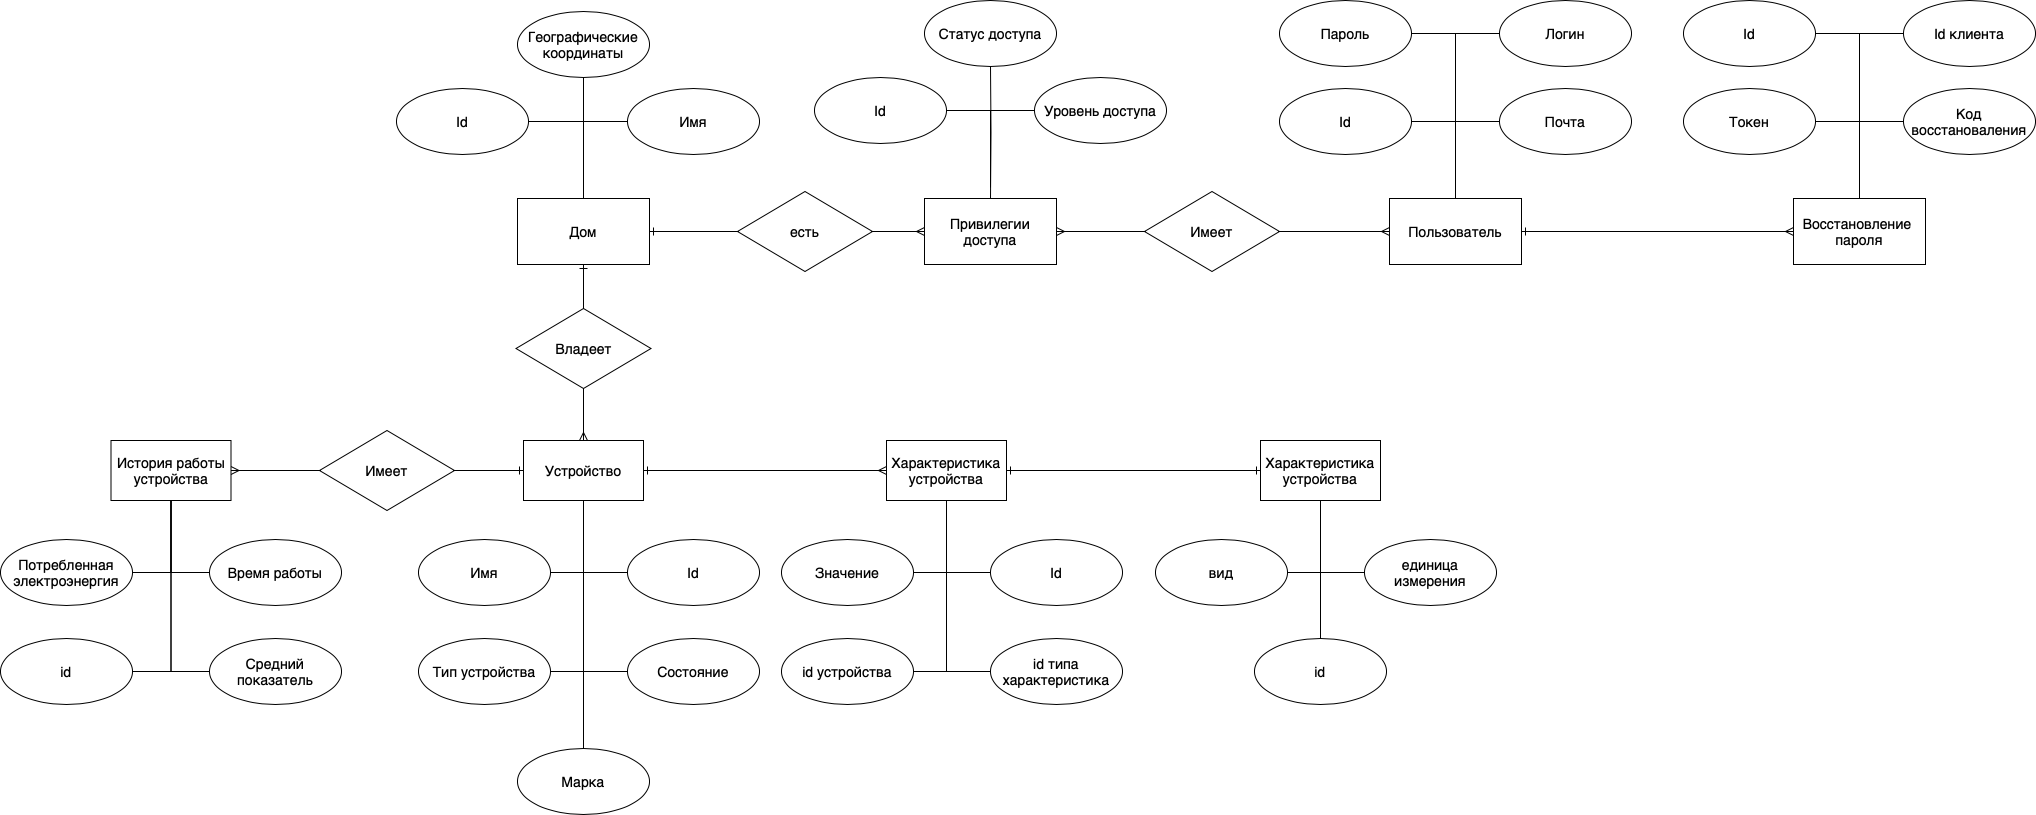
\includegraphics[width=0.9\linewidth]{img/er.png}
    \caption{ER-диаграмма в нотации Чена}
    \label{img:er}
\end{figure}
\noindent
\clearpage

\section{Анализ существующих баз данных на основе формализации задачи}
База данных -- \textbf{самодокументированное} собрание \textbf{нтегрированных} записей. Рассмотрим части данное определения:
\begin{enumerate}
    \item База данных является самодокументированной, то есть содержит описание собственной струкутры, которое называется 
    словарем данных, каталогом данных или метаданными.
    \item База данных -- собрание интегрированных записей, она содержит:
    \begin{itemize}
        \item файлы данных,
        \item метаданные,
        \item индексы,
        \item может содеражтьетаданные приложений.
    \end{itemize}
    \item База данных является информационной моделью пользовательской модели предметной области.
\end{enumerate}

% Добавить автора Кренке, Теория и практика построения БД 2003

Модель базы данных определяет логическую структуру базы данных и то, каким образом данные будут храниться, организовываться
и обрабатываться.

Существует три основных типа моделей базы данных:
\begin{itemize}
    \item дореляционные;
    \item реляционные;
    \item постреляционные.
\end{itemize}

\subsection{Дореляционная база данных}

К дореляционным моделям баз данных относятся иерархическая и сетевая модели.

Иерархическая модель состоит из объектов с указателями от родительских объектов к потомкам, 
соединяя вместе связанную информацию. Она может быть представлена в виде дерева. Одним из больших минусов данной
модели является невозможность отношения "многие-ко-многим"

Основными понятиями сетевой модели базы данных являюся узел и связь. Узел -- совокупность атрибутов данных, описывающих
некоторый объект. Данная база данных может быть предствлена в виде графа. При изменении структуры данной модели придется 
изменять и приложние, так как логика процедуры выборки данных зависит от физической организации этих данных.

\subsection{Реляционная база данных}
В реляционных моделях данные организованы в набор двумерных взаимосвязанных таблиц. 
Каждая из которых представляет собой набор столбцов и строк, где столбец представляет атрибуты сущности, 
а строки представляют записи. Такое представление обеспечивает простой и эффективный способ хранения структурированной информации, 
доступа к ней, а также легкую сортировку.

Также в данной модели происходит разделение между физическим и логическим уровнями, что 
позволяет управлять физической системой хранения, не меняя данных, содержащихся в логической структуре.

% ToDo https://www.oracle.com/cis/database/what-is-a-relational-database/

\subsection{Постреляционные}

Нереляционная база данных —- это база данных, в которой в отличие от большинства традиционных систем баз данных 
не используется табличная схема строк и столбцов. В этих базах данных применяется модель хранения, оптимизированная 
под конкретные требования типа хранимых данных. Например, данные могут храниться как простые пары "ключ — значение", 
документы JSON или граф, состоящий из ребер и вершин. Все эти хранилища данных не используют реляционную модель. 

% ToDo https://learn.microsoft.com/ru-ru/azure/architecture/data-guide/big-data/non-relational-data

Недостатком такой модели является сложность решения проблемы обеспечения целостности и непротиворечивости хранимых данных.


\section{Формализация и описание пользователей проектируемого приложения к базе данных}
Для взаимодействия с Web-приложением было выделено четыре категории пользователя: новый пользователь,
владелец, участник дома, зарегистрированный пользователь.

Все возможные функции для каждой категории пользователей представлены на следующей Use-case диаграмме \ref{img:iot}
\begin{figure}[h]
    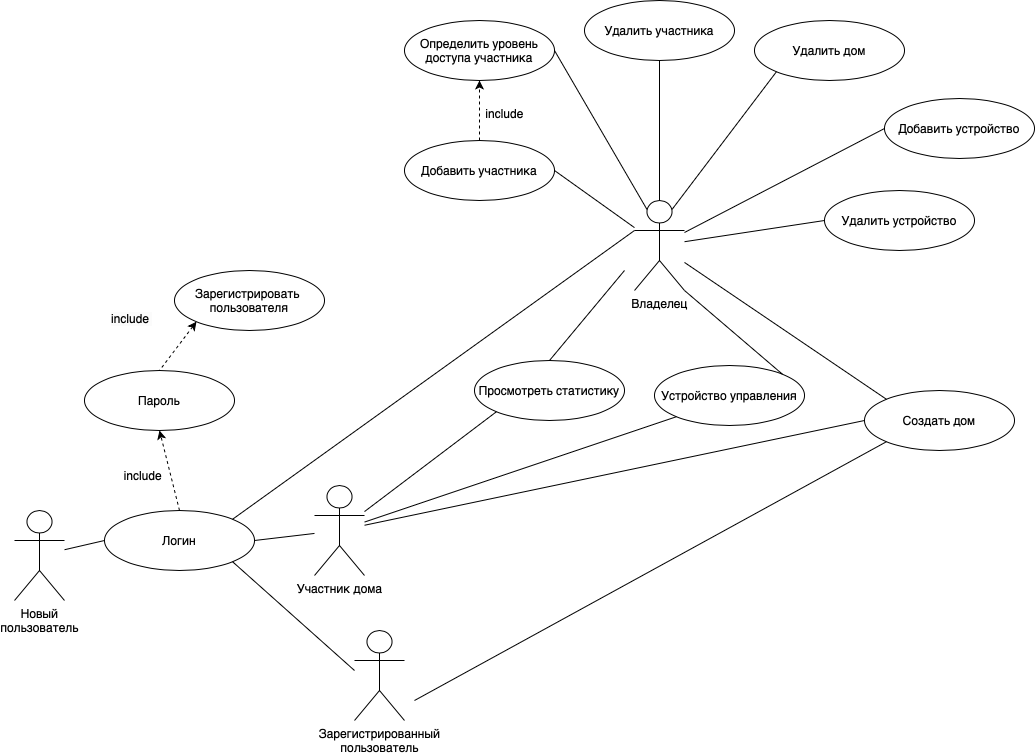
\includegraphics[width=0.9\linewidth]{img/iot.png}
    \caption{Use-case диаграмм полльзователей}
    \label{img:iot}
\end{figure}
\noindent

Новый пользователь -- незарегистрированный пользователь, который получает возможность зарегистрироваться 
на IoT платформе, введя логин и пароль. 

Зарегистрированный пользователь -- пользователь, который прошел регистрацию. Он может создать собственный дом или стать участником 
дома.

Участник дома - пользователь, который который вступил в дом. В зависимостьи от уровня доступа ему доступны следующие функции:
просмотр статистики, управление устройствами, также при необходимости он может создать собственный дом.

Владелец -- пользователь, который создал дом. Ему доступен наибольший функционал, помимо функций доступных участнику,
он может добавлять/удалять участников дома, устройства, определять уровень доступа других участников к дому. Также владелец 
может стать участником другого дома.

\section*{Вывод}

В данном разделе проведен анализ аналогов IoT-платформ для умного дома.
Ни одно из исследованных решений не соответствовало всем установленным критериям сравнения. 
При рассмотрении моделей баз данных было принято решение в пользу реляционной модели. 
Это обосновано необходимостью обеспечения целостности хранящихся данных в разрабатываемой базе данных 
для IoT-платформы, а также простотой хранения структурированной информации и возможностью ее сортировки.

Кроме того, были формализованы поставленная задача, данные и категории пользователей.

    \chapter{Конструкторская часть}

В данном разделе будут описаны сущности и построена диаграмма базы данных. 
Также будет формализована ролевая модель на уровне базы данных и описаны проектируемые функции.

\section{Сущности базы данных}

На рисунке \ref{img:newDB} представлена диаграмма разрабатываемой базы данных.

\begin{figure}[h]
    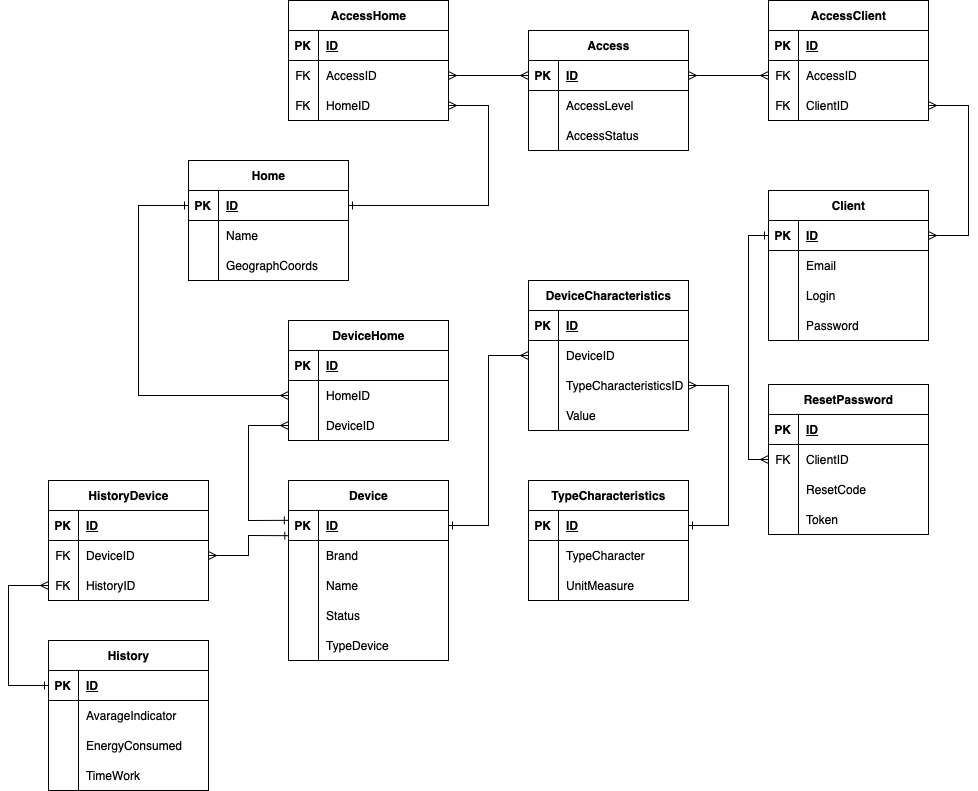
\includegraphics[width=0.9\linewidth]{img/newDB.png}
    \caption{\label{img:newDB} Диаграмма разрабатываемой базы данных}
\end{figure}
\noindent
\clearpage

На диаграмме представлены следующие таблицы:

\begin{enumerate}
    \item[1)] Client -- таблица, содержащая информацию о клиентах, 
    состоит из следующих компонентов:
    \begin{itemize}
        \item ID -- уникальный идентификатор(serial4), первичный ключ таблицы;
        \item Email -- почта пользователя (символьный тип c переменным значением, непустая строка)
        \item Login -- логин пользователя (символьный тип c переменным значением, непустая строка)
        \item Password -- пароль пользователя (символьный тип c переменным значением, непустая строка), который 
        в базе данных хранится как хешированная строка;
    \end{itemize}
    \item[2)] Access -- таблица привилегий доступа, содержащая:
    \begin{itemize}
        \item ID -- уникальный идентификатор(serial4), первичный ключ таблицы;
        \item AccessLevel -- уровень доступа пользователя к дому;
        \item AccessStatus -- текущий доступ к системе умного дома; 
    \end{itemize}
    \item[3)] AccessClient -- таблица, которая реализует отношение 
    «один-ко-многим» между таблицами «Client» и «Access», 
    имеет два уникальных идентификатора (клиент и доступ).
    \item[4)] Home -- таблица, предоставляющая информацию о домах, содержит следующие поля:
    \begin{itemize}
        \item ID -- уникальный идентификатор(serial4), первичный ключ таблицы;
        \item Name -- имя дома;
        \item GeographCoords -- географические координаты, показывающие расположение дома;
    \end{itemize}
    \item[5)] AccessHome -- таблица, которая реализует отношение 
    «один-ко-многим» между таблицами «Home» и «Access»,
    имеет два уникальных идентификатора (дом и доступ).
    \item[6)] Device -- таблица, предоставляющая информацию об устройствах, содержит следующие поля:
    \begin{itemize}
        \item ID -- уникальный идентификатор(serial4), первичный ключ таблицы;
        \item Name -- имя устройства;
        \item Brand -- бренд устройства;
        \item Status -- текущее состояние устройства;
        \item TypeDevice -- тип устройства;
    \end{itemize}
    \item[7)] DeviceHome -- таблица, которая реализует отношение 
    «многие-ко-многим» между таблицами «Device» и «Home»,
    имеет два уникальных идентификатора (устройство и дом).
    \item[8)] History -- таблица, содержащая историю работы устройств, имеет следующие поля:
    \begin{itemize}
        \item ID -- уникальный идентификатор(serial4), первичный ключ таблицы;
        \item AvarageIndicator -- средний показатель характеристики устройства;
        \item EnergyConsumed -- потребленная энергия устройством за время работы;
        \item TimeWork -- время работы устройства;
    \end{itemize}
    \item[9)] HistoryDevice -- таблица, которая реализует отношение 
    «многие-ко-многим» между таблицами «Device» и «History»,
    имеет два уникальных идентификатора (устройство и история).
    \item[10)] ResetPassword -- таблица, которая необходима для восстановления пароля пользов ателя, она содержит:
    \begin{itemize}
        \item ID -- уникальный идентификатор(serial4), первичный ключ таблицы;
        \item ClientID -- уникальный идентификатор пользователя, который восстанавливает пароль;
        \item ResetCode -- код, необходимый для подтверждения проверки пользователя;
        \item Token - токен доступа.
    \end{itemize}
        
    
\end{enumerate}

\section{Функции базы данных}

Когда устройство начинает работать, необходимо обновлять 
статус для того, чтобы пользователь
мог увидеть текущее состояние устройства. 
Для этого была описана функция, которая после окончания работы
обновляет статус устройства с «Active» на «Inactive» и 
при запуске устройства с «Inactive» на «Active». 
Схема алгоритма данной функции указана на следующем рисунке
\ref{pic:func1}:

\begin{figure}[h]
    \centering 
    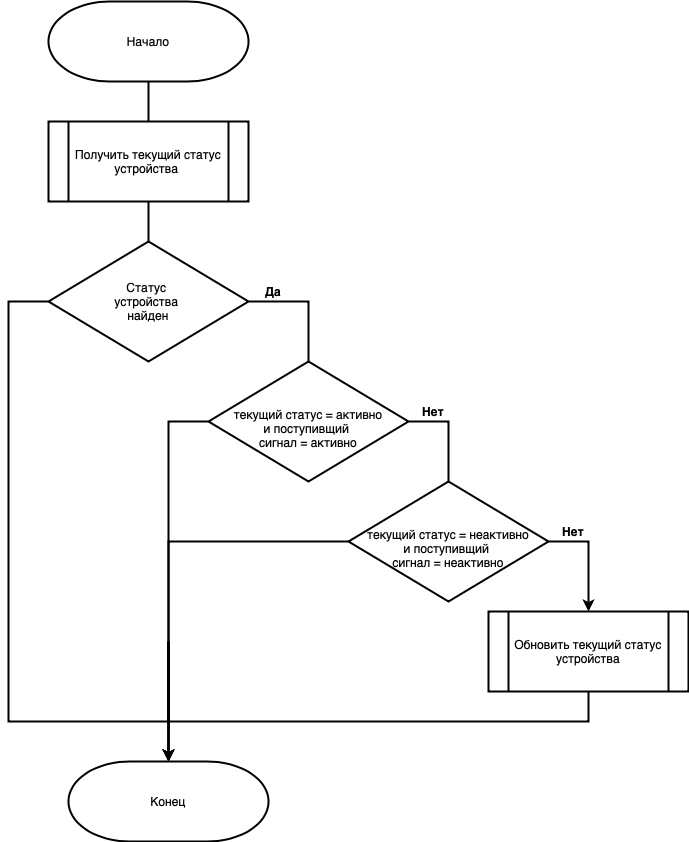
\includegraphics[width=0.6\linewidth]{img/updatestatusfunc.png}
    \caption{ER-диаграмма в нотации Чена}
    \label{pic:func1}
\end{figure}
\noindent
\clearpage

\section{Роли базы данных}

Для управления доступом к таблицам применяются роли. 
В аналитической части были установлены следующие роли: 
гость (неавторизованный пользователь), авторизованный 
пользователь, владелец дома и участник дома. 
Для каждой из этих ролей необходимо разработать 
соответствующие права доступа:
\begin{enumerate}
    \item[1)] гость(неавторизованный пользователь) должен
    иметь доступ на изменение и просмотр данных в таблице «Client»;
    \item[2)] авторизованный пользователь имеет все права
    гостя, так же ему предоставлены изменение и добавление данных
    в таблицу «Home»;
    \item[3)] участник дома должен иметь все права авторизованного 
    пользователя, так же ему доступен просмотр таблиц
    «History», «Device», «TypeCharacteristics», «Access», в зависимости
    от предоставленных прав владельцем дома участнику может быть
    доступно добавление, изменение данных в указанных таблицах;
    \item[3)] владелец должен иметь возможность 
    просматривать и изменять записи во всех существующих таблицах.
\end{enumerate}

\section*{Вывод}

В данном разделе были описаны сущности и построена диаграмма
базы данных, описана ипользуемая функция и приведена схема ее алгоримта.
Так же были формализованы роли на уровене базы
данных, чтобы обеспечить управление доступом к таблицам.

    \chapter{Технологическая часть}

В данном разделе происходит выбор средств 
реализации базы данных и приложения, 
листинги кода, а так же будет показан интерфейс программы.


\section{Выбор системы управления базой данных}

В аналитическом разделе была выбрана реляционная 
система управления, наиболее распространнеными представителями
данной системы являются: 
Microsoft SQL, PostgreSQL, Oracle, а также MySQL~\cite{diffdb}. 

Выберем следующие критерии для сравнения выбранных систем:
\begin{enumerate}
    \item[1)] возможность бесплатного использования;
    \item[2)] опыт работы с данной системой;
    \item[3)] наличие подробной документации. 
\end{enumerate}

Сравнение указанных систем управления базой данных(СУБД)
представлены в таблице \ref{tab:diff}:

\begin{table}[!ht]
    \centering
    \caption{\label{tab:diff} Сравнение СУБД по указаным критериям}
    \begin{tabular}{|l|l|l|l|l|}
    \hline
        СУБД & Microsoft SQL & PostgreSQL & Oracle & MySQL \\ \hline
        1 & - & + & - & +  \\ \hline
        2 & - & + & - & -  \\ \hline
        3 & + & + & + & +  \\ \hline
    \end{tabular}
\end{table}

По результатам сравнения для реляционной базы данных была выбрана PostgreSQL, так как это 
единственная система, которая удовлетворяет всем критериям.

\section{Выбор средств реализации}

Реализация части приложения,
которая обеспечивает доступ к базе данных, 
была выполнена с использованием языка программирования GoLang~\cite{golang}. 
Данный выбор обусловлен следующими причинами:

\begin{itemize}
    \item сборщик мусора, который позволяет автоматически
    освобождать память;
    \item статическая типизация, которая помогает 
    обнаруживать ошибки на этапе компиляции;
    \item встроенная поддержка параллельных вычислений, что
    позволяет делать разработку многопоточной.
\end{itemize}

Графический интерфейс был разработан с использованием HTML~\cite{html} и CSS~\cite{css},
так же был выбран язык JavaScript~\cite{jsLang} для 
обработки событий и динамического обновления элементов.

Причина выбора данных средств заключается в следующем:
\begin{itemize}
    \item HTML и CSS поддерживаются всеми основными веб-браузерами, 
    что гарантирует доступность содержимого на различных устройствах;
    \item опыт работы с HTML и CSS;
    \item JS имеет возможность получать доступ к структуре HTML-документа, 
    что позволяет манипулировать элементами, стилями, атрибутами и событиями.
\end{itemize}

\section{Выбор среды разрабоки}

В качестве среды разработки был выбран Visual Studio Code~\cite{vscode}. Данный выбор обусловлен
следующими причинами:
\begin{itemize}
    \item бесплатный доступ;
    \item поддержка выбранных языков;
    \item опыт работы в данной среде.
\end{itemize}

\section{Архитектура приложения}

Для разрабатываемого приложения была выбрана чистая архитектура~\cite{cleanArch}, то есть приложение будет 
состоять из трех слоев: графический интерфейс, бизнес-логика, доступ к данным.

Данное разделение имеет следующие преимущества:
\begin{itemize}
    \item приложение не зависит от используемых библиотек и фреймворков;
    \item удобство тестирования;
    \item возможность использования различных баз данных, так как
    бизнес-логика не зависит напрямую от используемой базы данных.
\end{itemize}

\section{Реализация ролевой модели}
Ранее были определены 3 роли: гость (неавторизованный пользователь), 
владелец дома, а также участник дома. 
В приложении Б\ref{lst:list2.sql} -- Б\ref{lst:list4.sql} представлено создание данных ролей.

\section{Реализация функции}

Функция, осуществляющая обновление текущего статуса 
устройства в зависимости от его состояния представлена 
в приложении~А\ref{lst:list1.sql}. Следует отметить, что если 
устройство работает и какой-то другой участник дома 
захочет его запустить, то фукнция вернет ошибку.  

\section{Тестирование}

Чтобы обеспечить автоматизацию тестирования
использовался пакет testcontainers~\cite{testcontainers}, который
автоматически поднимает контейнеры. Для создания таблиц 
и ограничений к ним в тестируемой базе данных, а так же
для заполнения созданных таблиц использовался пакет goose~\cite{goose}, 
необходимый для использования миграций.

Во время проведения тестов в базе данных содержалась 
следующая информация:

\begin{enumerate}
    \item устройство dev1 с статусом <<Inactive>>;
    \item устройство dev2 с статусом <<Inactive>>.
\end{enumerate}

В таблице \ref{tab:tests} приведены тесты, 
которые использовались для проверки правильности 
работы функции для изменения текущего статуса устройства.

\begin{table}[H]
    \centering
    \caption{\label{tab:tests} Тесты, используемые для проверки правильности 
    работы функции для изменения текущего статуса устройства.}
    \begin{tabular}{|l|l|l|l|l|l|}
    \hline
        Текущее & Новое  & ID & Переданный ID & Ожидаемый & Ответ \\
        состояние & состояние & устройства &  & ответ &  \\ \hline
        inactive & inactive & 1 & 1 & -3 & -3 \\ \hline
        inactive & inactive & 2 & 2 & -3 & -3 \\ \hline
        inactive & active & 2 & 2 & 0 & 0 \\ \hline
        inactive & active & 1 & 1 & 0 & 0 \\ \hline
        active & active & 2 & 2 & -2 & -2 \\ \hline
        active & inactive & 1 & 1 & 0 & 0 \\ \hline
        active & inactive & 2 & 2 & 0 & 0 \\ \hline
    \end{tabular}
\end{table}

Также были проведены тесты для других запросов к базе данных, результат которых представлен 
в приложении В\ref{img:test1} -- В\ref{img:test2}.

\section{Графический интерфейс}

Независимо от роли пользователь попадает на страницу c авторизацией \ref{img:auth}, где ему предоставляется возможность 
войти в личный аккаунт с помощью пароля и почты или зарегистрироваться в системе, также пользователь может восстановить пароль.

\begin{figure}[H]
    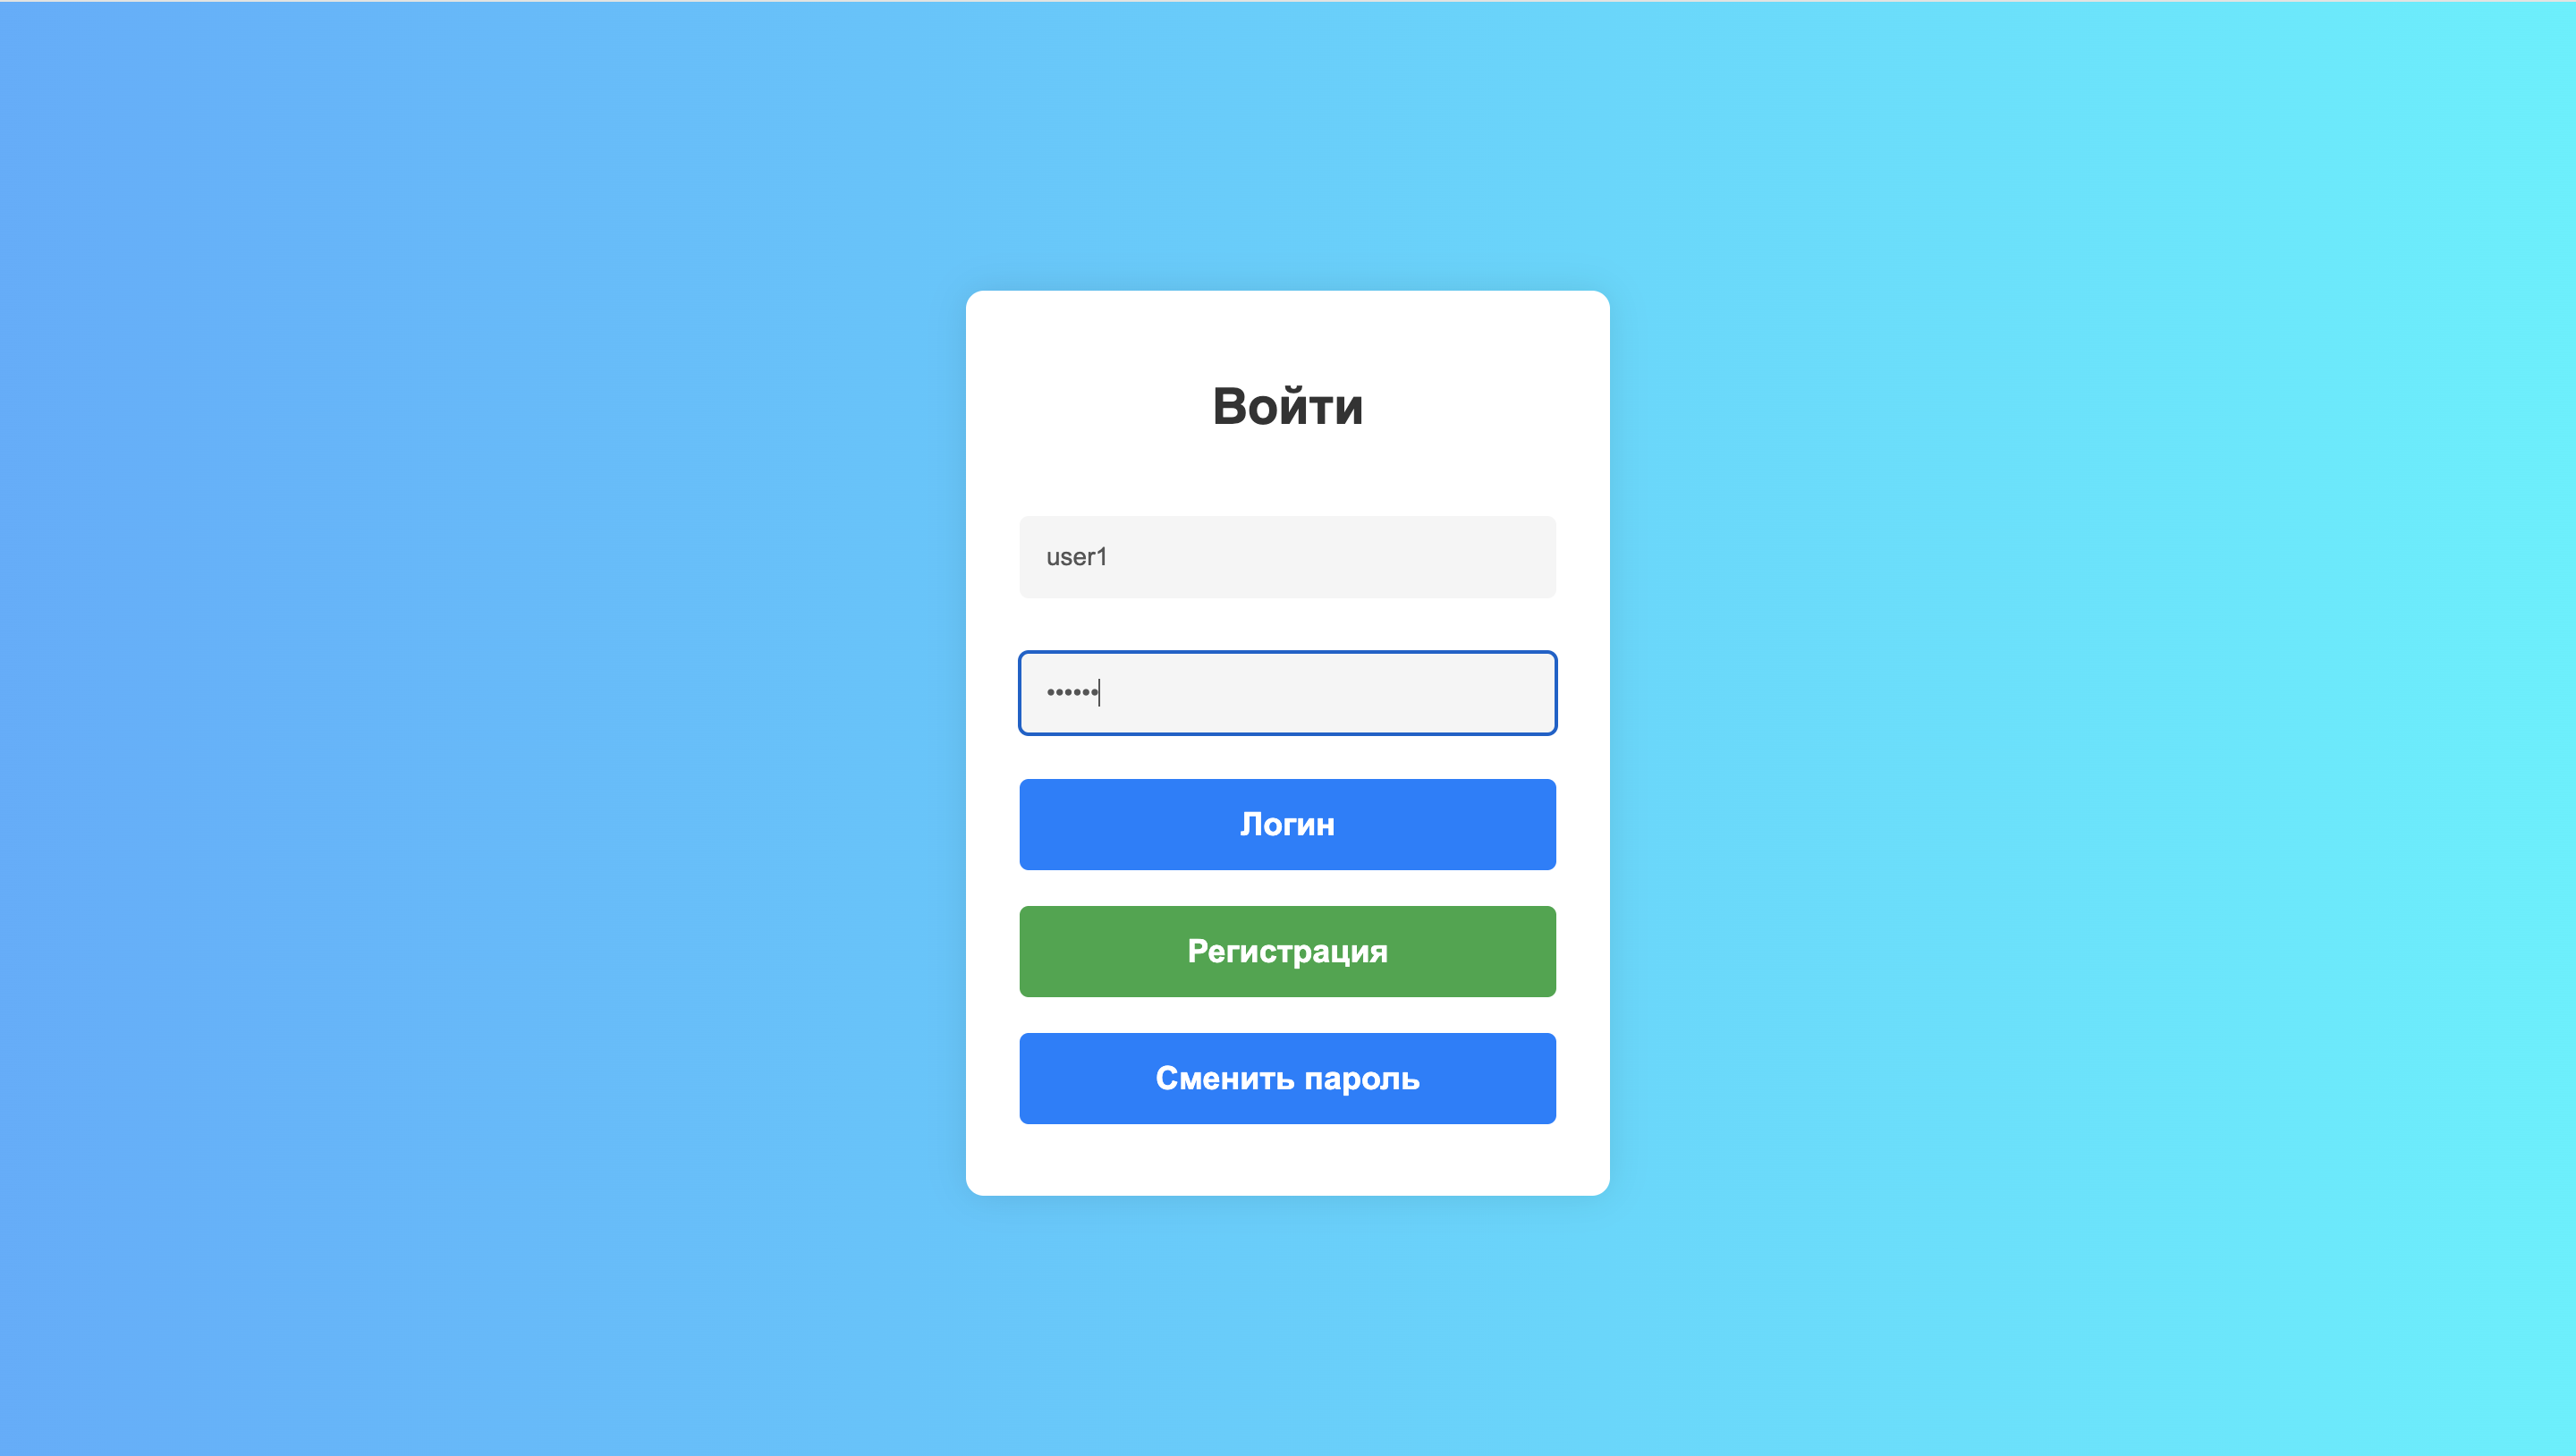
\includegraphics[width=1\linewidth]{img/auth.png}
    \caption{\label{img:auth} Страница для авторизации пользователя}
\end{figure}
\noindent

На странице регистрации пользователь может содать аккаунт, введя логин, пароль и почту \ref{img:reg}.
\begin{figure}[H]
    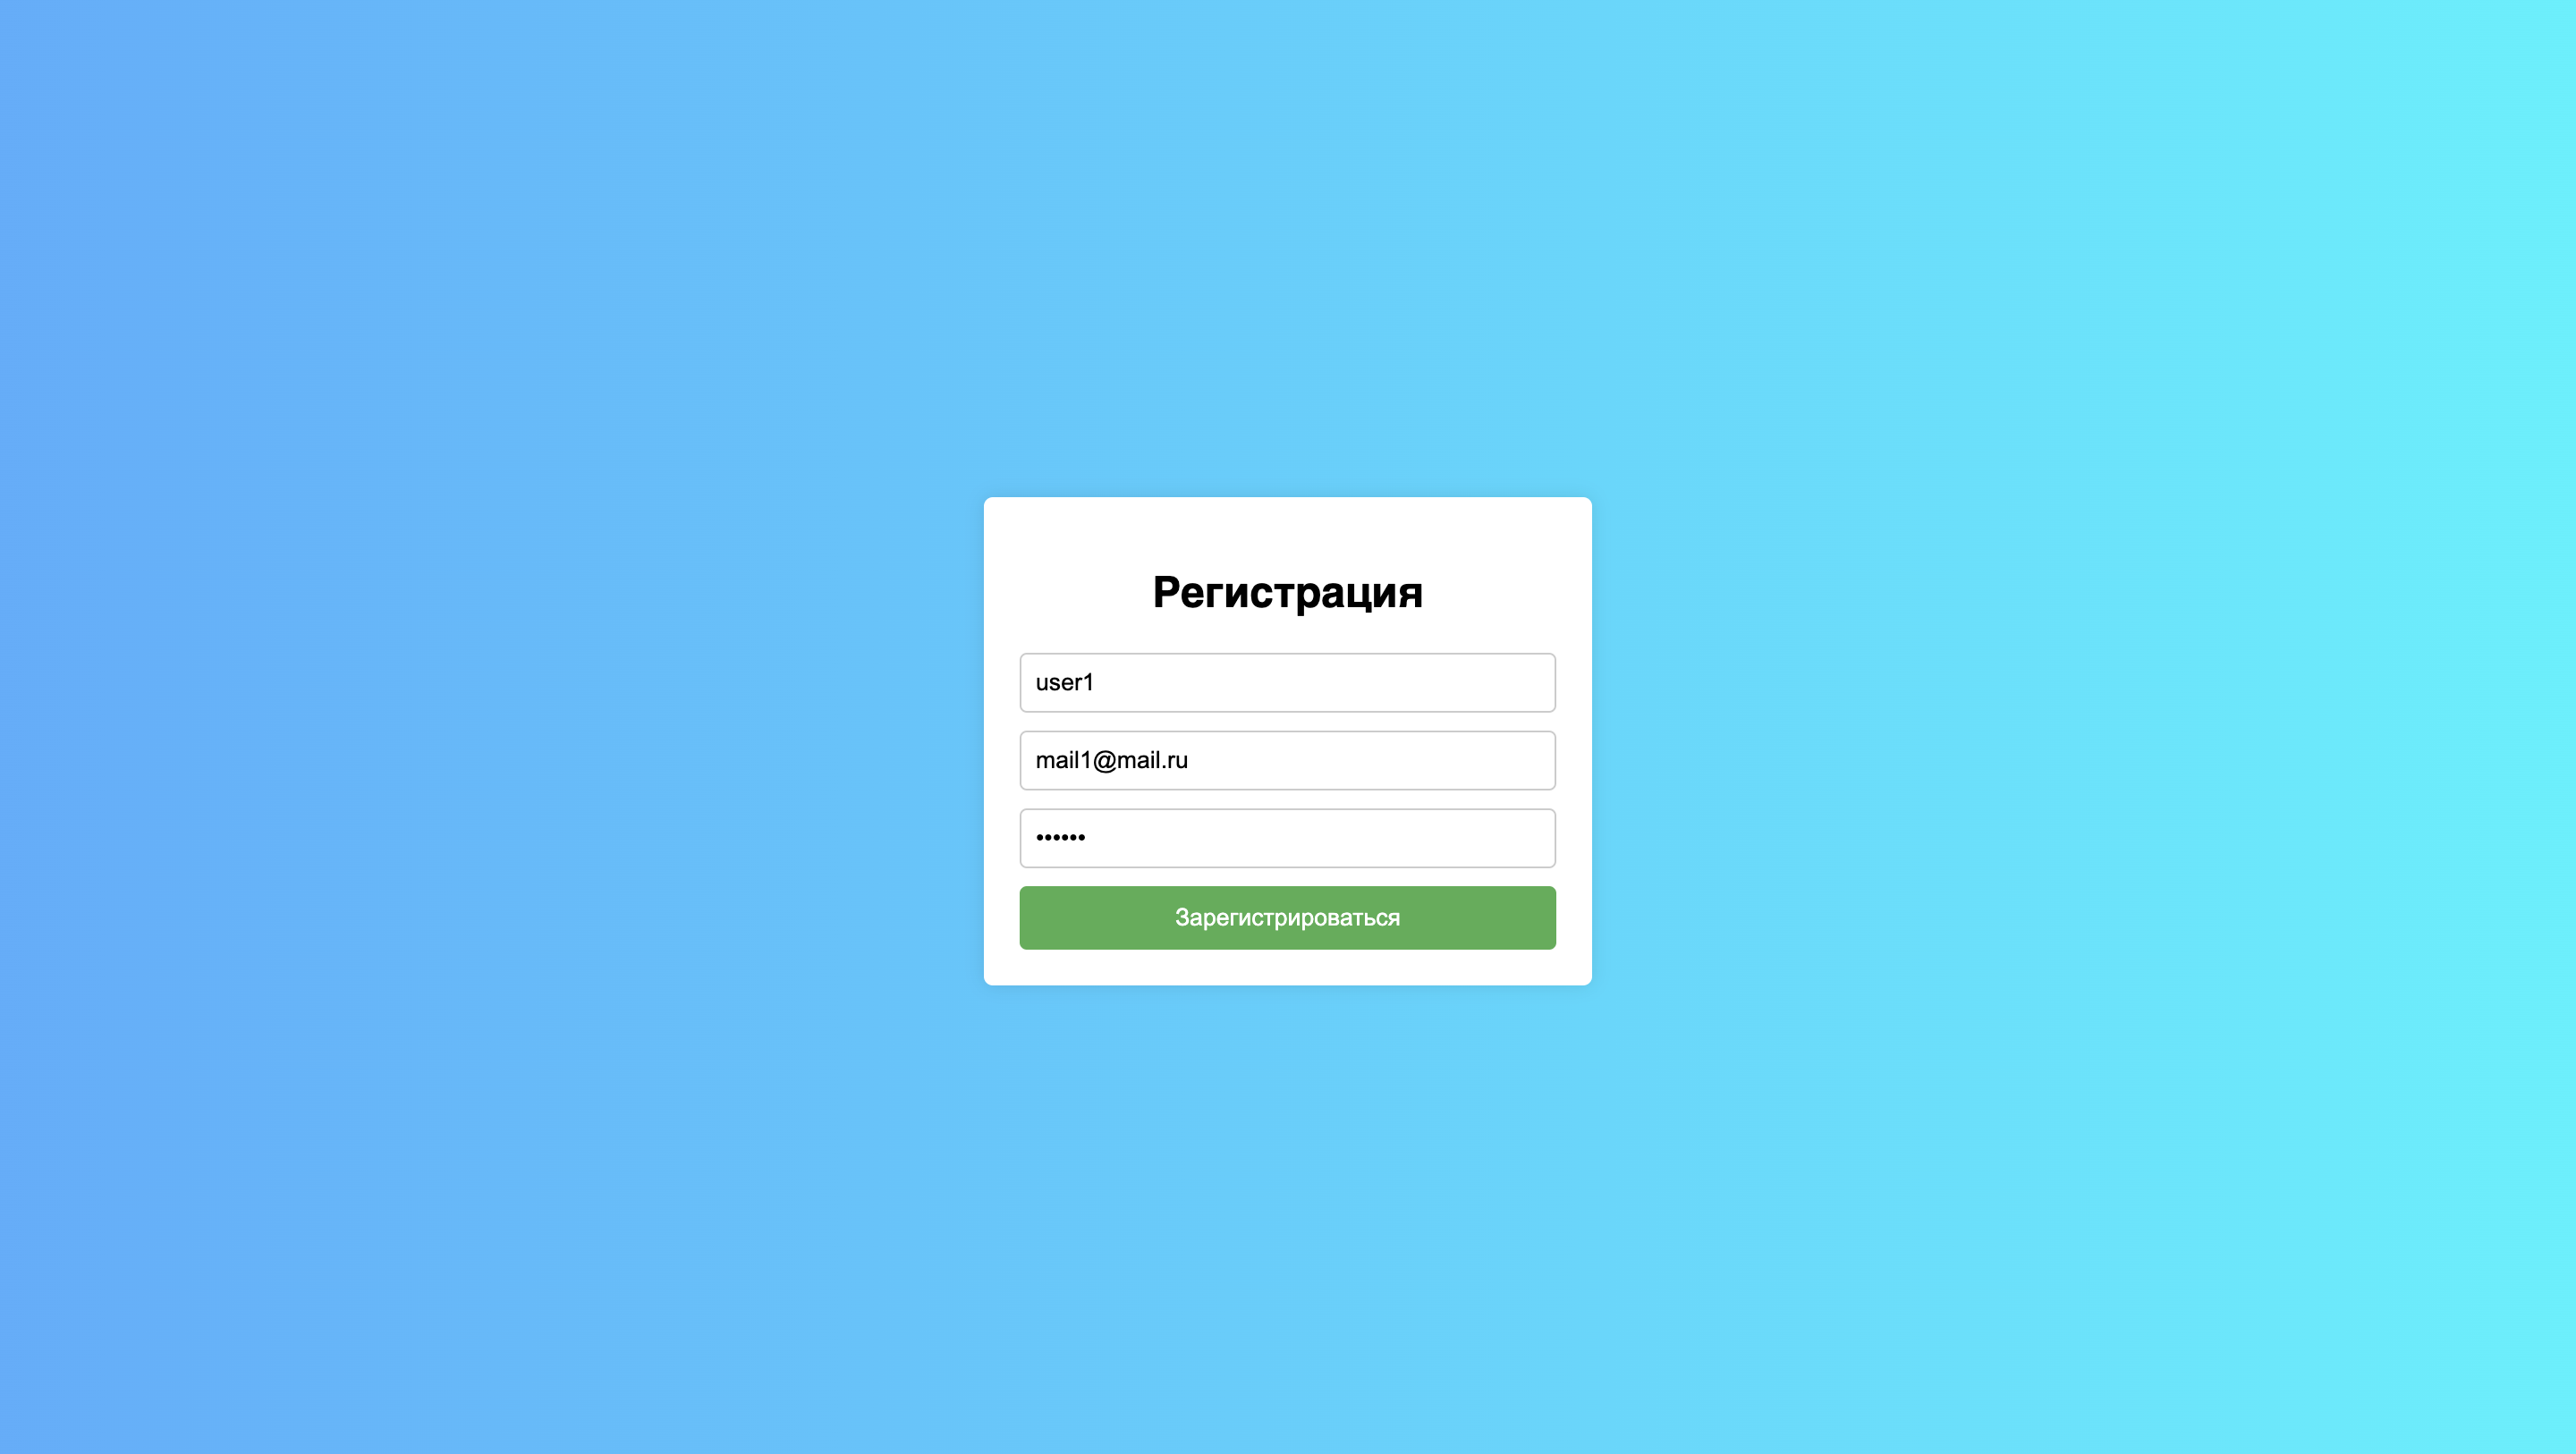
\includegraphics[width=1\linewidth]{img/reg.png}
    \caption{\label{img:reg} Страница для регистрации пользователя}
\end{figure}
\noindent

На рисуне \ref{img:passw} показана страница с восстановлением пароля. Пользователю необходимо ввести почту, которую он использовал при 
регистрации. 

\begin{figure}[H]
    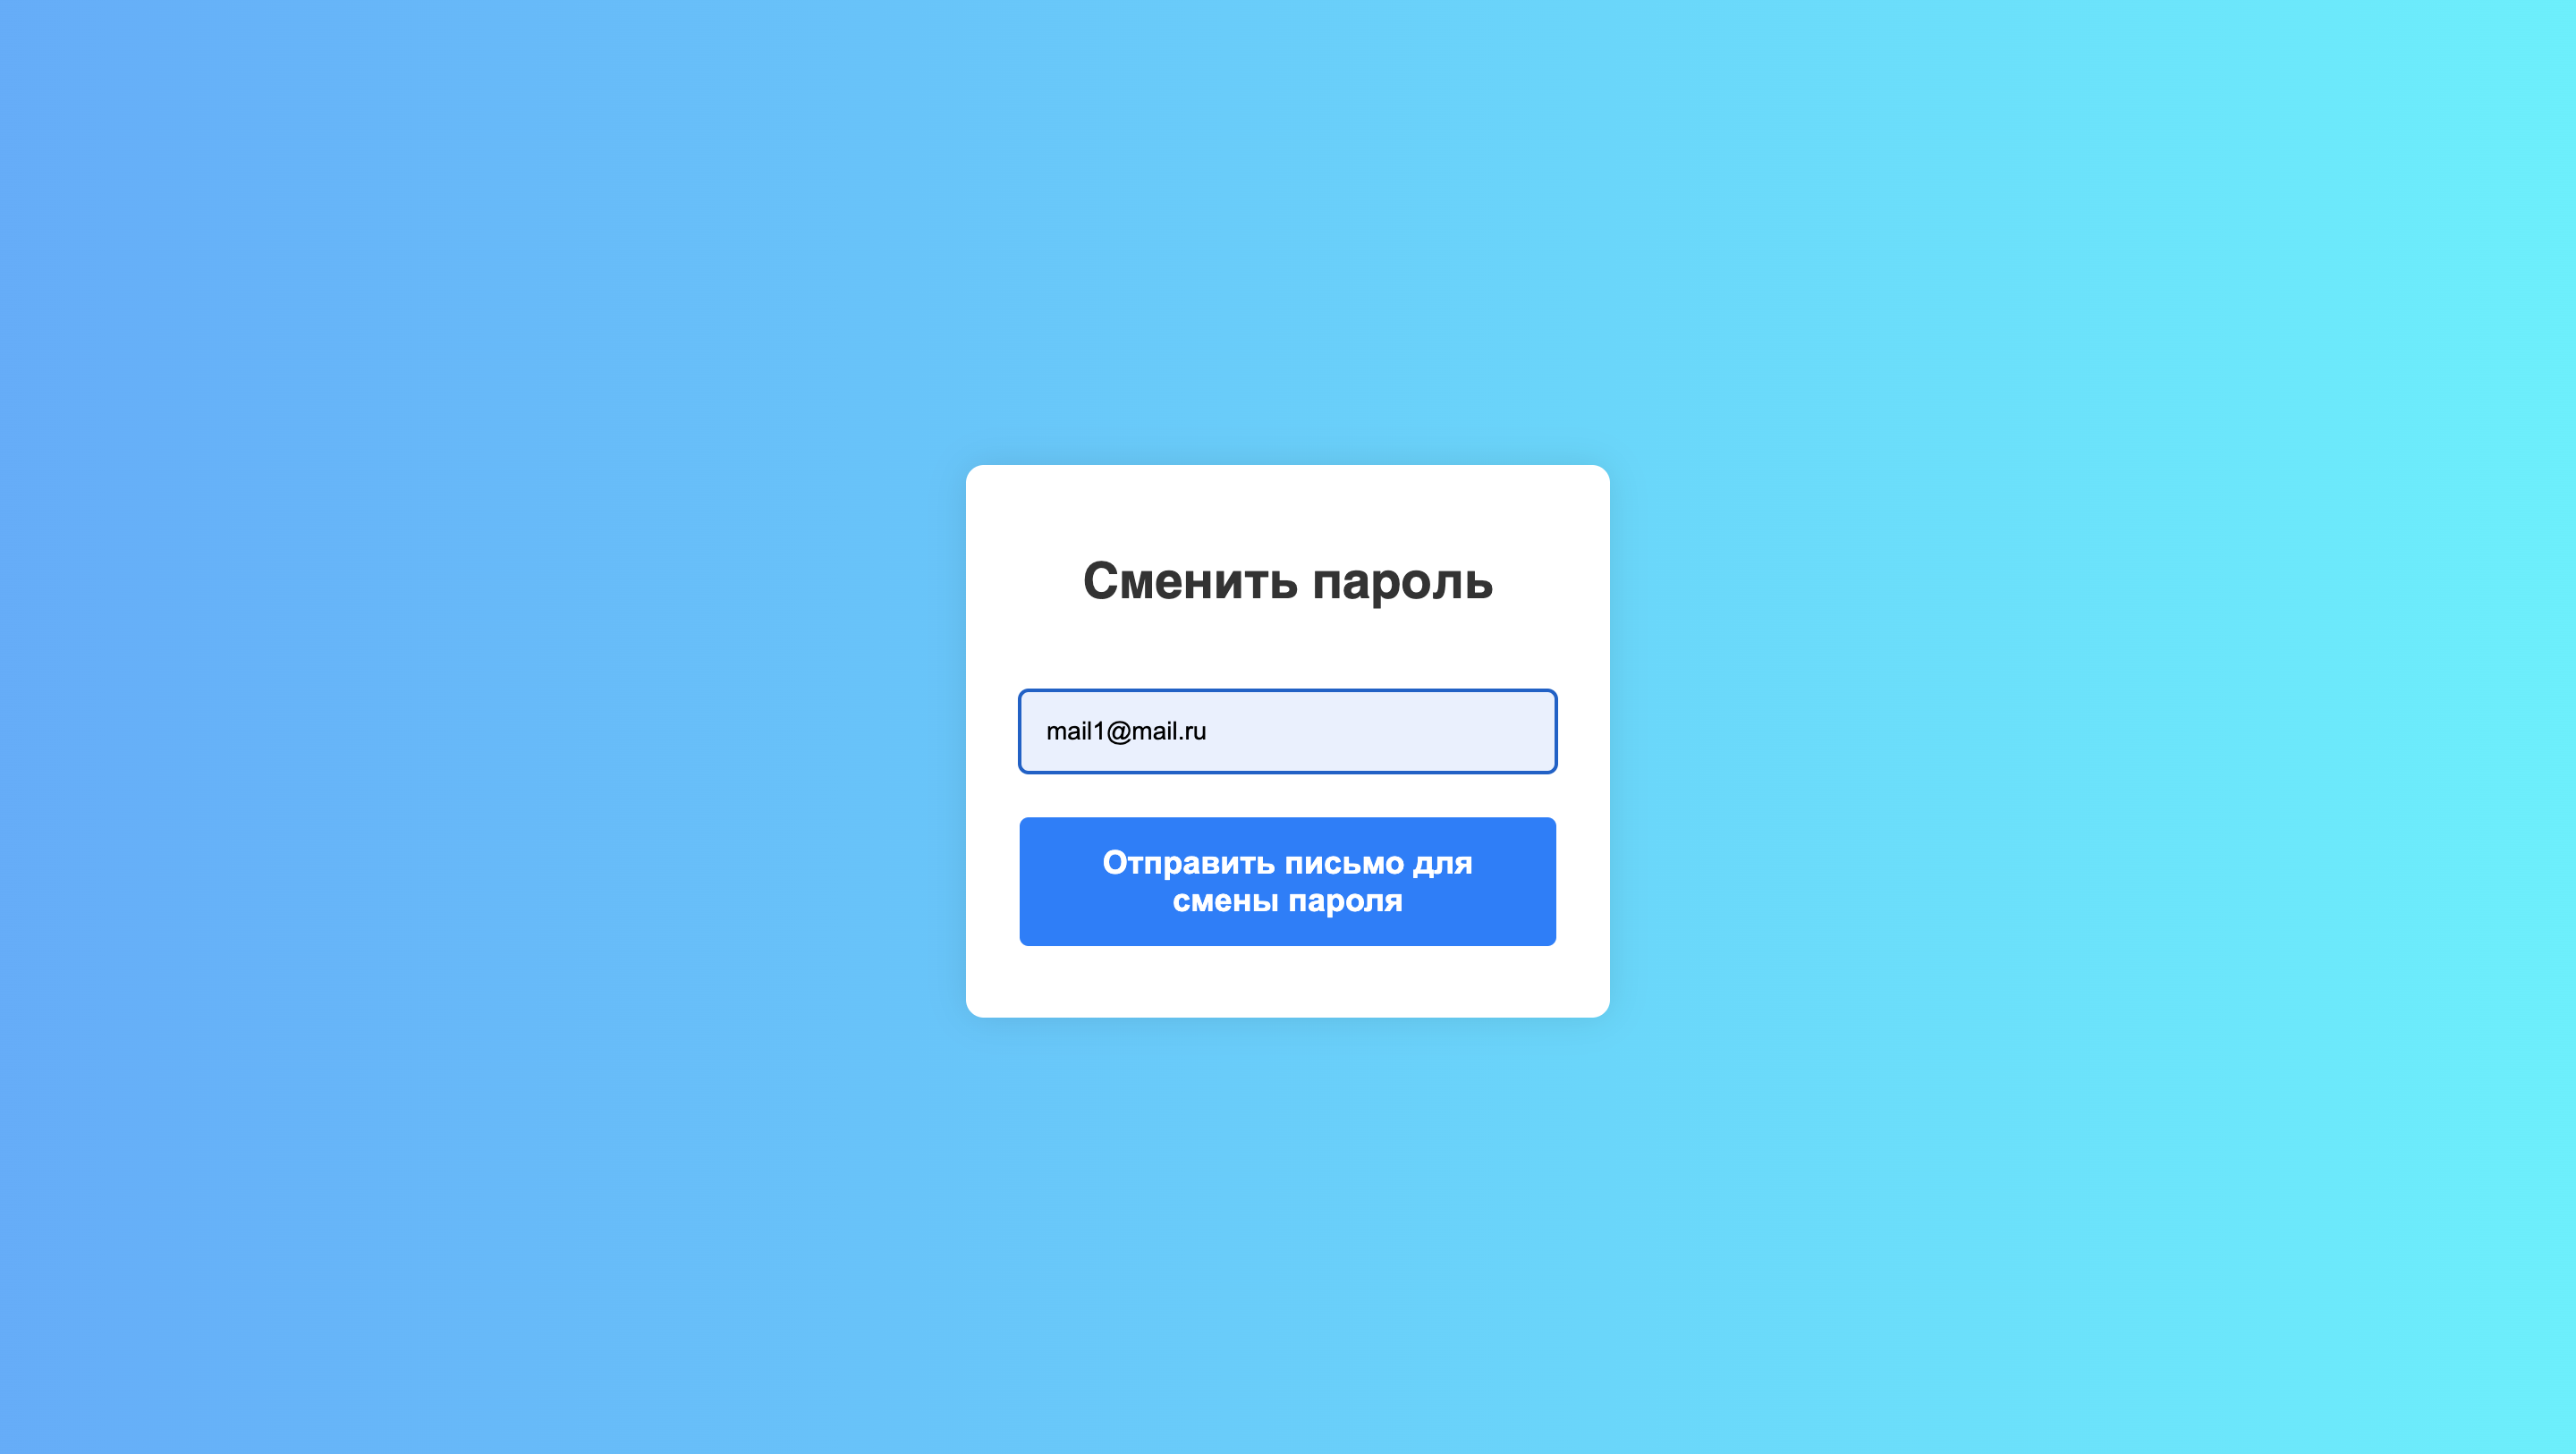
\includegraphics[width=1\linewidth]{img/passw.png}
    \caption{\label{img:passw} Страница с вводом почты для смены пароля}
\end{figure}
\noindent

На указанную почту будет выслан код, который необходимо ввести на странице \ref{img:code}.

\begin{figure}[H]
    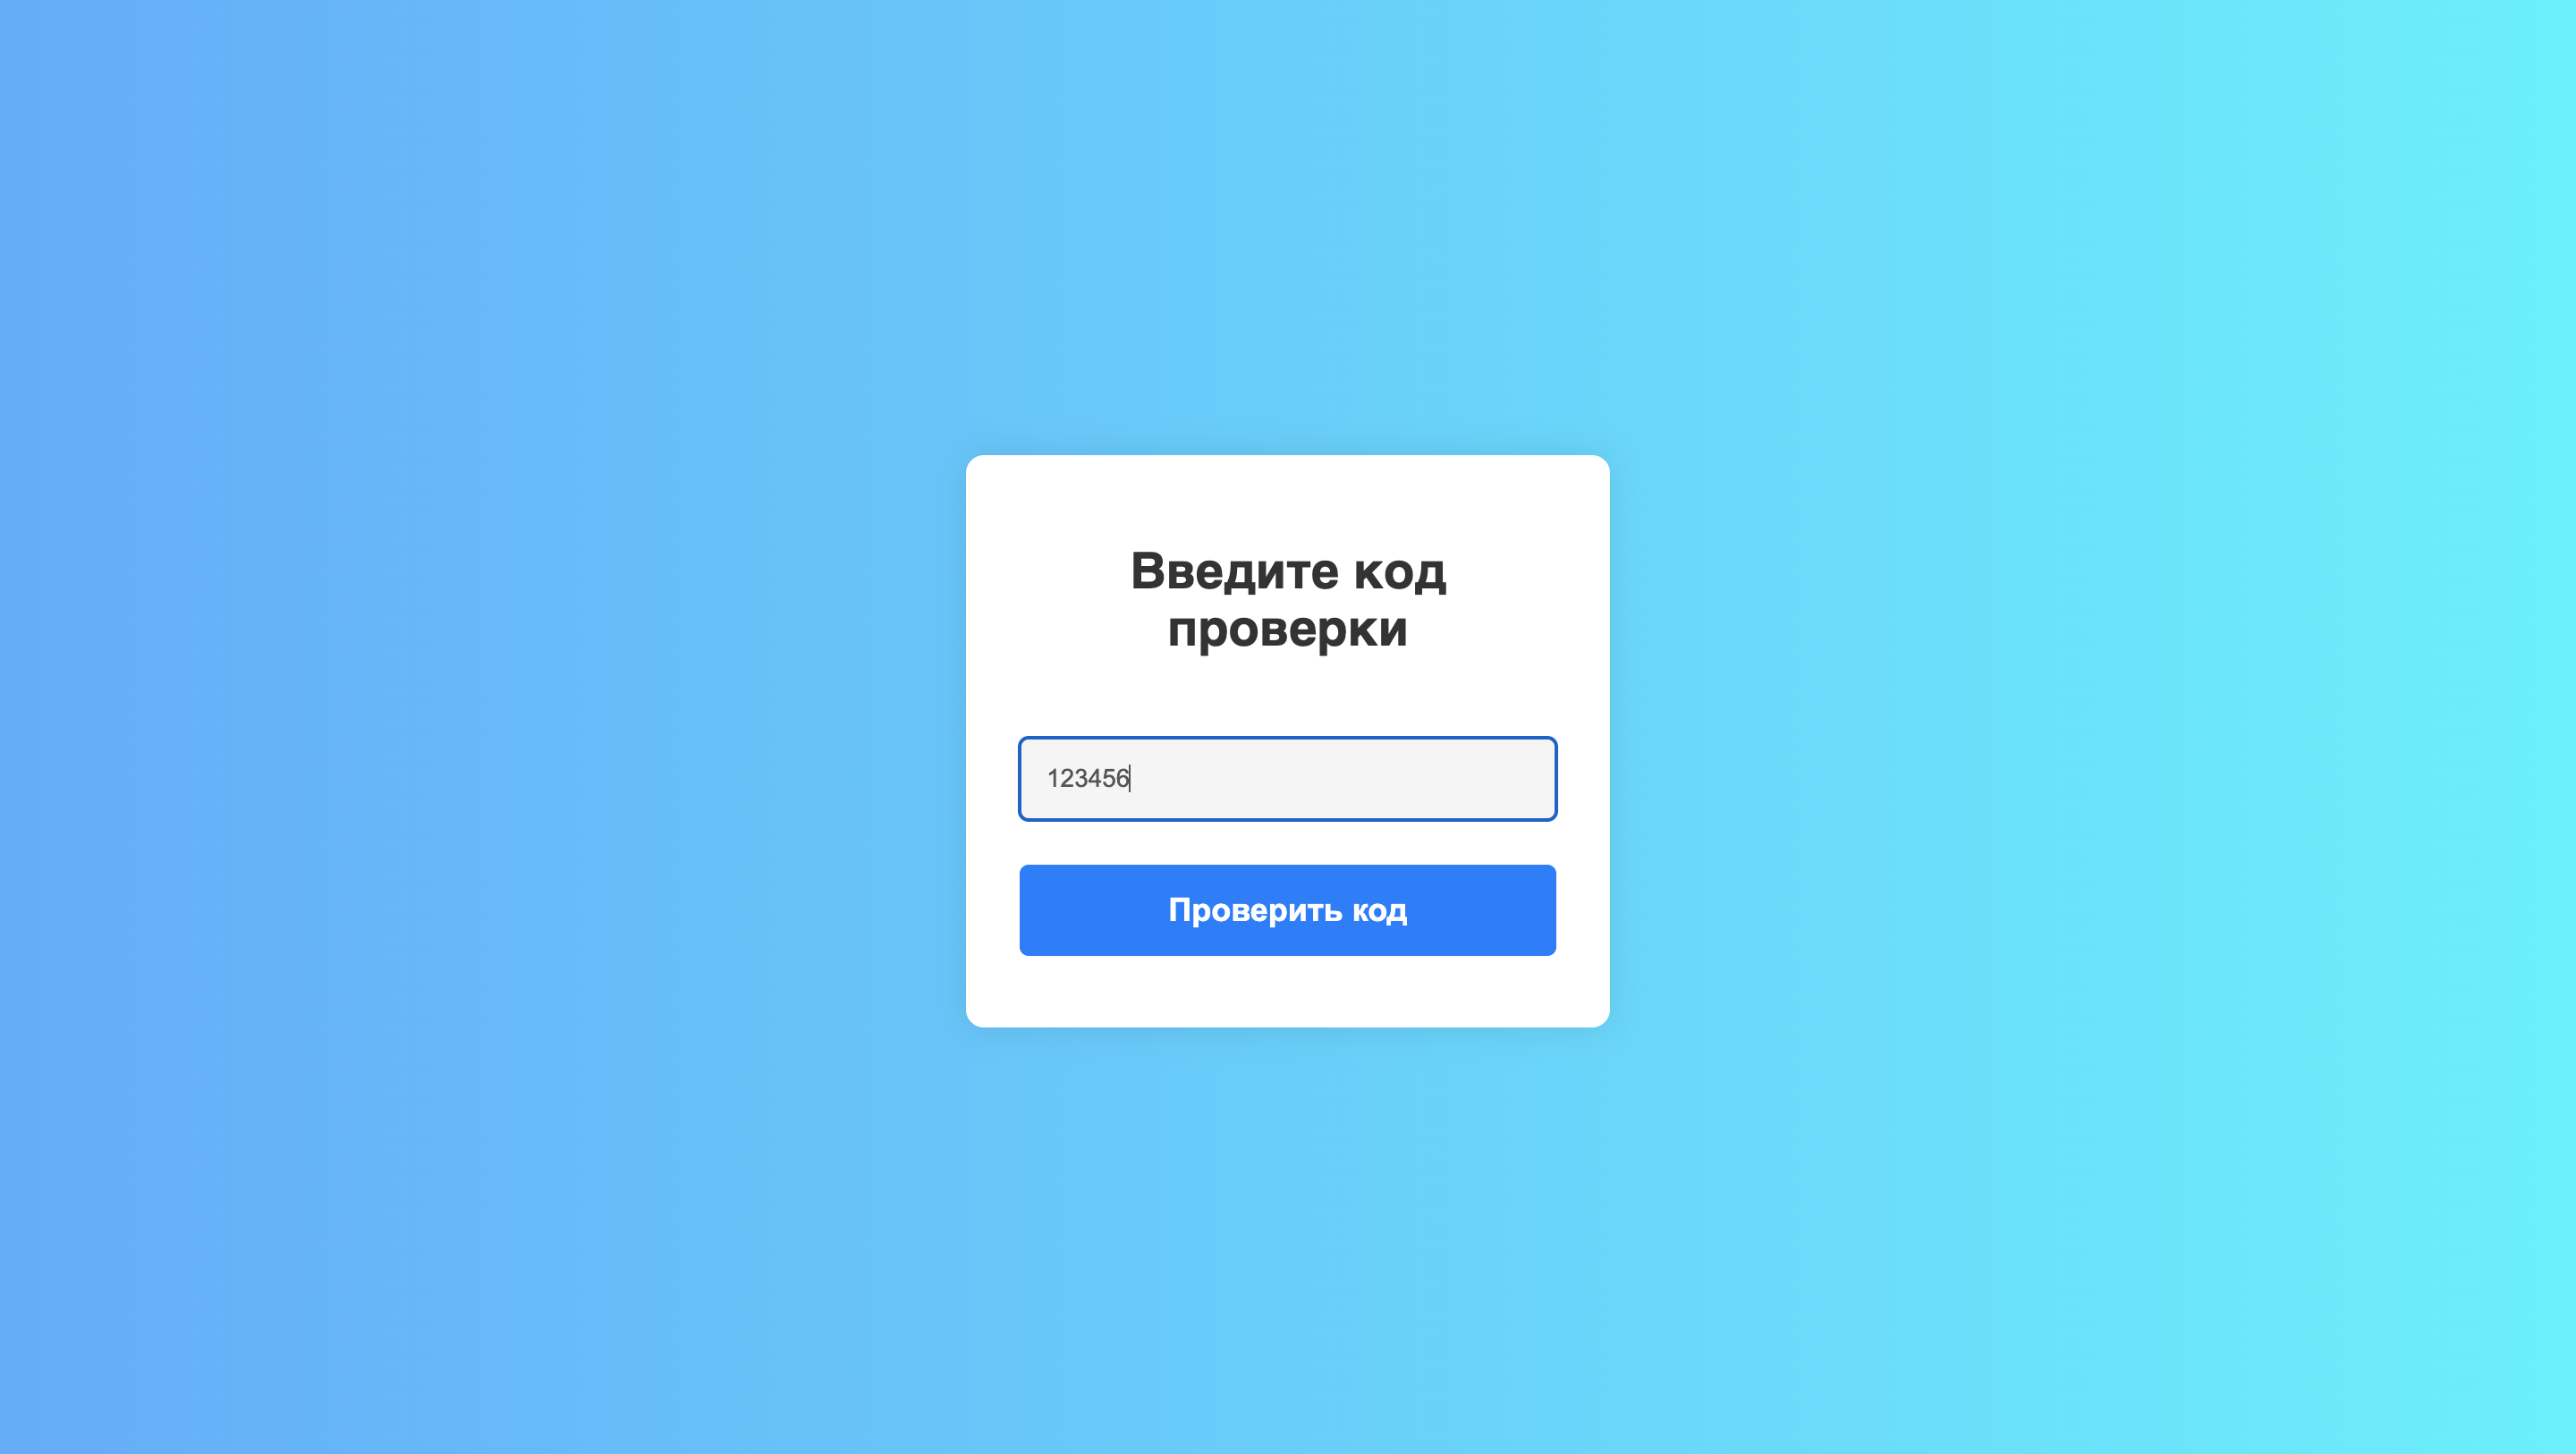
\includegraphics[width=1\linewidth]{img/code.png}
    \caption{\label{img:code} Страница с вводом кода проверки}
\end{figure}
\noindent

Далее пользователю будет предложено сменить пароль \ref{img:smena}.

\begin{figure}[H]
    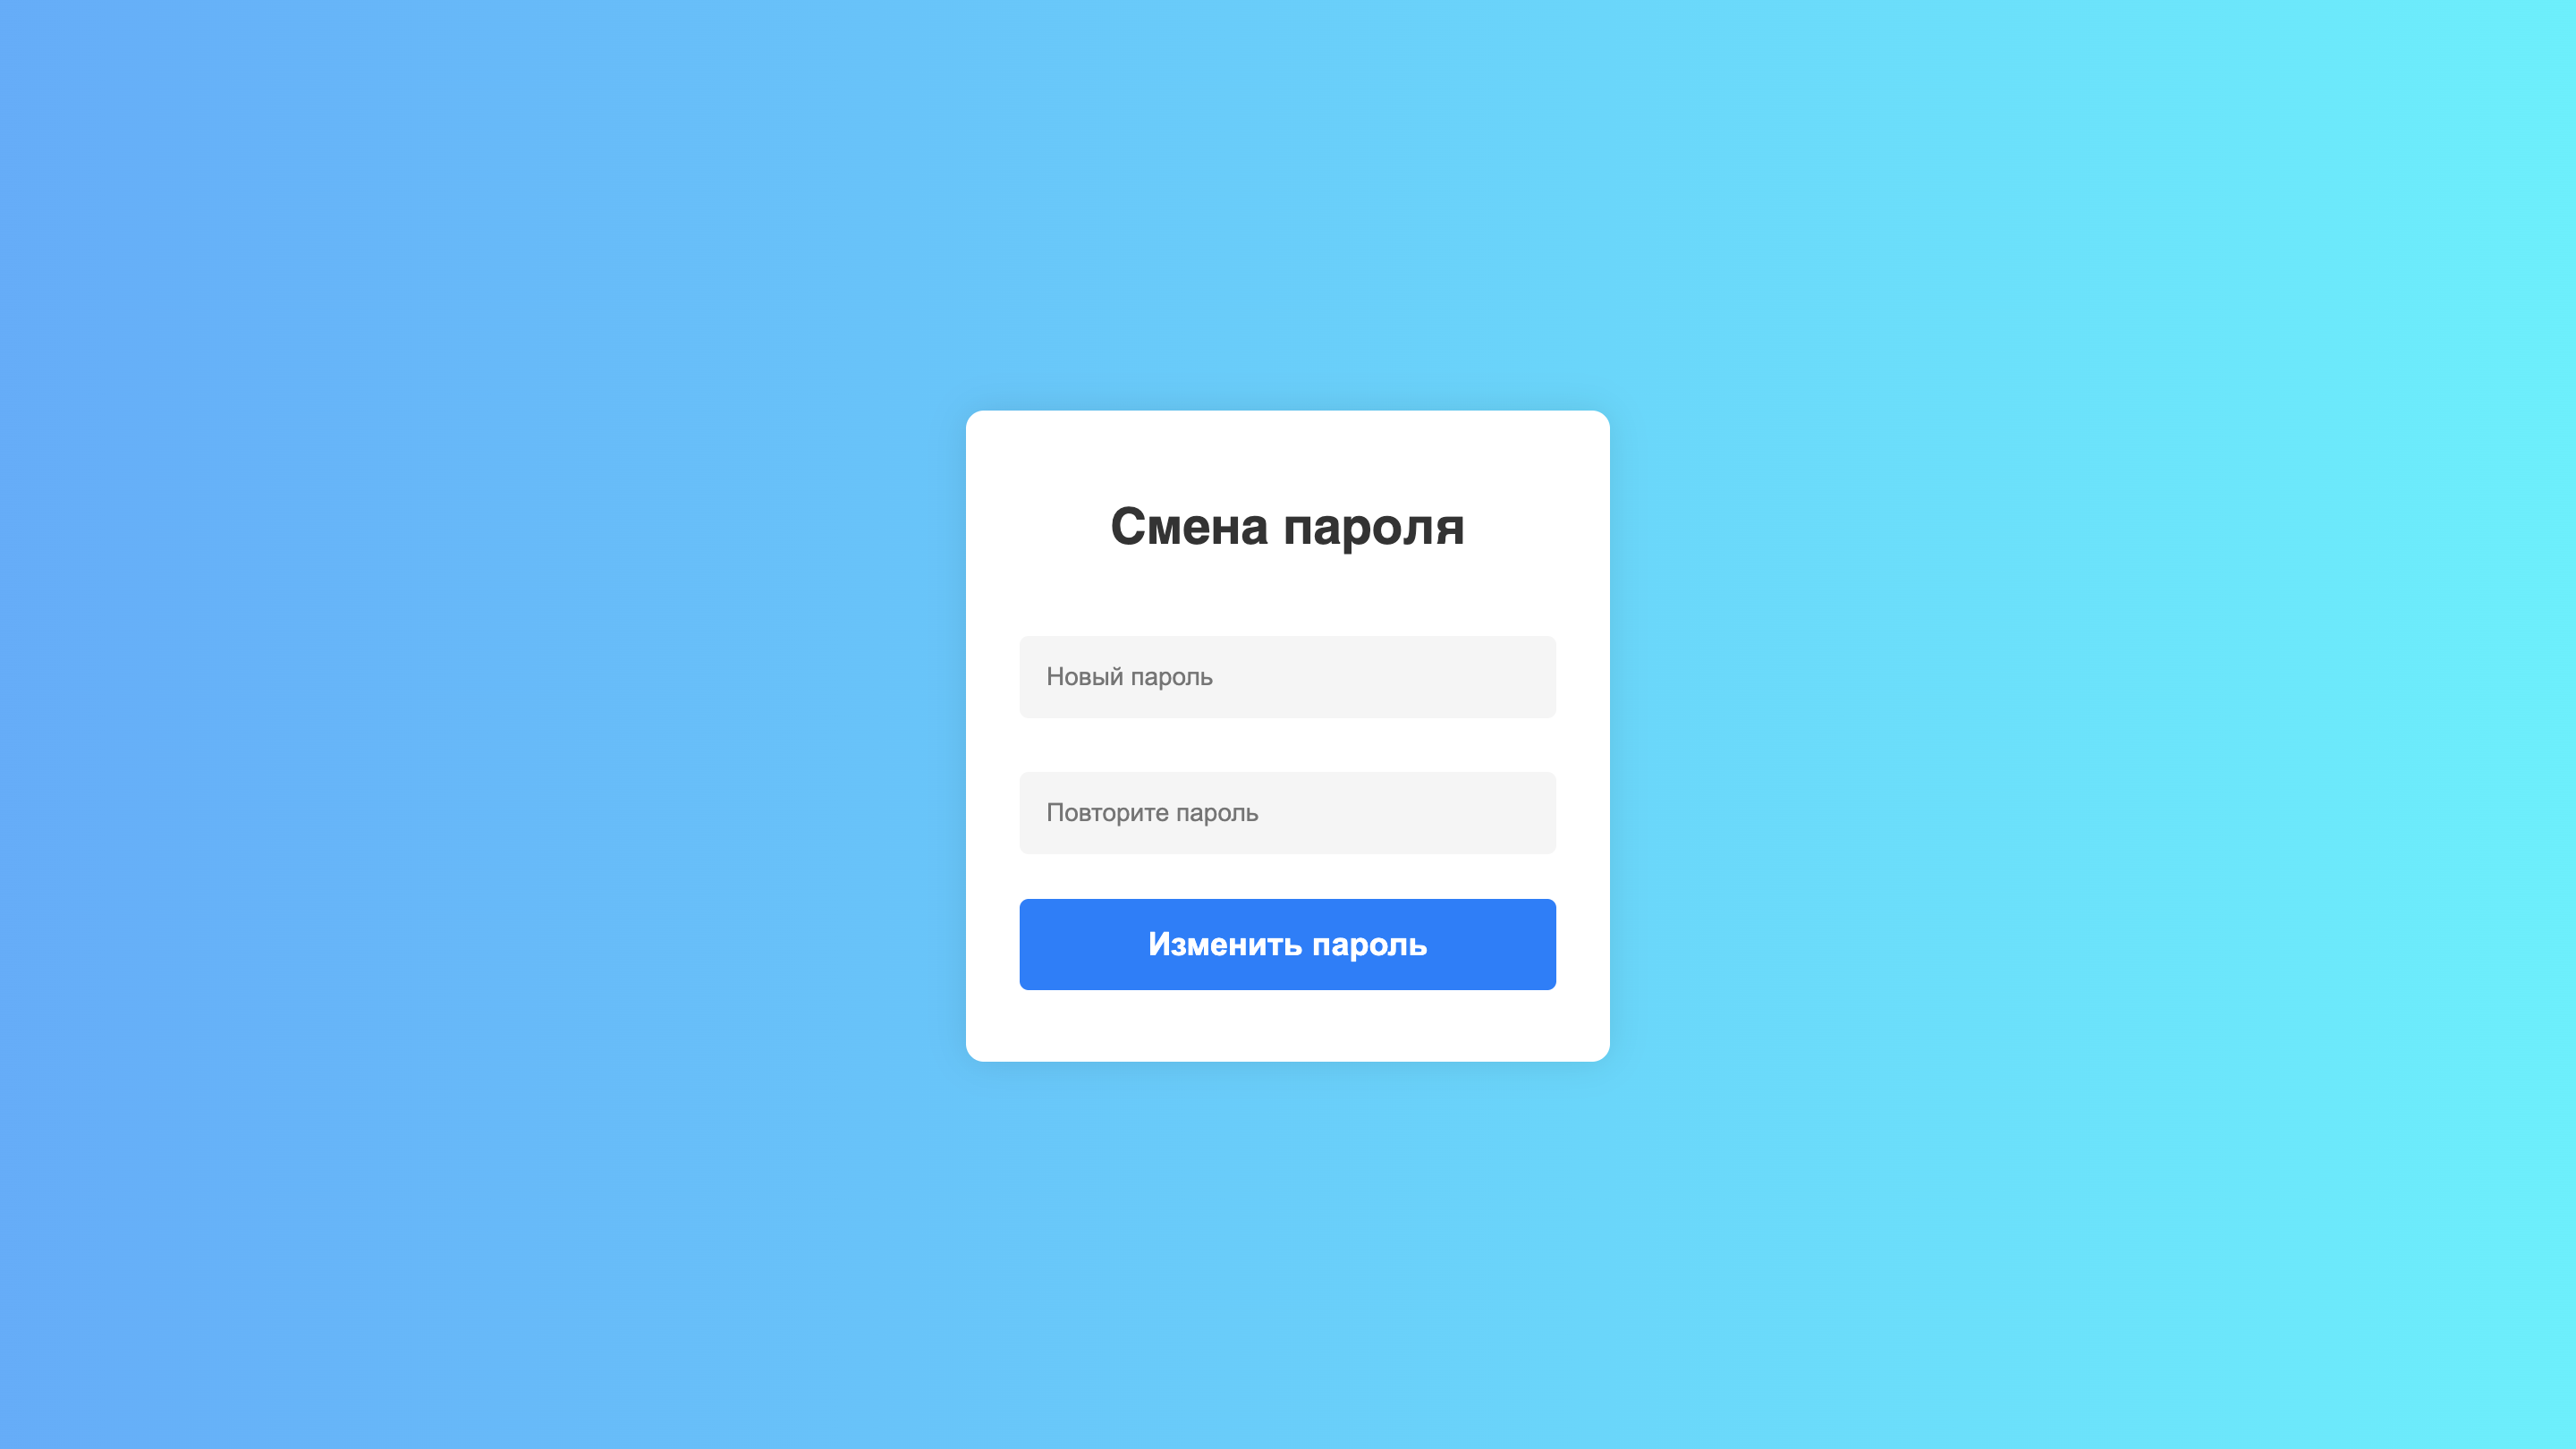
\includegraphics[width=1\linewidth]{img/smena.png}
    \caption{\label{img:smena} Страница со сменой пароля}
\end{figure}
\noindent

После авторизации пользователь будет перемещен в меню, которое содержит кнопки для перехода на 
страницы дома, устройств и прав доступа \ref{img:menu}.

\begin{figure}[H]
    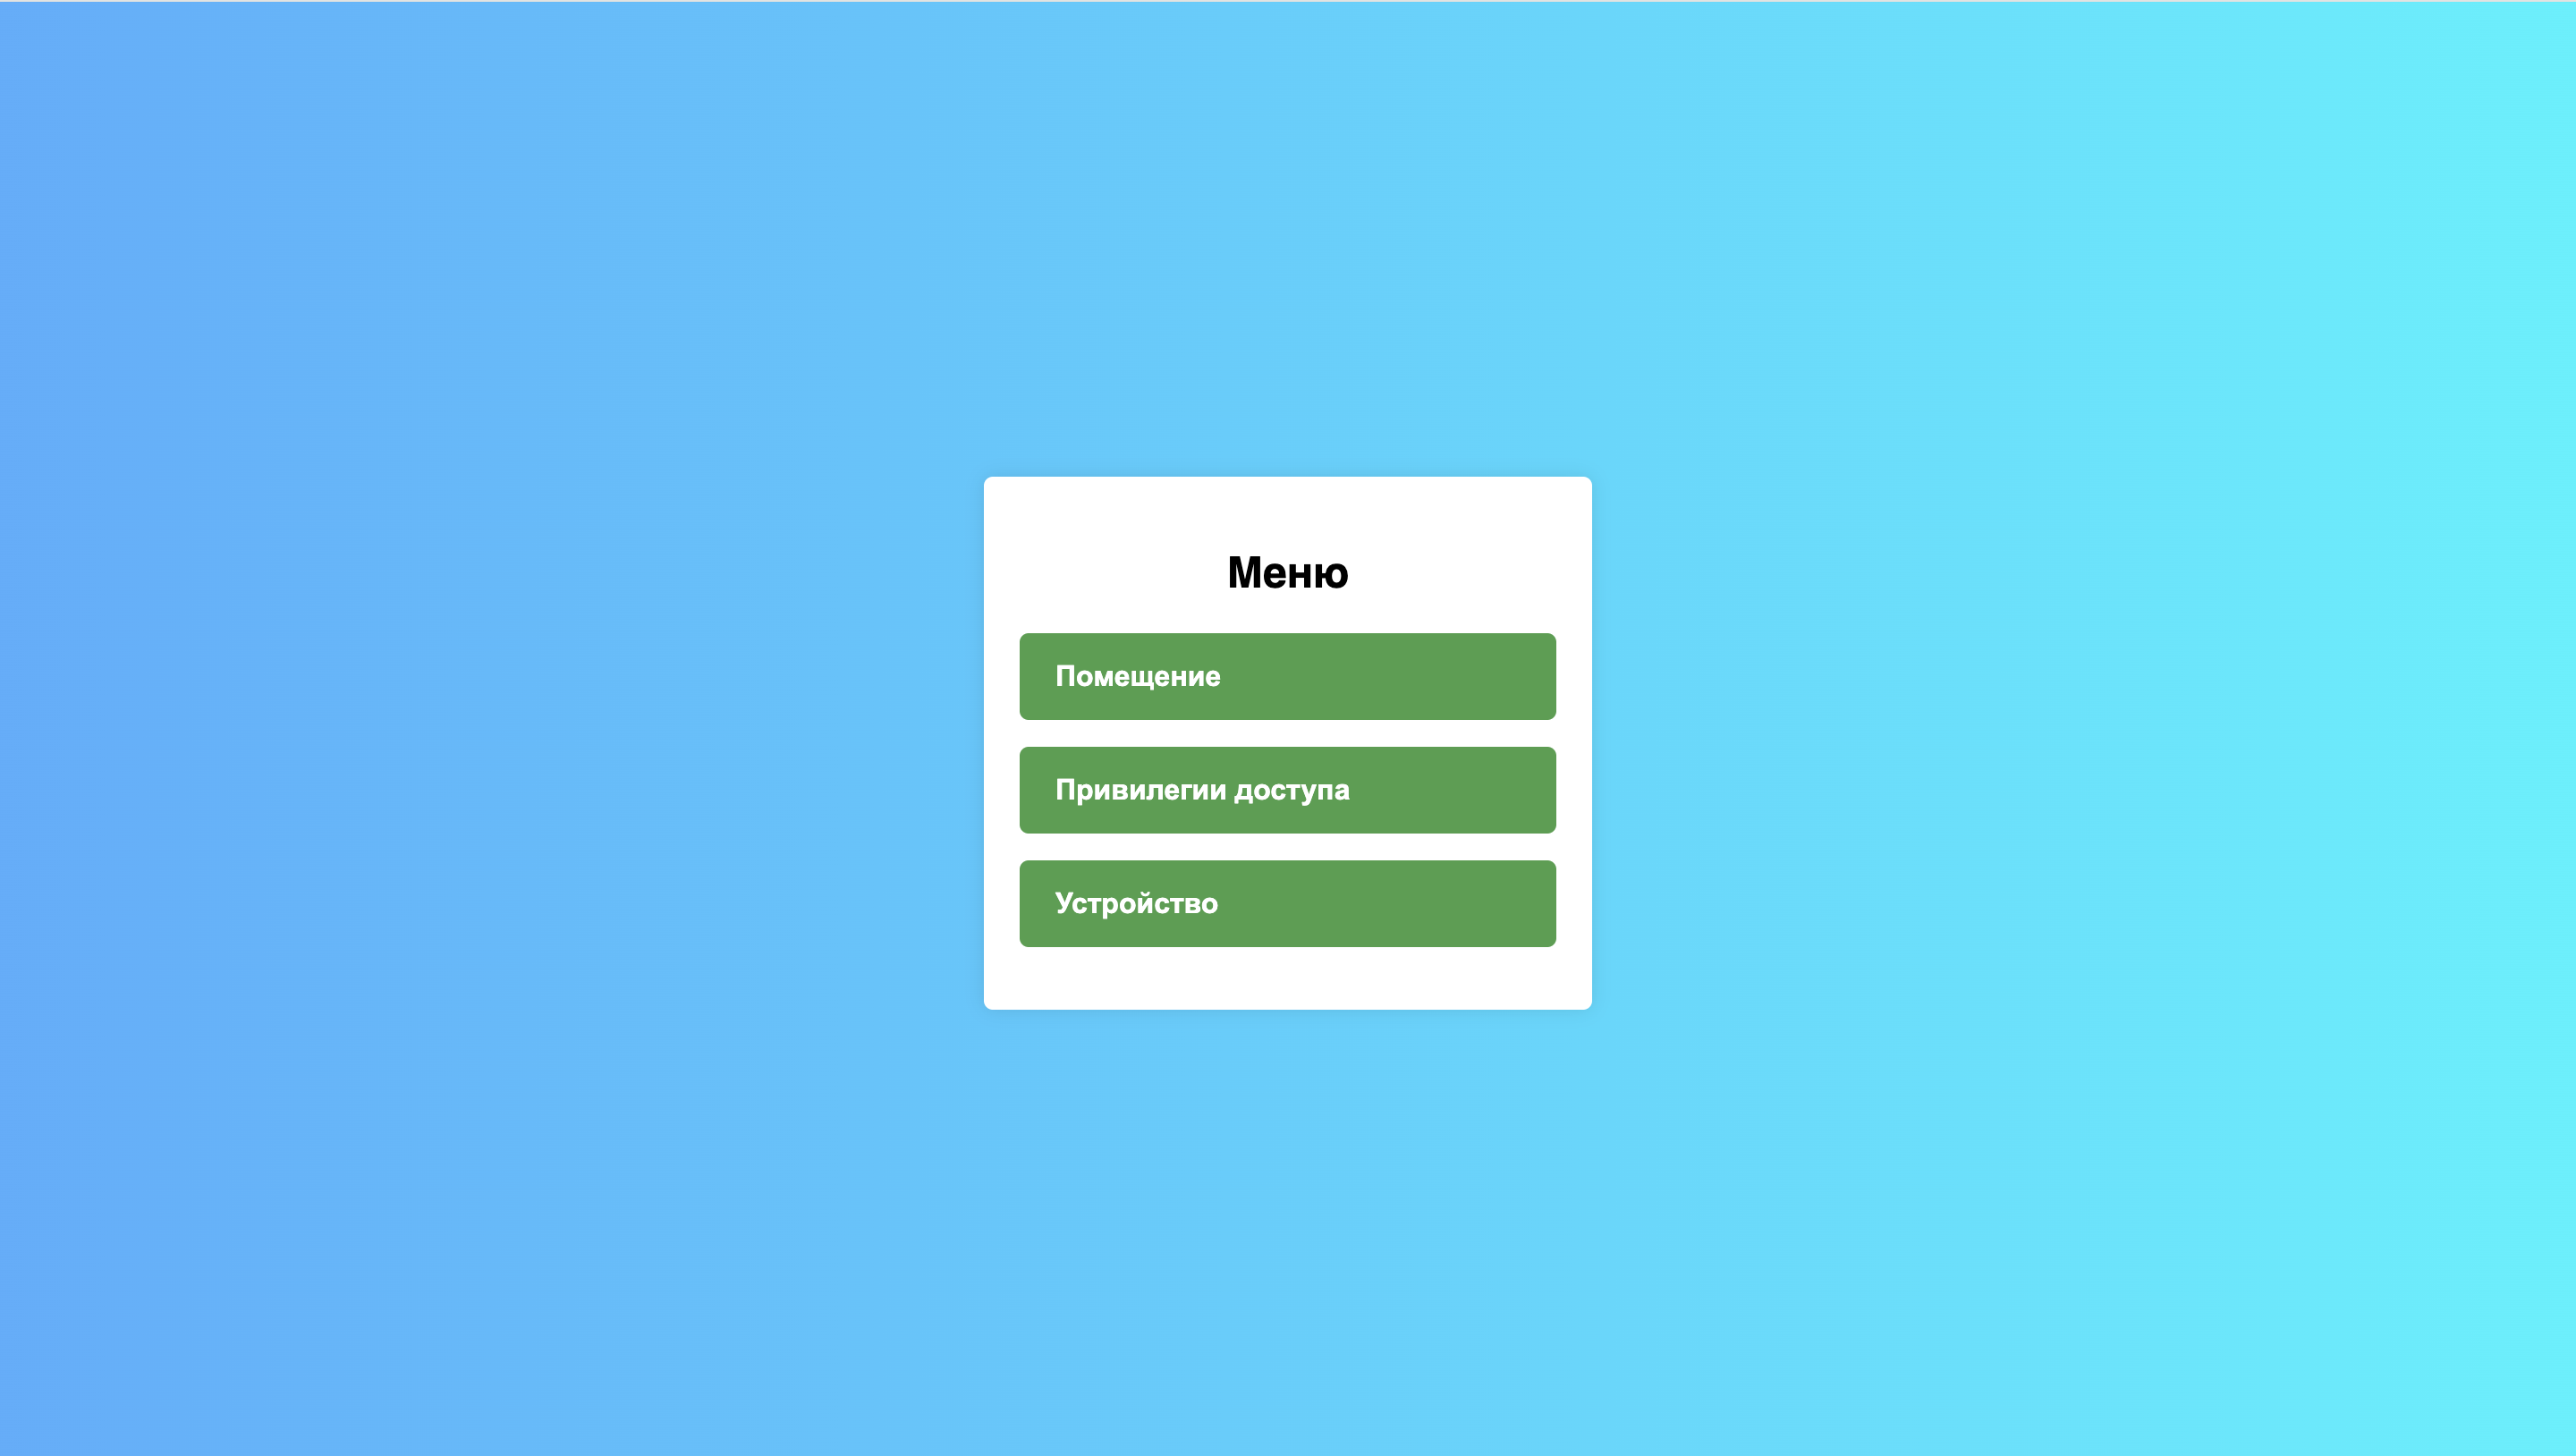
\includegraphics[width=1\linewidth]{img/menu.png}
    \caption{\label{img:menu} Страница со сменой пароля}
\end{figure}
\noindent

При нажатии на кнопу «Помещение» пользователь перейдет на страницу управления домом \ref{img:home}. На данной странице 
предоставляется возможность создать или удалить дом, обновить его имя, а также просмотреть список домов, которыми владеет 
пользователь. 

\begin{figure}[H]
    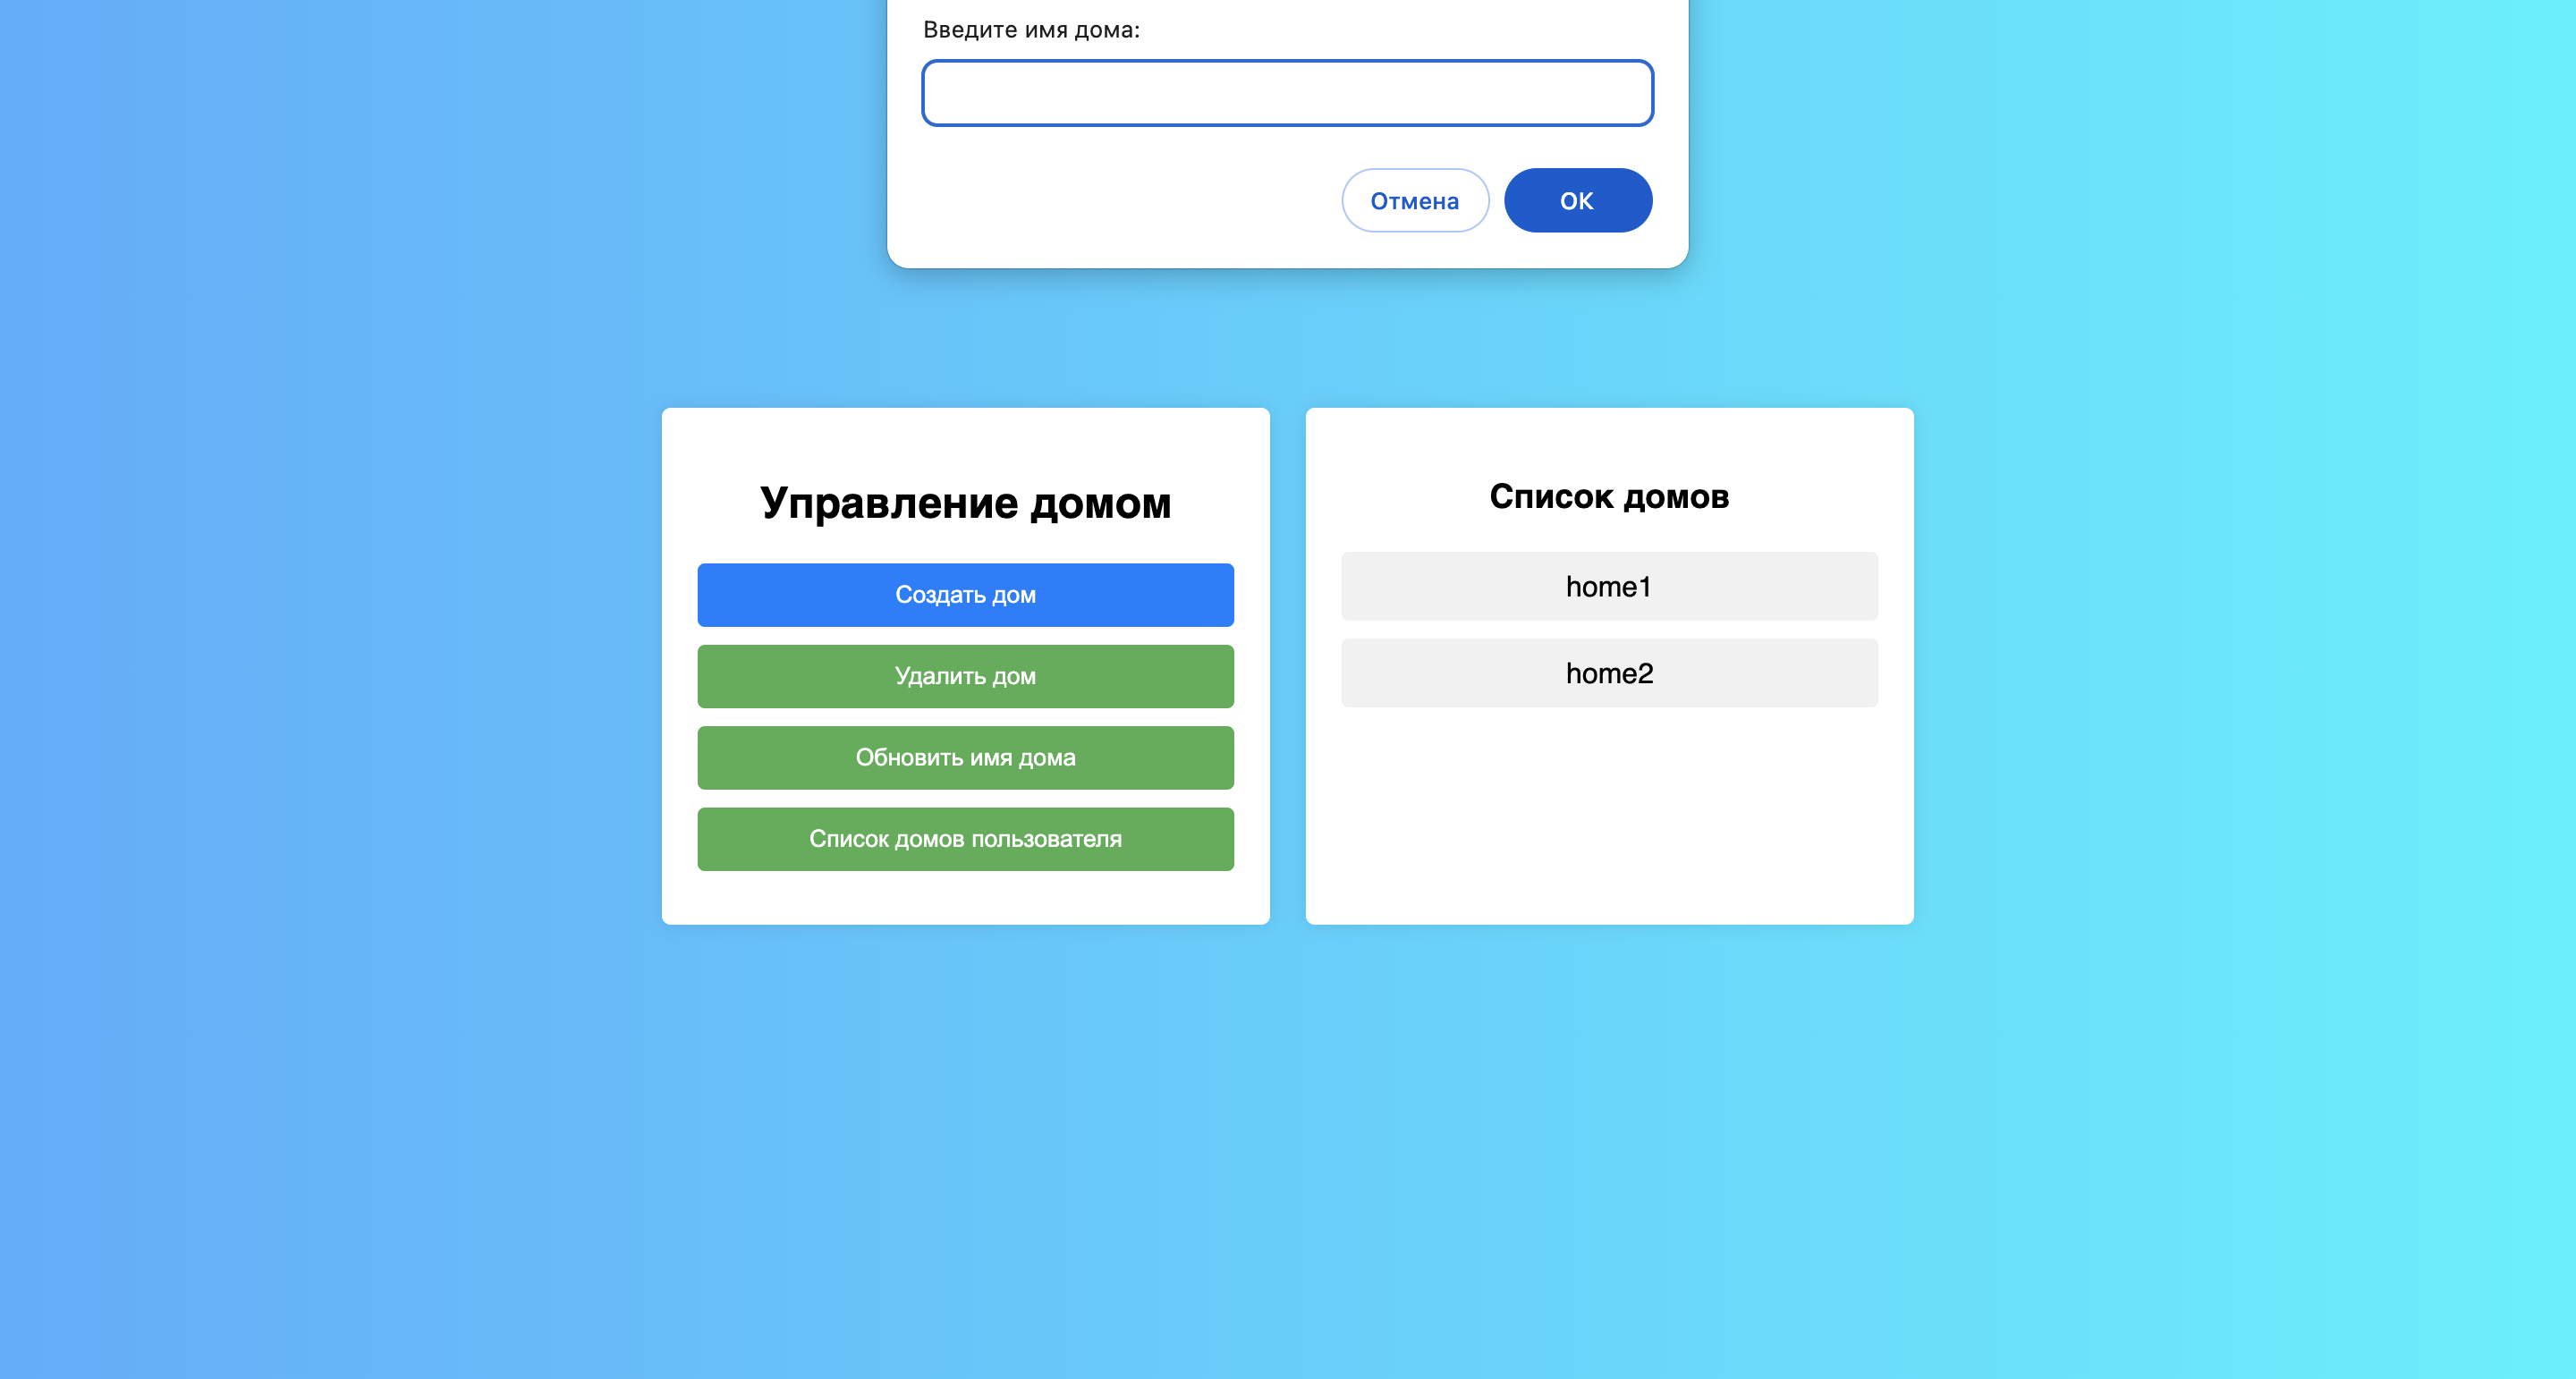
\includegraphics[width=1\linewidth]{img/home.png}
    \caption{\label{img:home} Страница для управления домом}
\end{figure}
\noindent

При нажатии на кнопку «Привилегии доступа» пользователь переходит на страницу, которая предоставляет возможность
управлять многопользовательским режимом \ref{img:access}. На данной странцие владелец дома может
добавить новых участников или удалить их. Также ему предоставляется возможность
просмотреть список участников дома и обновить уровень доступа участника.

\begin{figure}[H]
    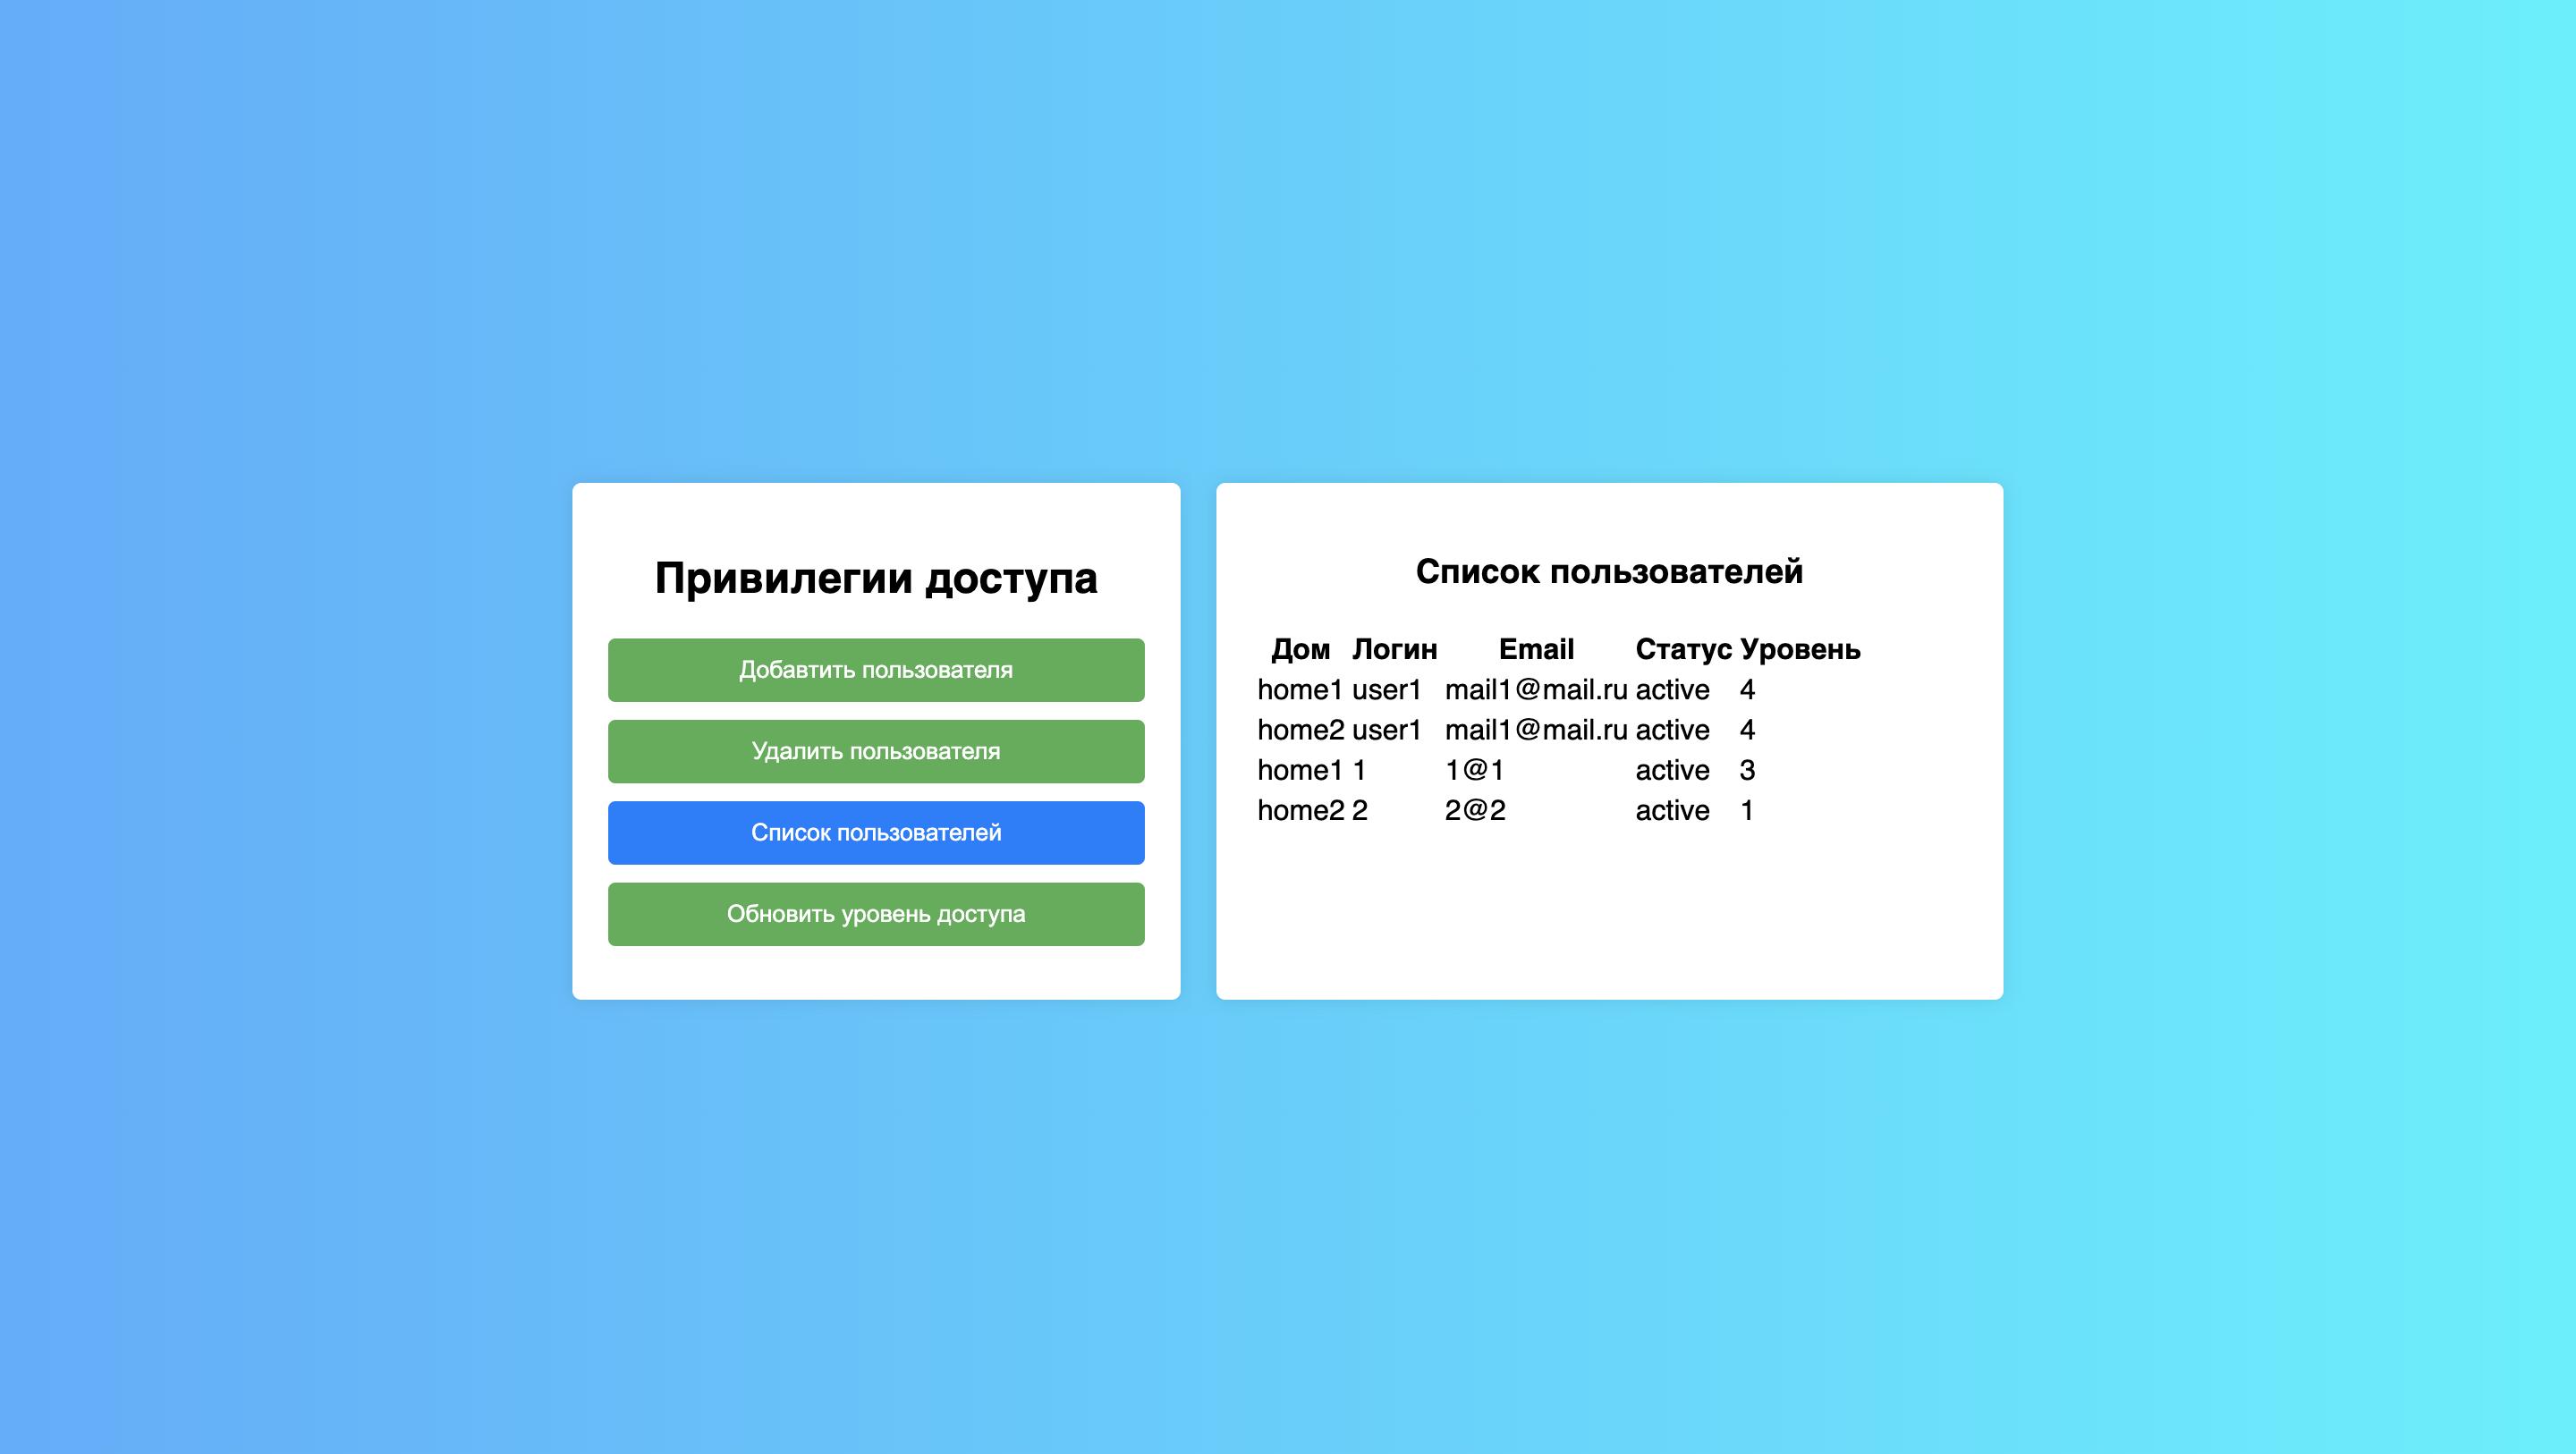
\includegraphics[width=1\linewidth]{img/access.png}
    \caption{\label{img:access} Страница многопользовательского режима}
\end{figure}
\noindent

При нажатии на кнопу «Устройство» пользователь переходит на страницу управления устройствами \ref{img:dev}. На данной странице 
пользователь может добавить новое устройство в свой дом или удалить уже добавленное. Также ему предоставляется возможность
просмотреть список устройств, запустить устройство и просмотреть историю работы устройства.

\begin{figure}[H]
    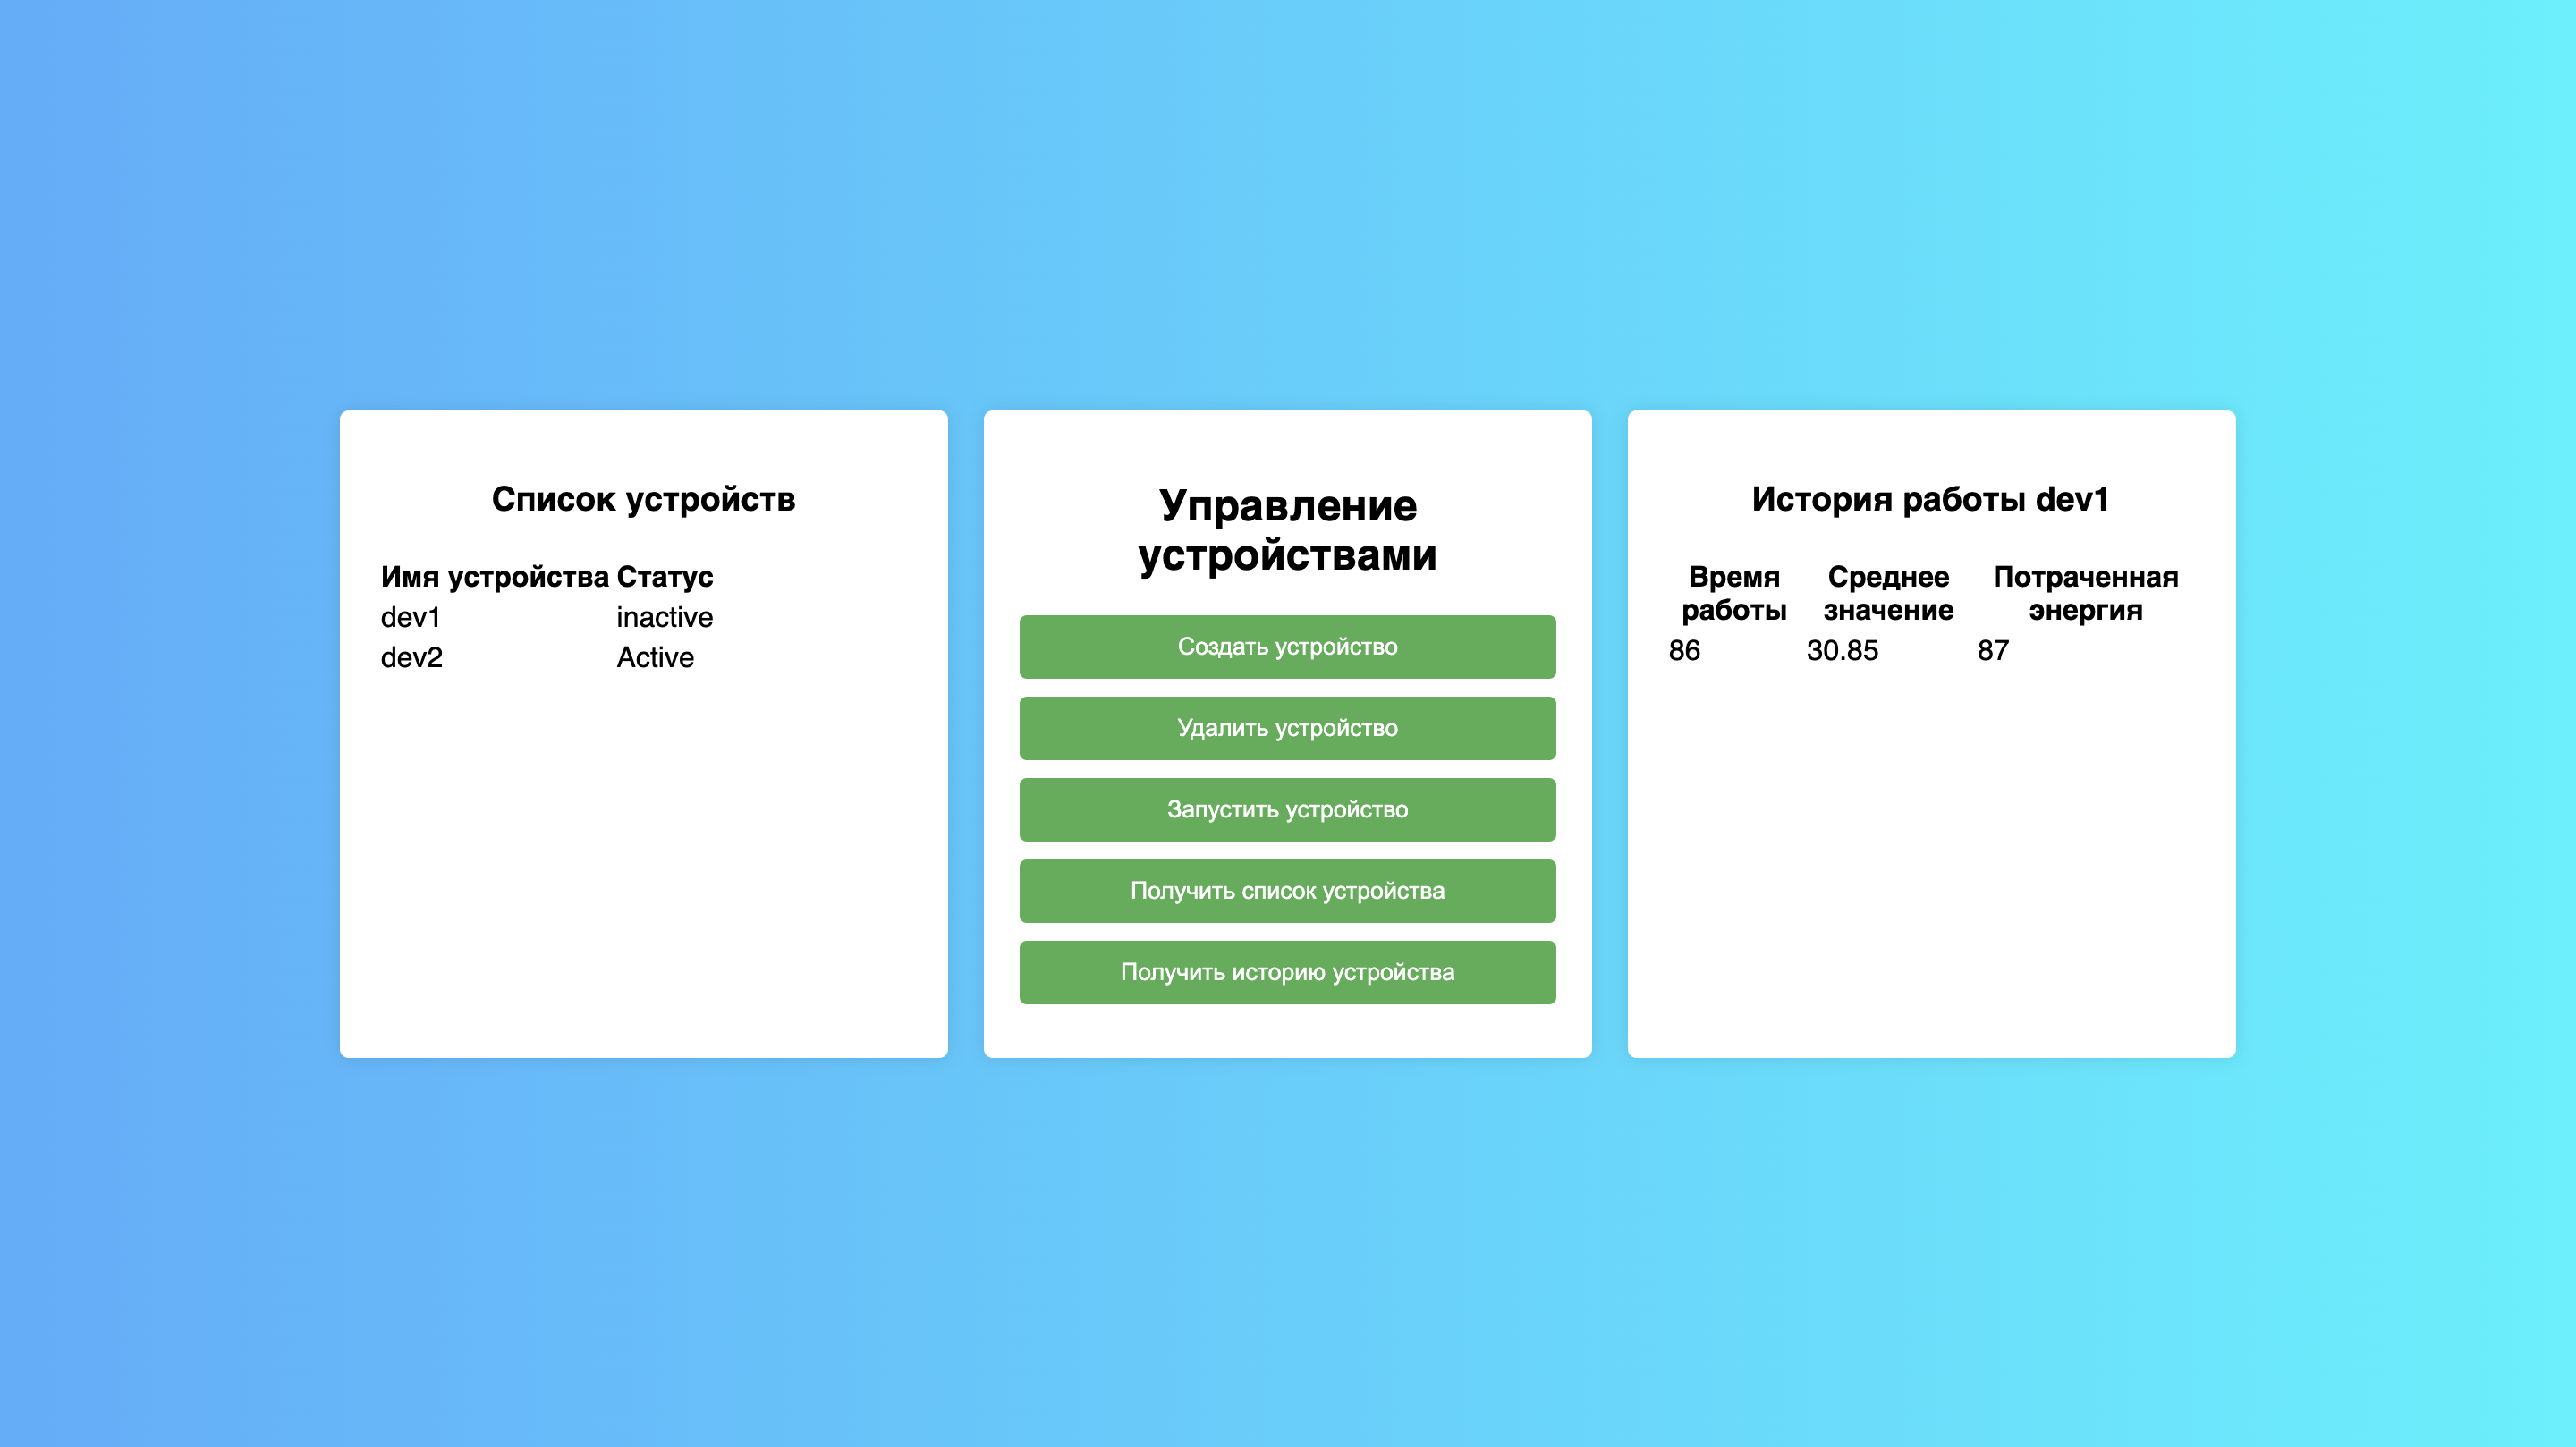
\includegraphics[width=1\linewidth]{img/device.png}
    \caption{\label{img:dev} Страница управления устройством}
\end{figure}
\noindent

\section*{Вывод}

В данном разделе был проведен выбор системы базы данных, а также
были выбраны средства реализации и среда разработки. Также было произведено тестрирование 
описанной ранее функции и запросов, выполняемых к базе данных, описан интерфейс приложения.

    \chapter*{Исследовательская часть}

В данном разделе представлены результаты исследования, которое заключалось в нахождении
зависимости времени выполнения запроса с использованием индексов и без, а так же технические 
характеристики устройства, на котором данное исследование было сделано.

\section{Технические характеристики}

Исследование было выполнено на устройстве, 
которое имеет следующие характеристики:

\begin{itemize}
    \item операционная система macOS Sonoma 14.1.1 [14];
    \item 2 GHz 4-ядерный процессор Intel Core i5
    \item оперативная память: 16 Гб.
\end{itemize}

\section{Исследование времени выполнения запроса от наличия индексов}



    \chapter*{Заключение}
\addcontentsline{toc}{chapter}{Заключение}

Цель курсовой работы, которая заключалась в разработке базы данных 
для IoT-платформы умный дом, достигнтуа.
Так же были выполнены следующие задачи:

\begin{itemize}[left=\parindent]
    \item проведен анализ существующих решений;
    \item сформулированы требования к разрабатываемой базе данных;
    \item проанализированы существующие базы данных на основе данной задачи;
    \item спроектирована и разработана база данных;
    \item спроектировано и разработано приложение для взаимодействия с базой данных;
    \item проведено исследование зависимости времени выполнения запросов
    с использованием индексов и без.
\end{itemize}


    \makebibliography

    \chapter*{Приложение А}
\addcontentsline{toc}{chapter}{Приложение А}

\includelistingpretty
{list1.sql}
{sql}
{Реализация функции, используемой для смены статуса устройства в соответствии с текущим состоянием}

    \chapter*{Приложение Б}
\addcontentsline{toc}{chapter}{Приложение Б}

\includelistingpretty
{list2.sql}
{sql}
{Создание роли гостя (неавторизованного пользователя)}

\includelistingpretty
{list3.sql}
{sql}
{Создание роли авторизованного пользователя}

\includelistingpretty
{list4.sql}
{sql}
{Создание роли владельца дома}
    \chapter*{Приложение В}
\addcontentsline{toc}{chapter}{Приложение В}

\begin{figure}[H]
    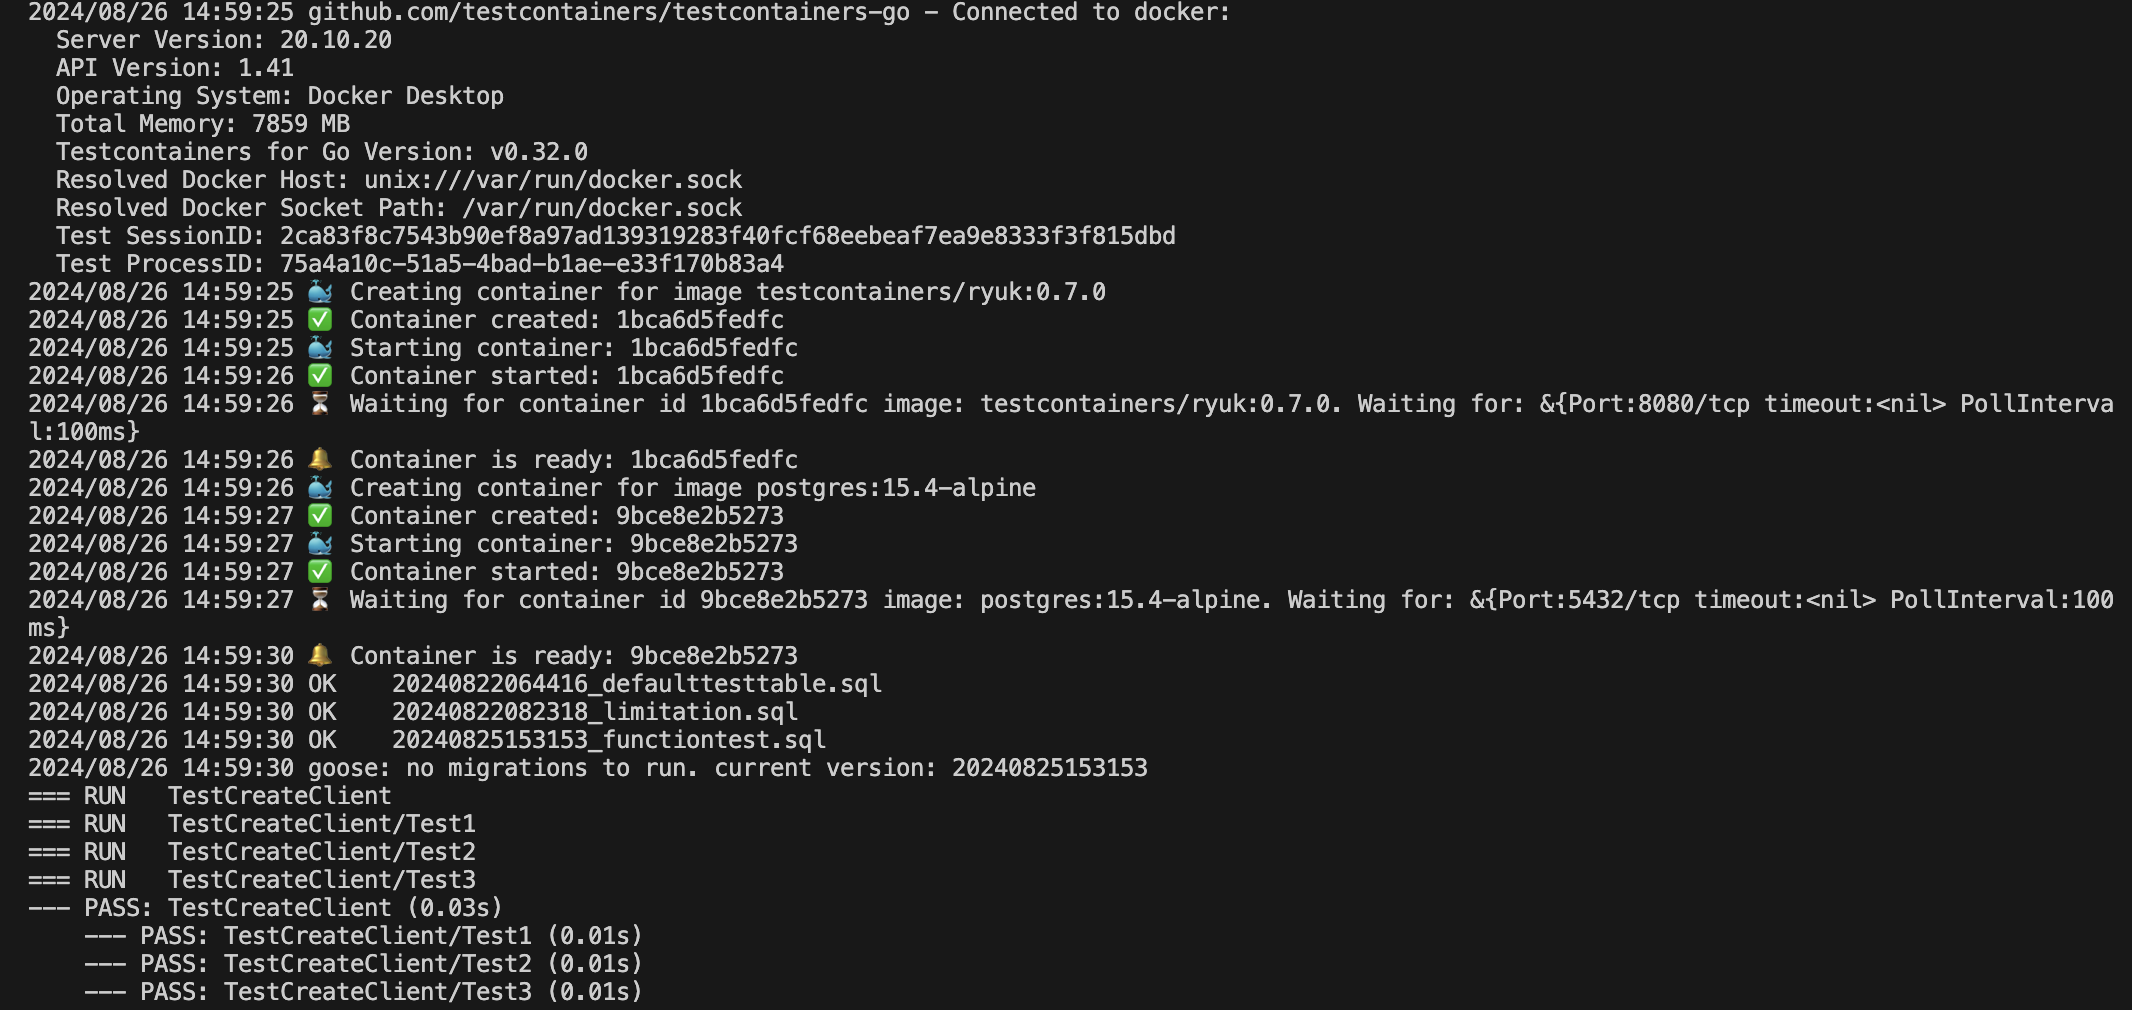
\includegraphics[width=1\linewidth]{./img/test2.png}
    \caption{\label{img:test1} Результаты тестирования работы запросов к базе данных}
\end{figure}
\noindent

\begin{figure}[H]
    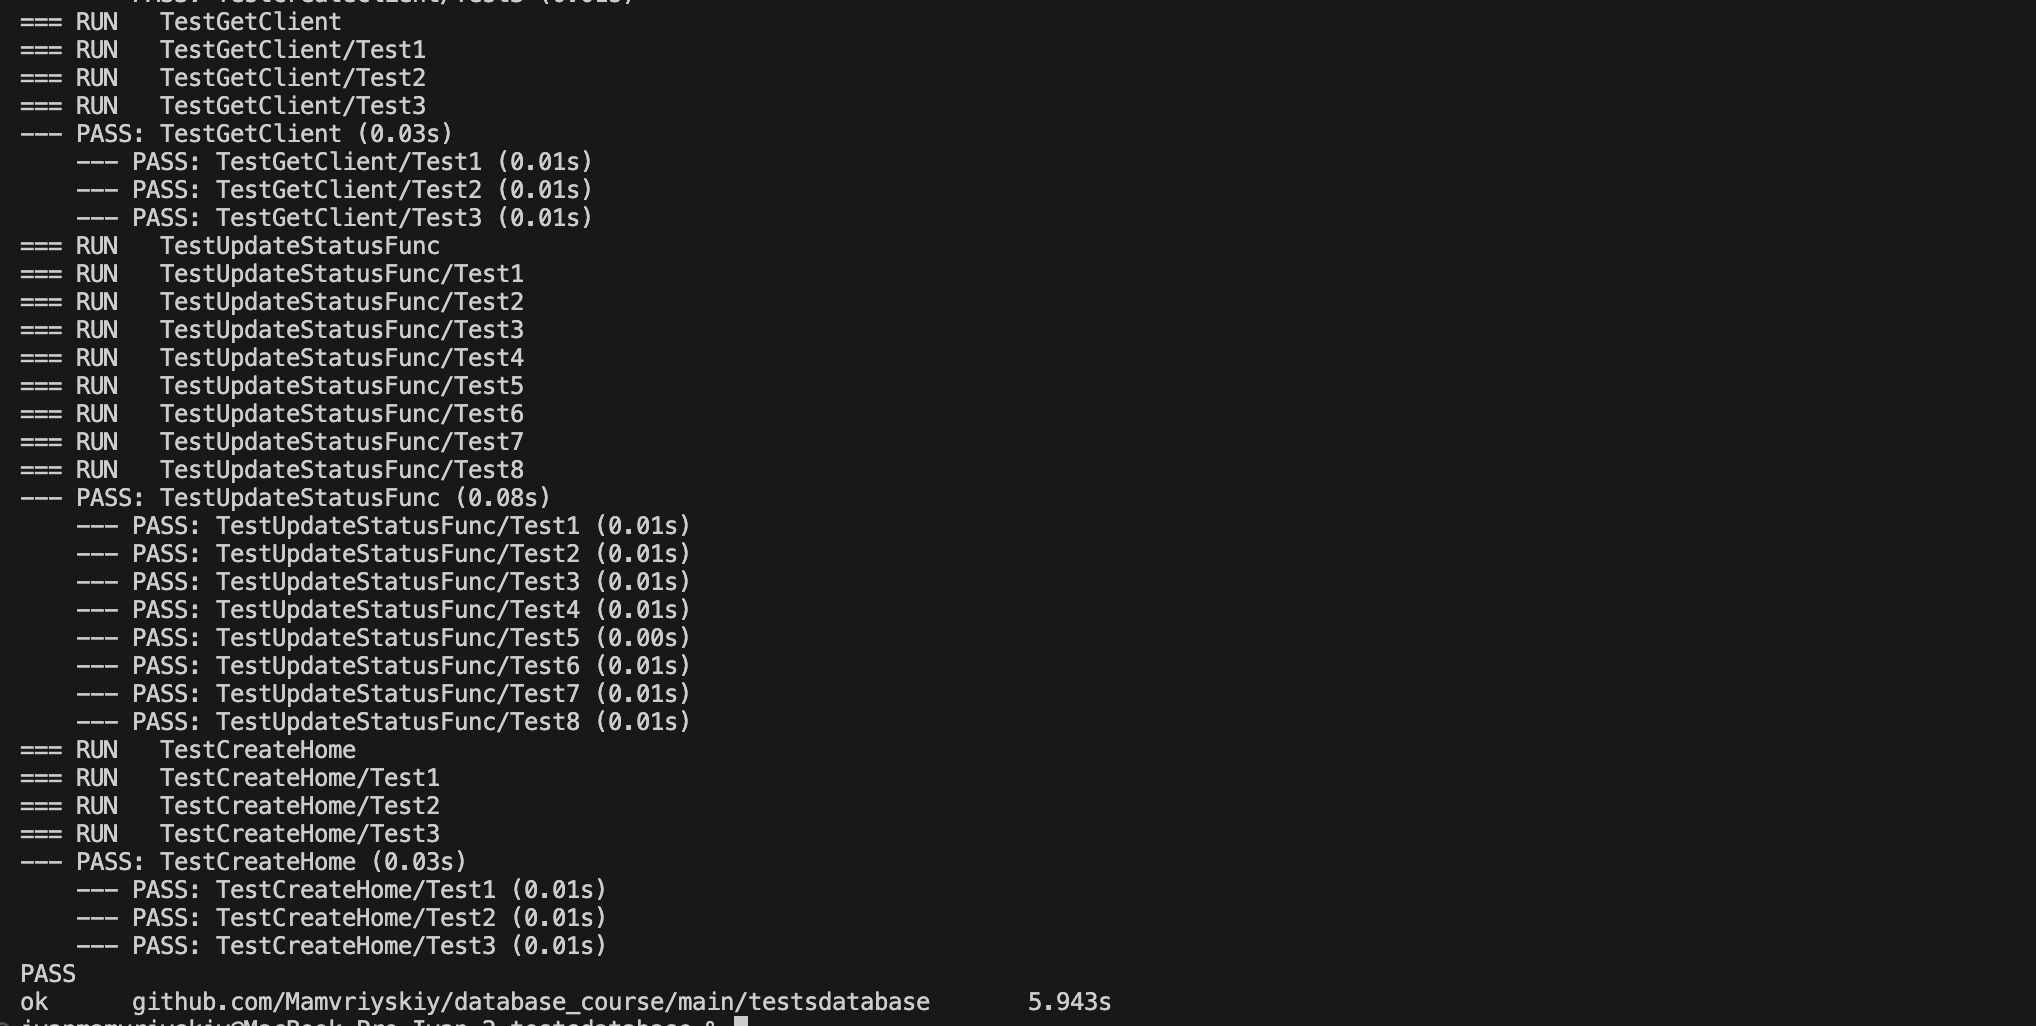
\includegraphics[width=1\linewidth]{./img/test1.png}
    \caption{\label{img:test2} Результаты тестирования работы запросов к базе данных}
\end{figure}
\noindent
    \chapter*{Приложение Г}
\addcontentsline{toc}{chapter}{Приложение Г}

\begin{figure}[H]
    
\includegraphics[width=1\linewidth]{img/1.png}
    \caption{Презентация -- слайд 1}
\end{figure}
\noindent

\begin{figure}[H]
    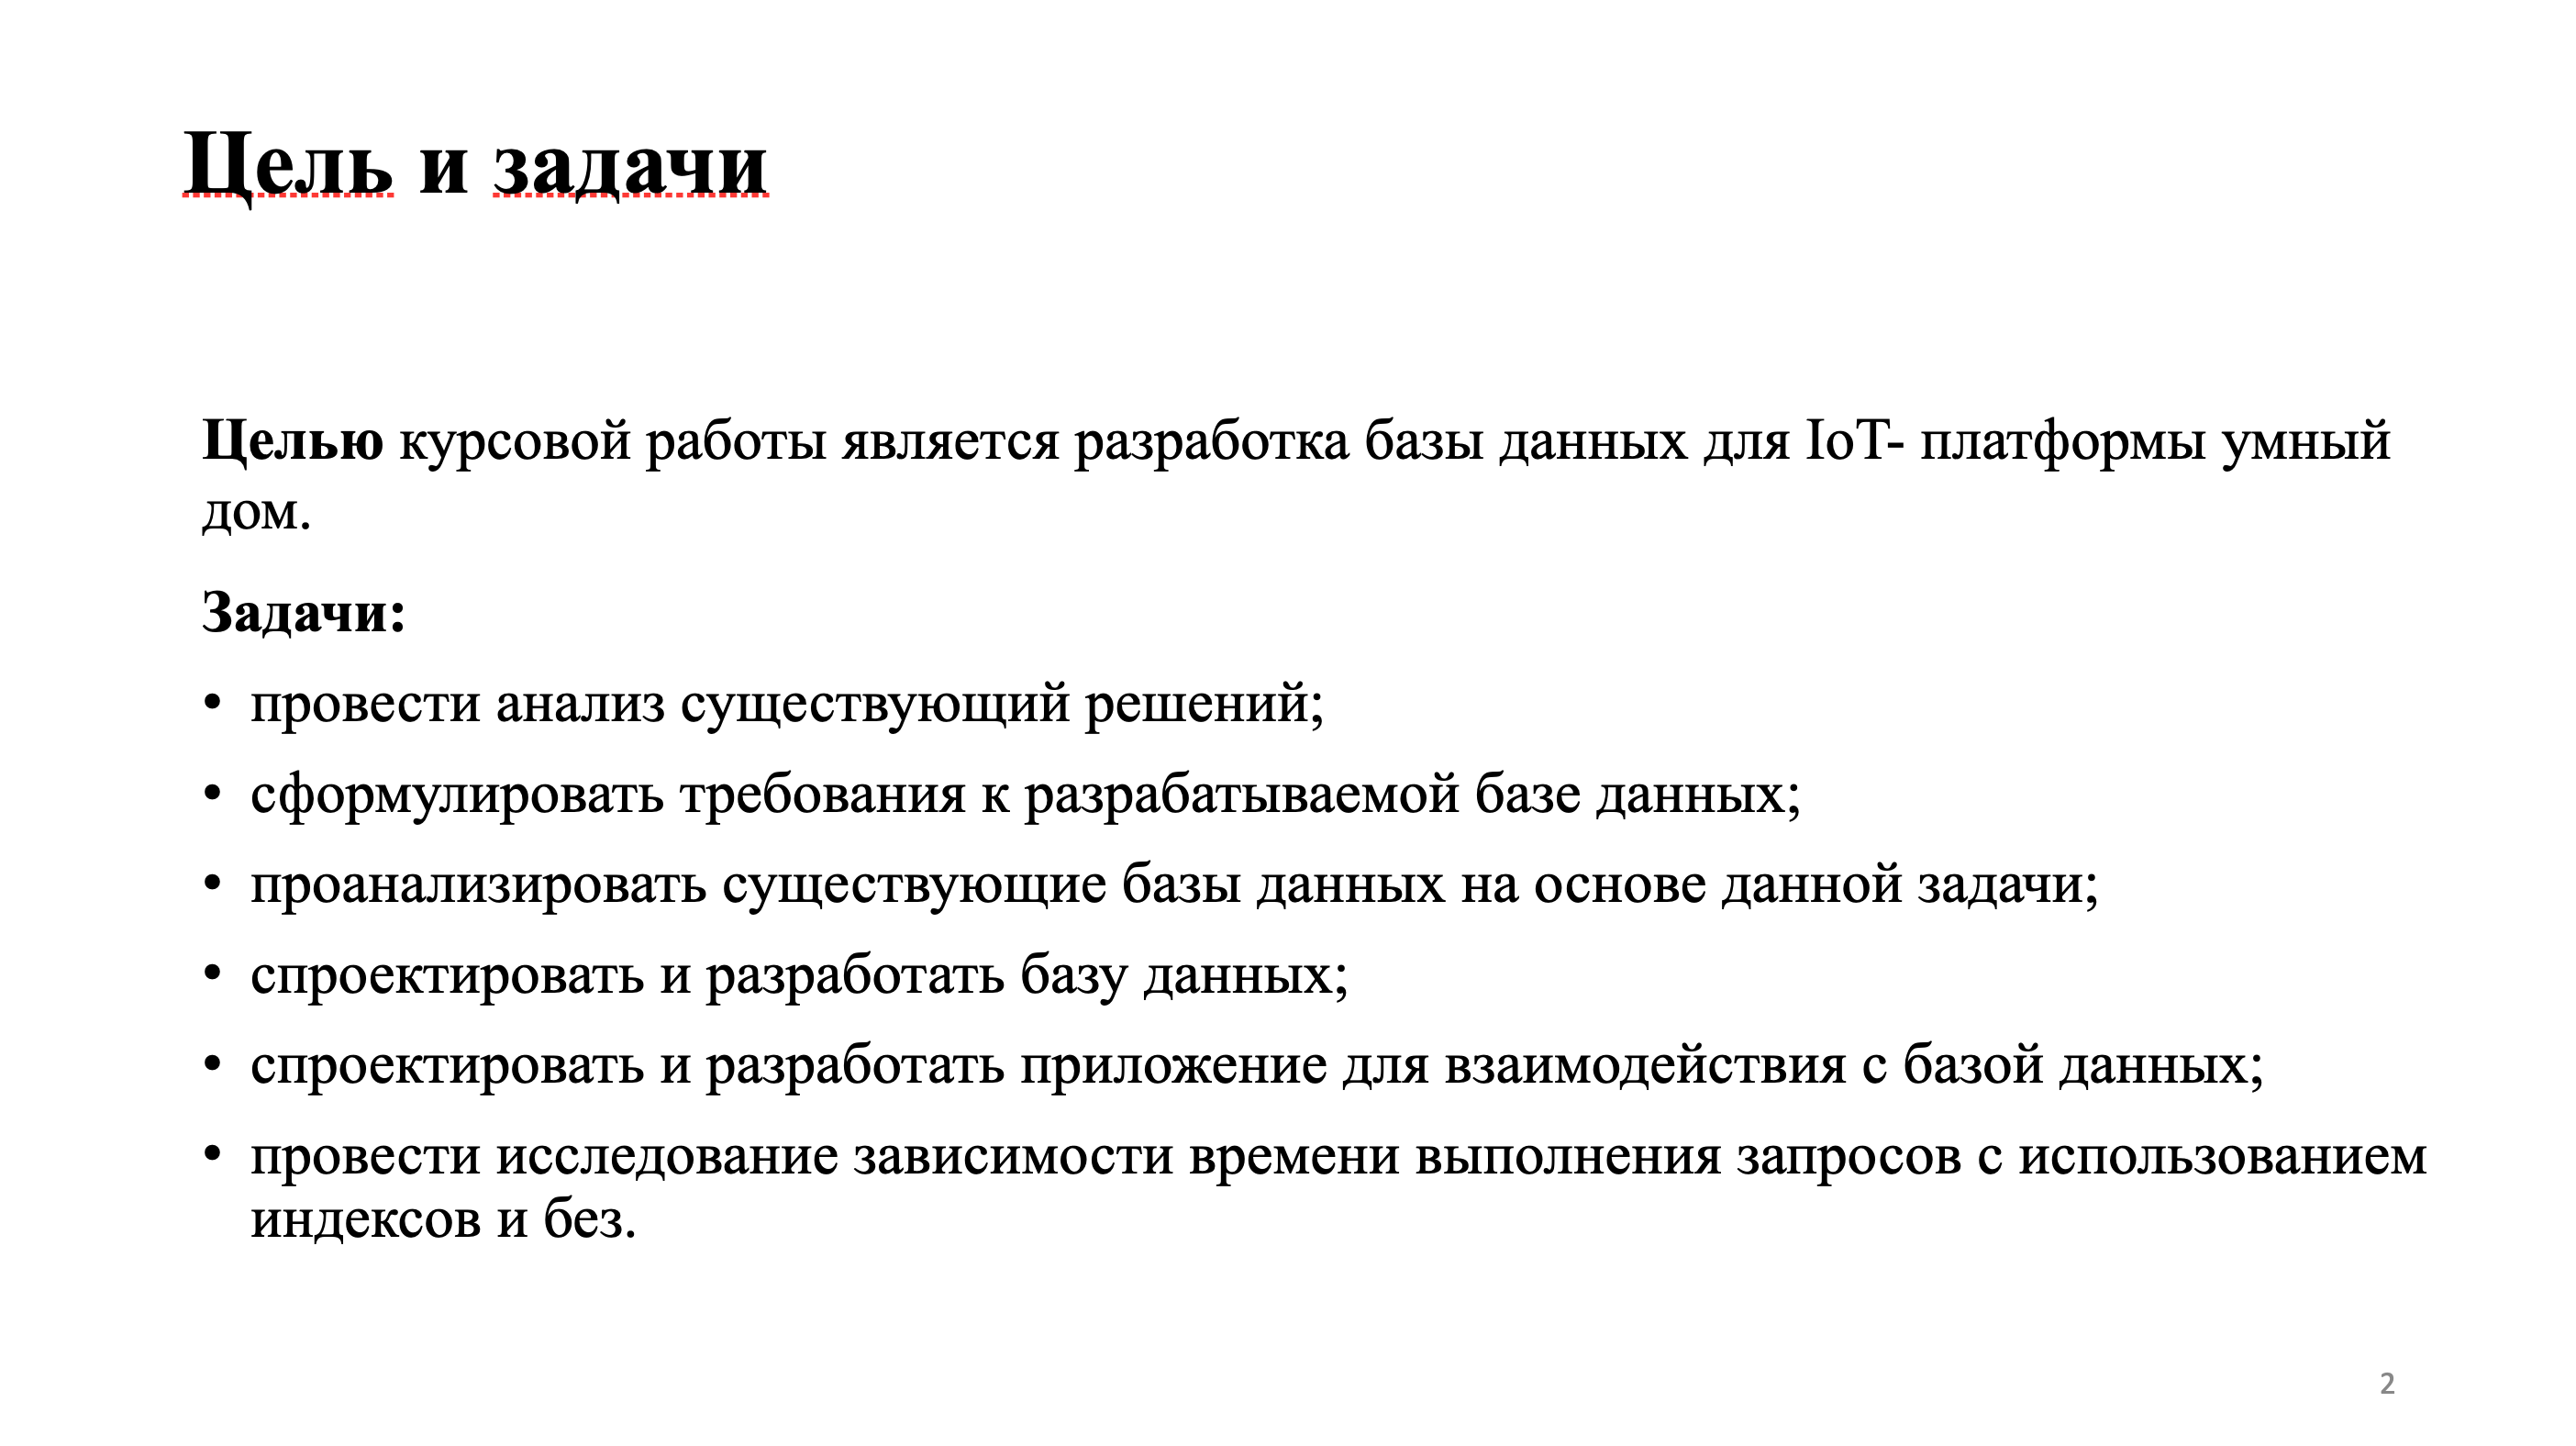
\includegraphics[width=1\linewidth]{img/2.png}
    \caption{Презентация -- слайд 2}
\end{figure}
\noindent

\begin{figure}[H]
    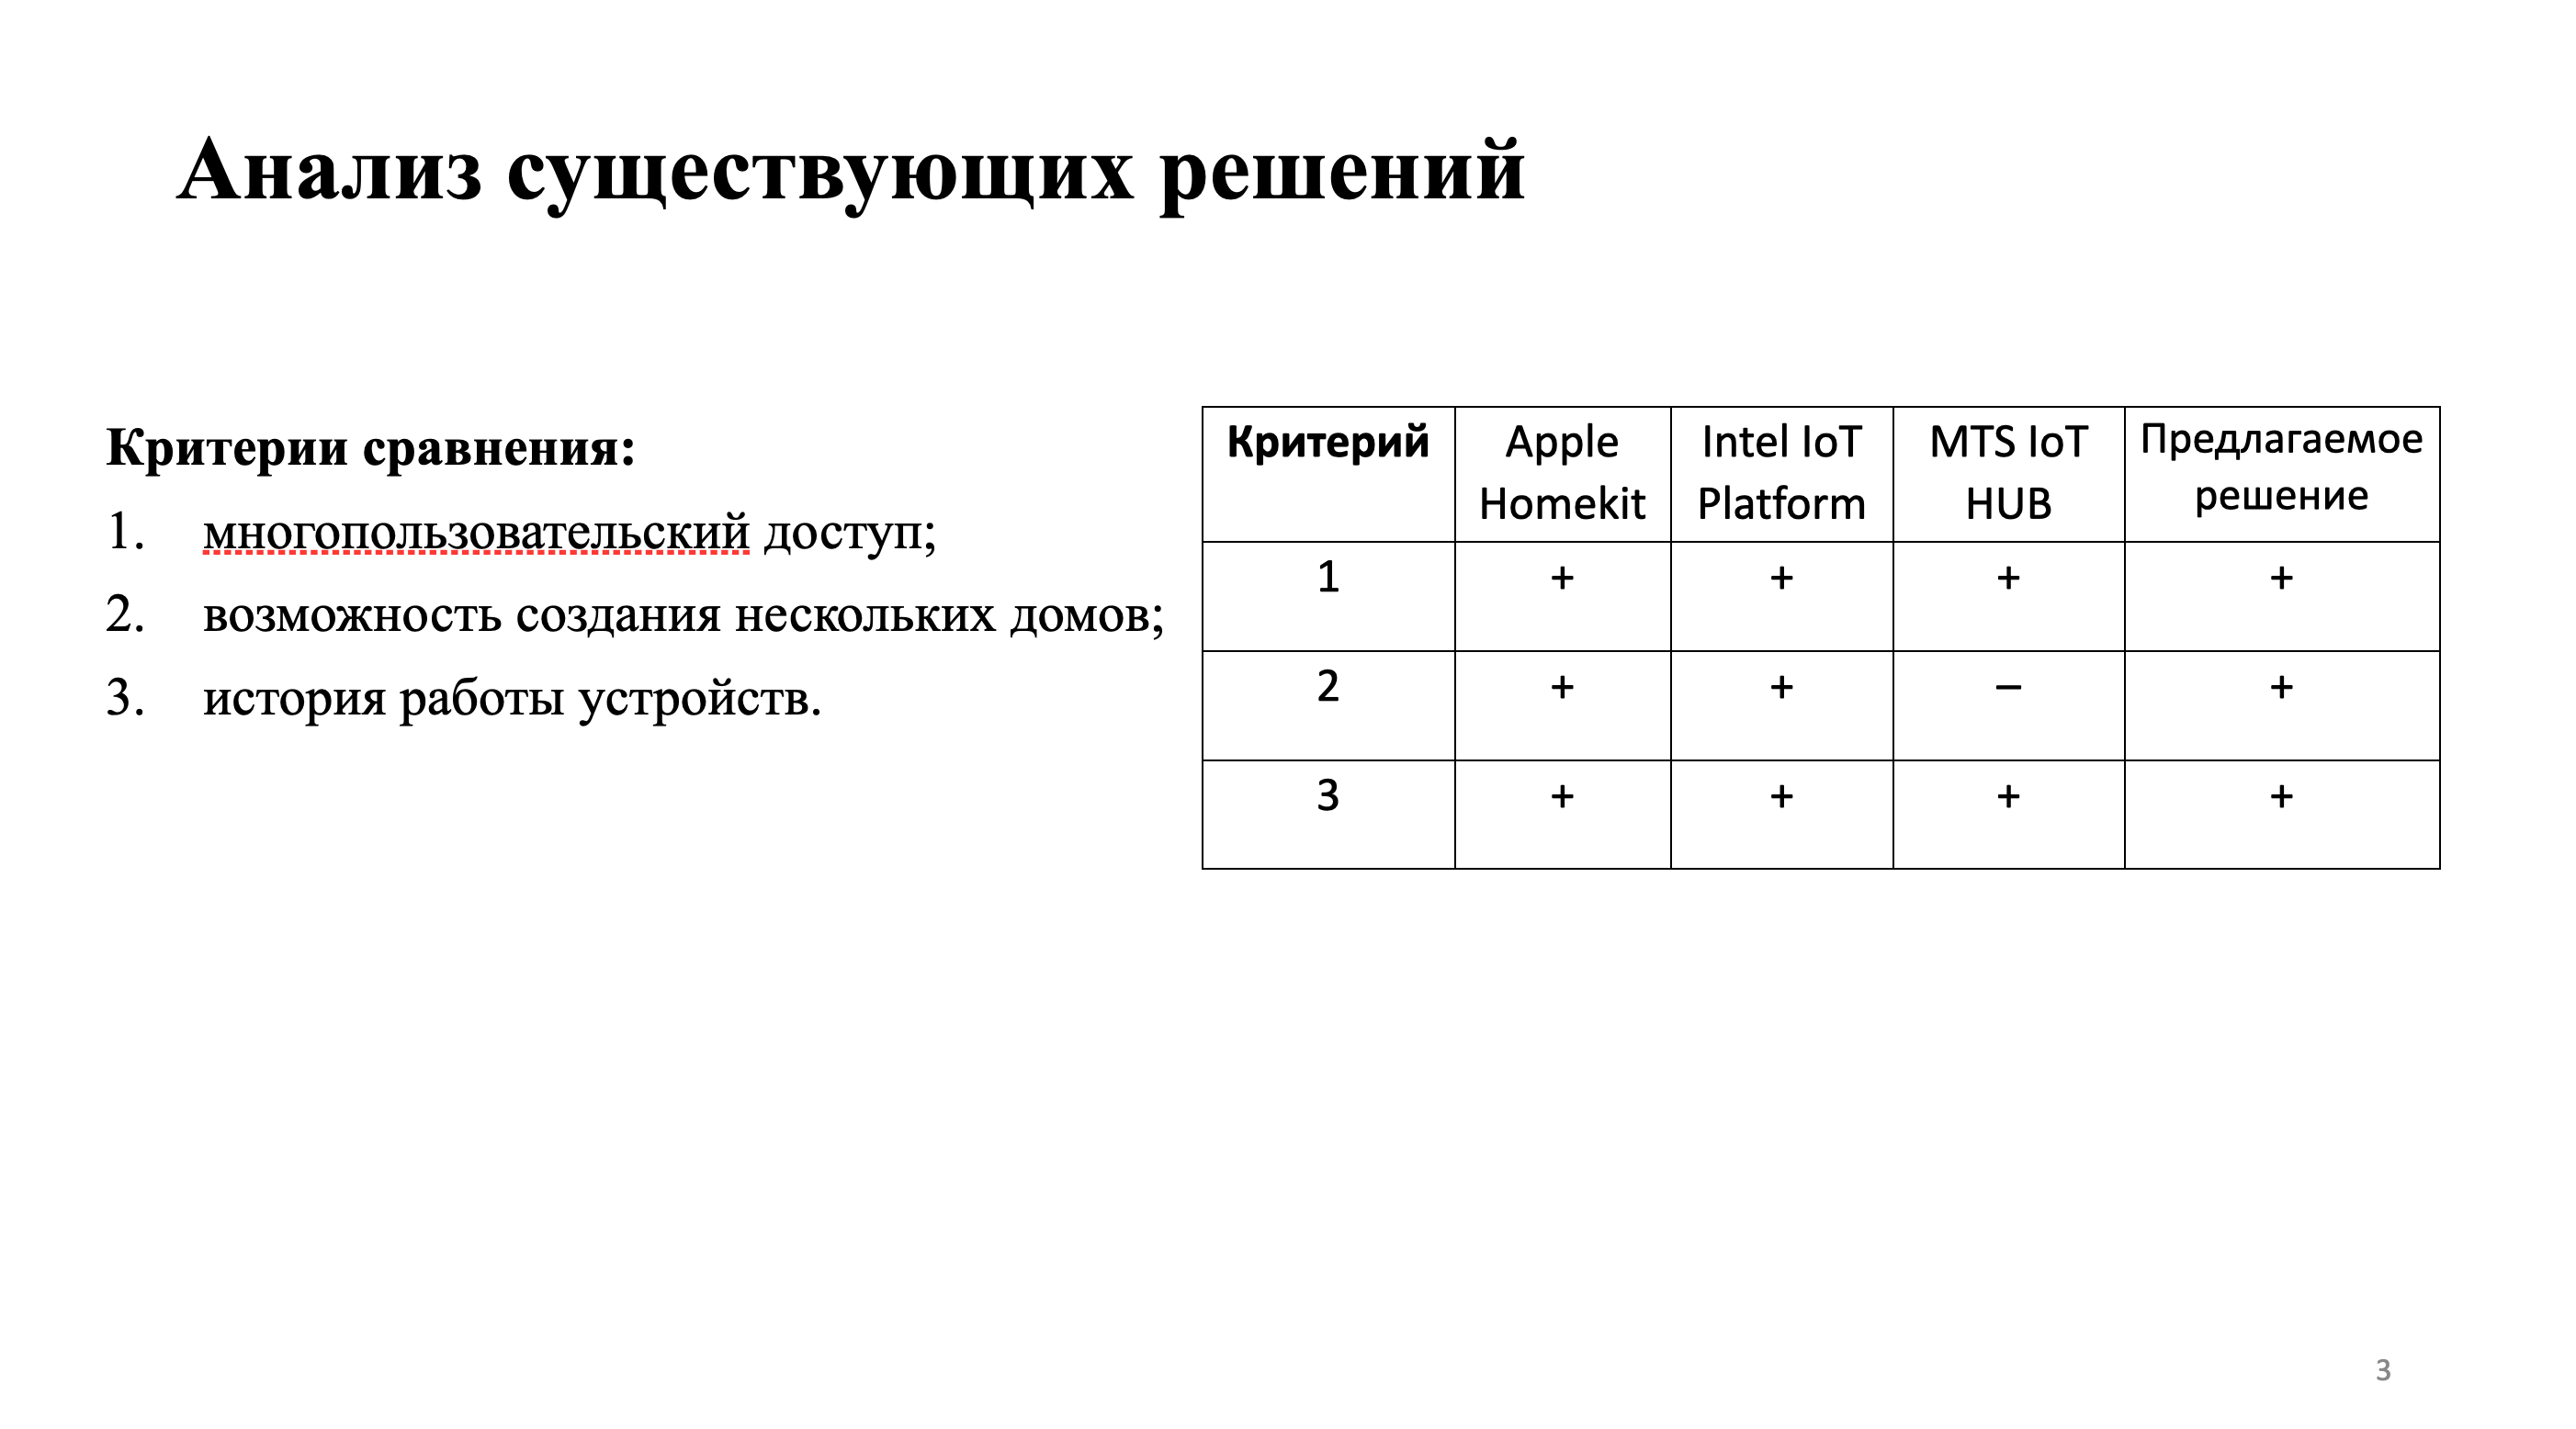
\includegraphics[width=1\linewidth]{img/3.png}
    \caption{Презентация -- слайд 3}
\end{figure}
\noindent

\begin{figure}[H]
    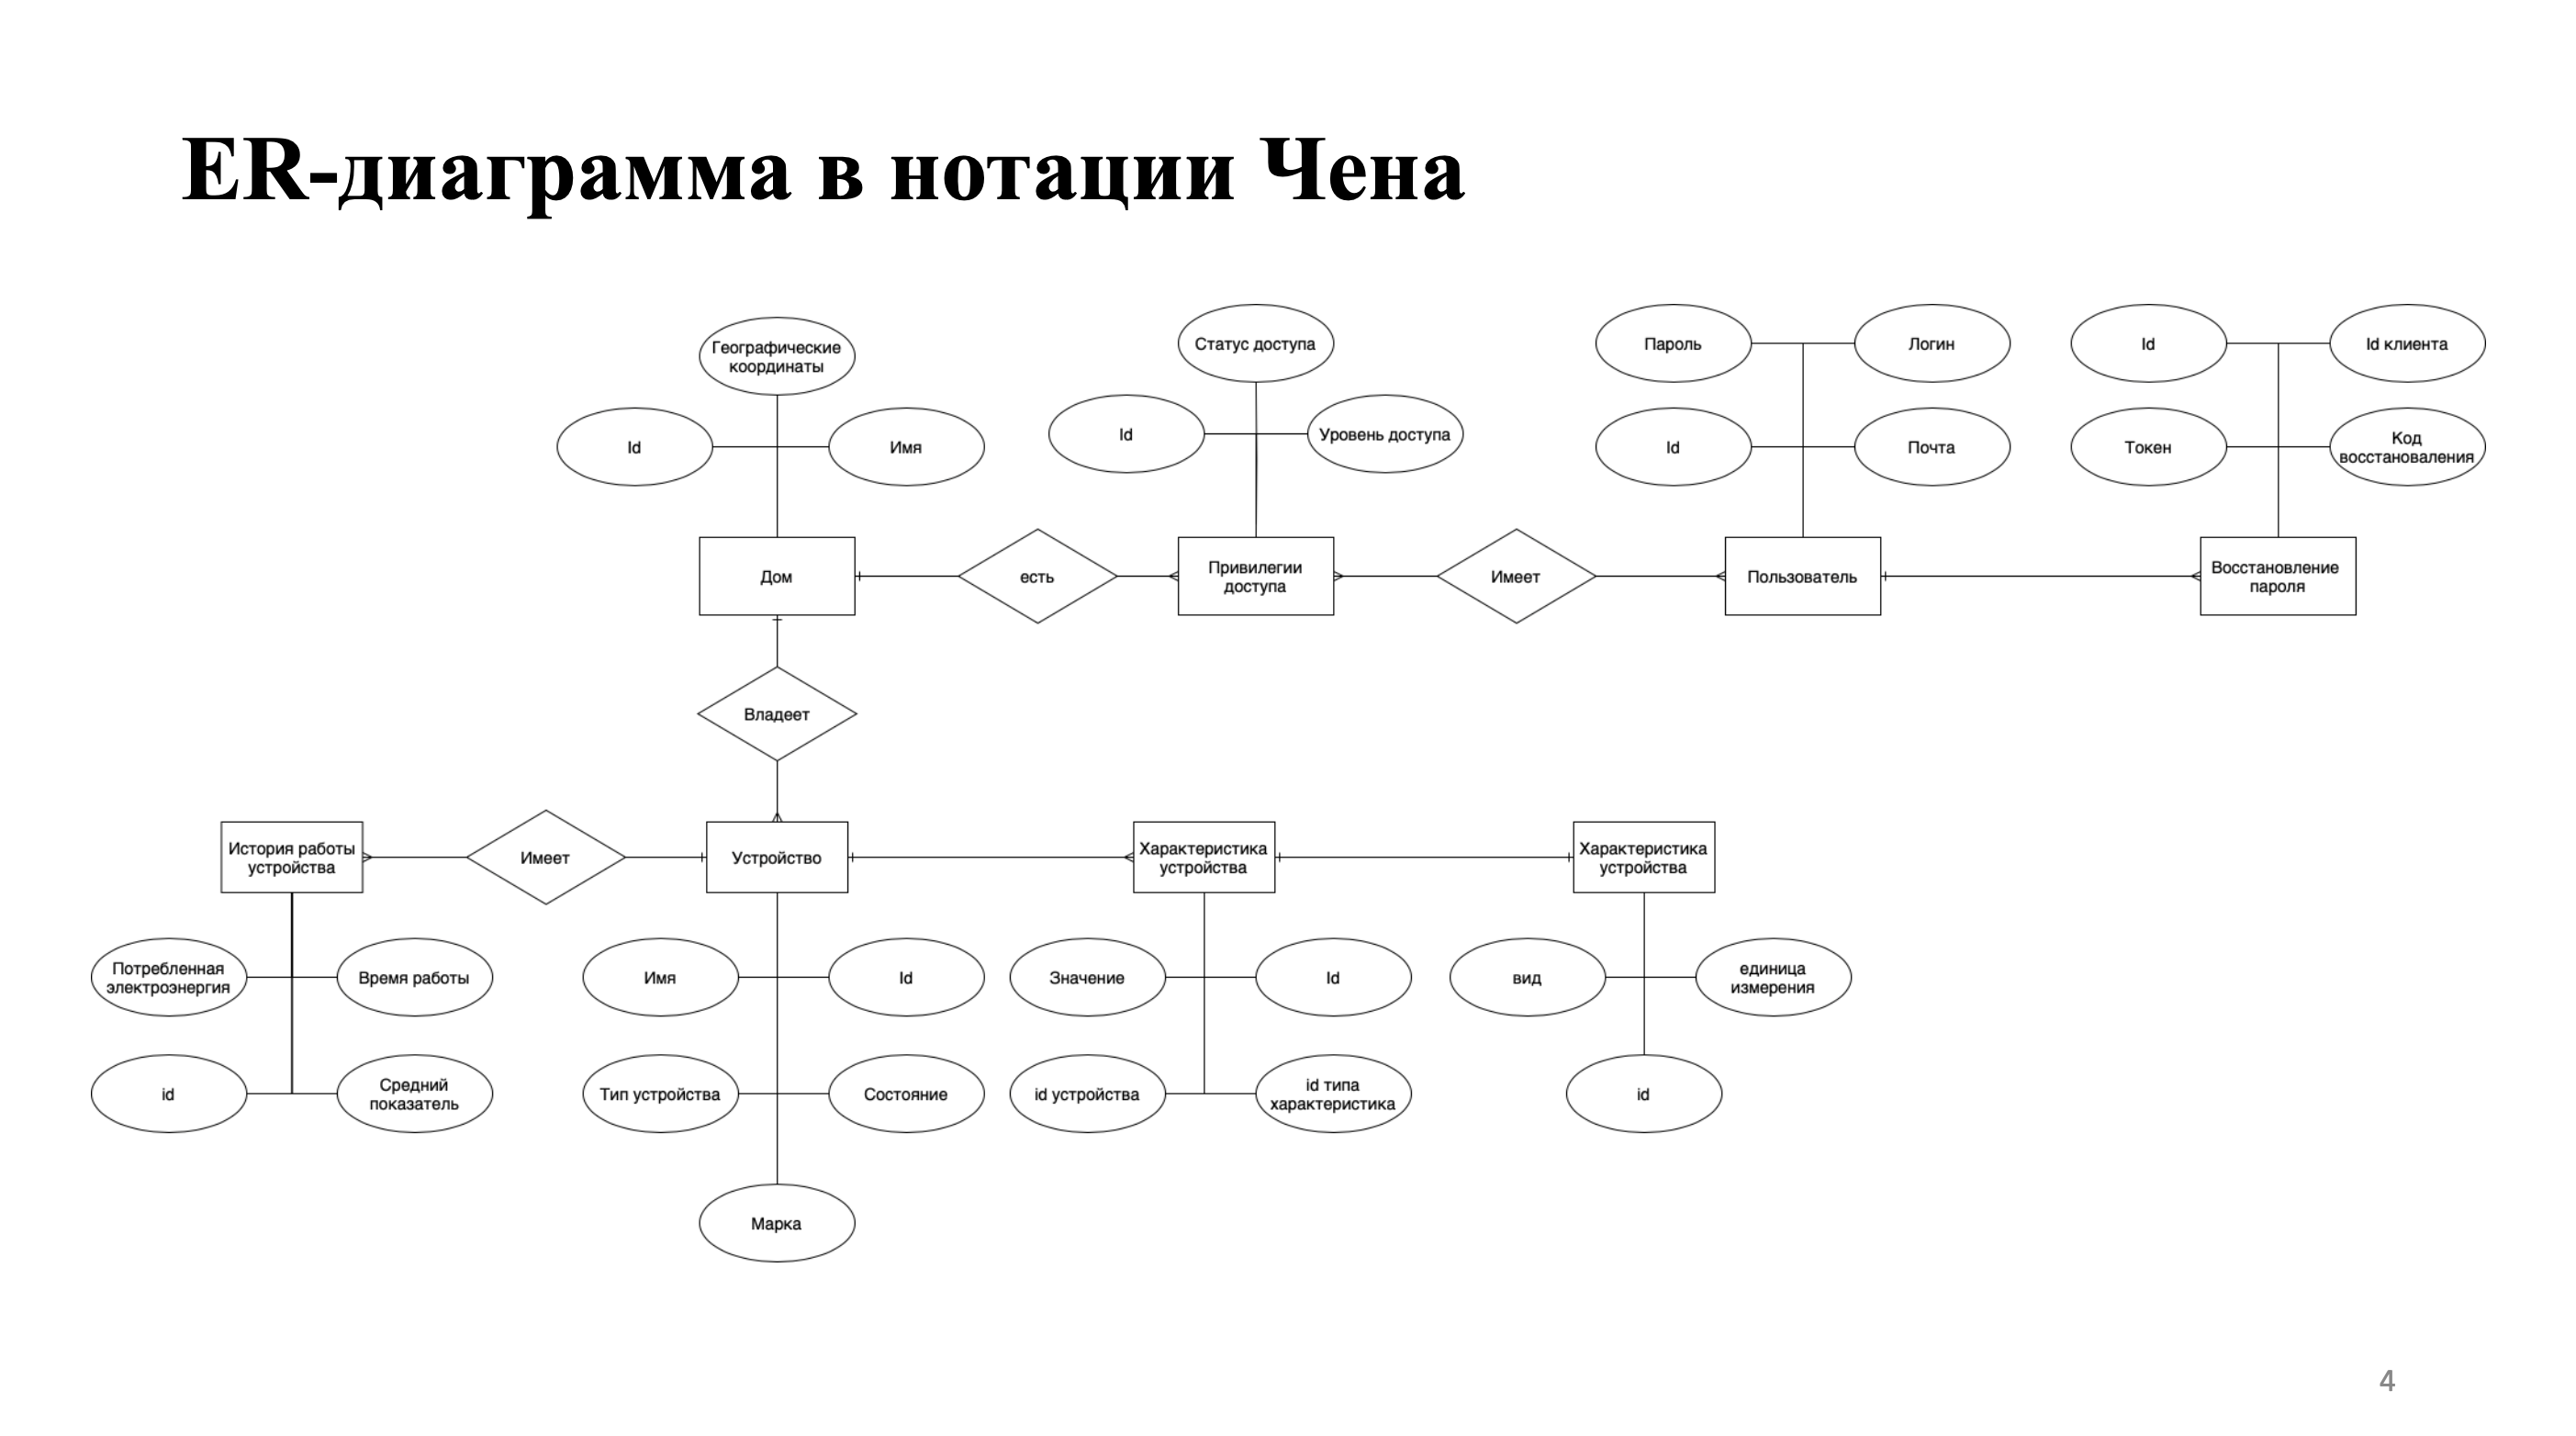
\includegraphics[width=1\linewidth]{img/4.png}
    \caption{Презентация -- слайд 4}
\end{figure}
\noindent

\begin{figure}[H]
    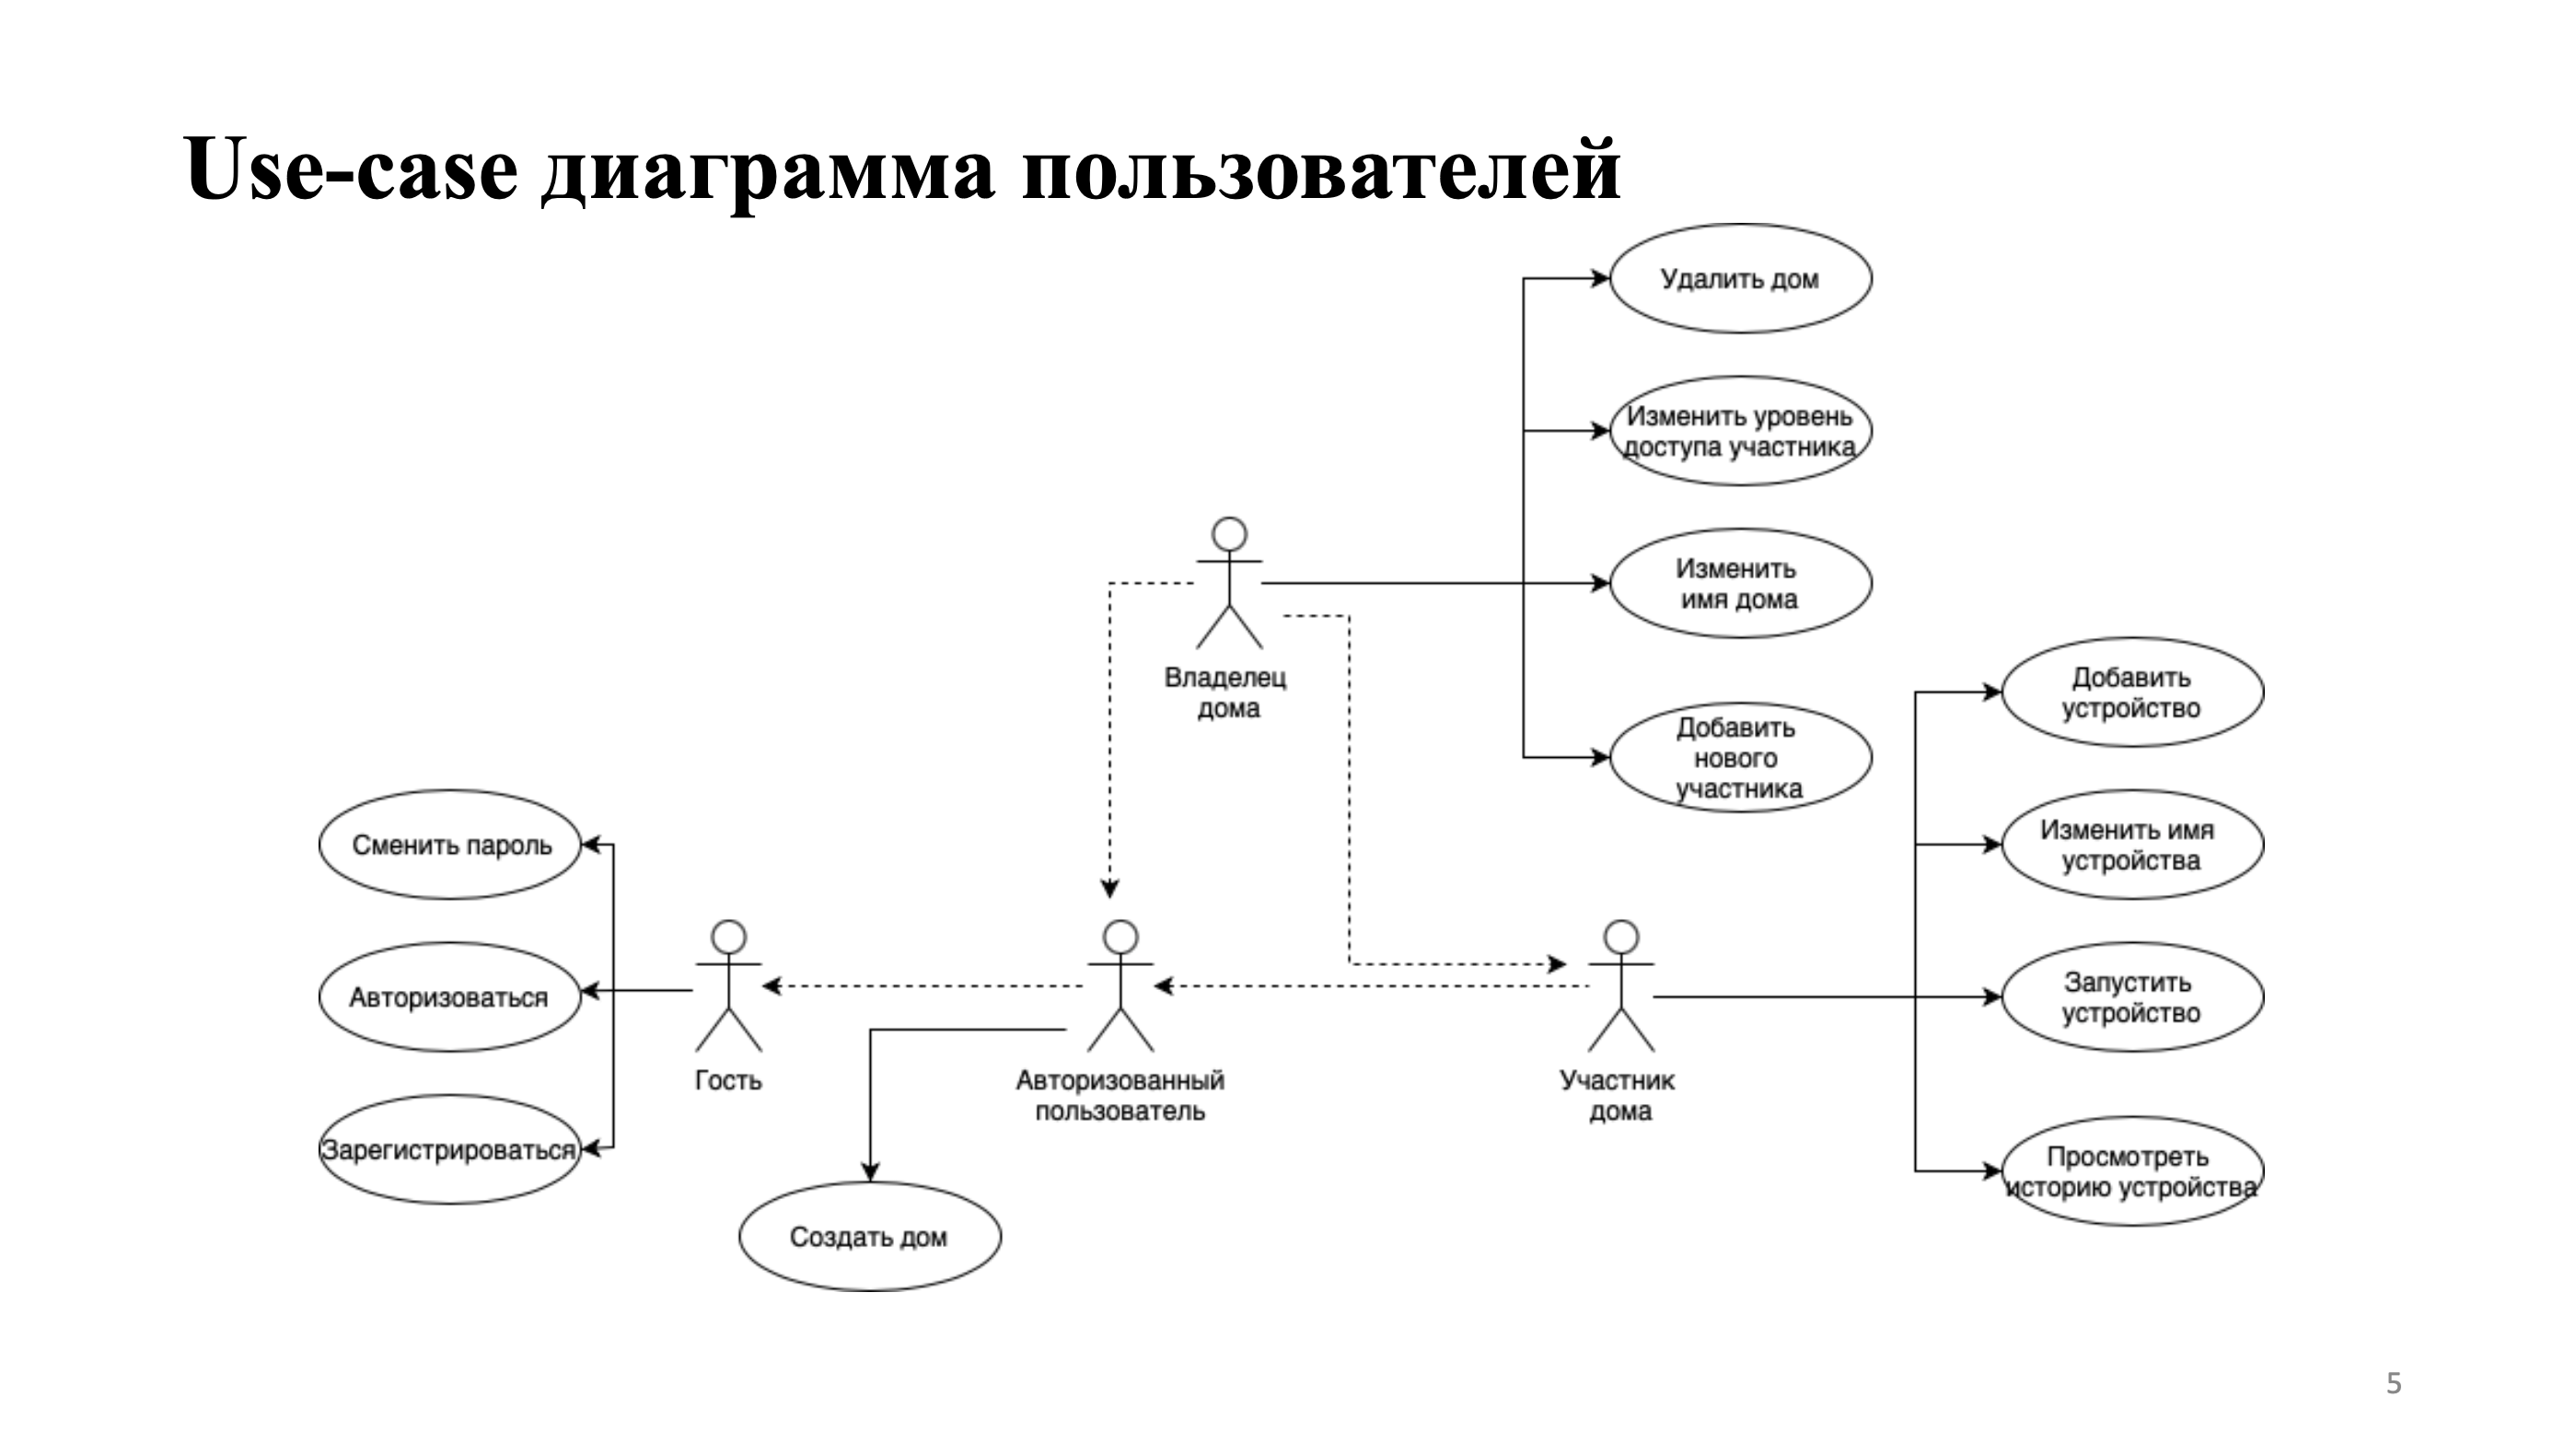
\includegraphics[width=1\linewidth]{img/5.png}
    \caption{Презентация -- слайд 5}
\end{figure}
\noindent

\begin{figure}[H]
    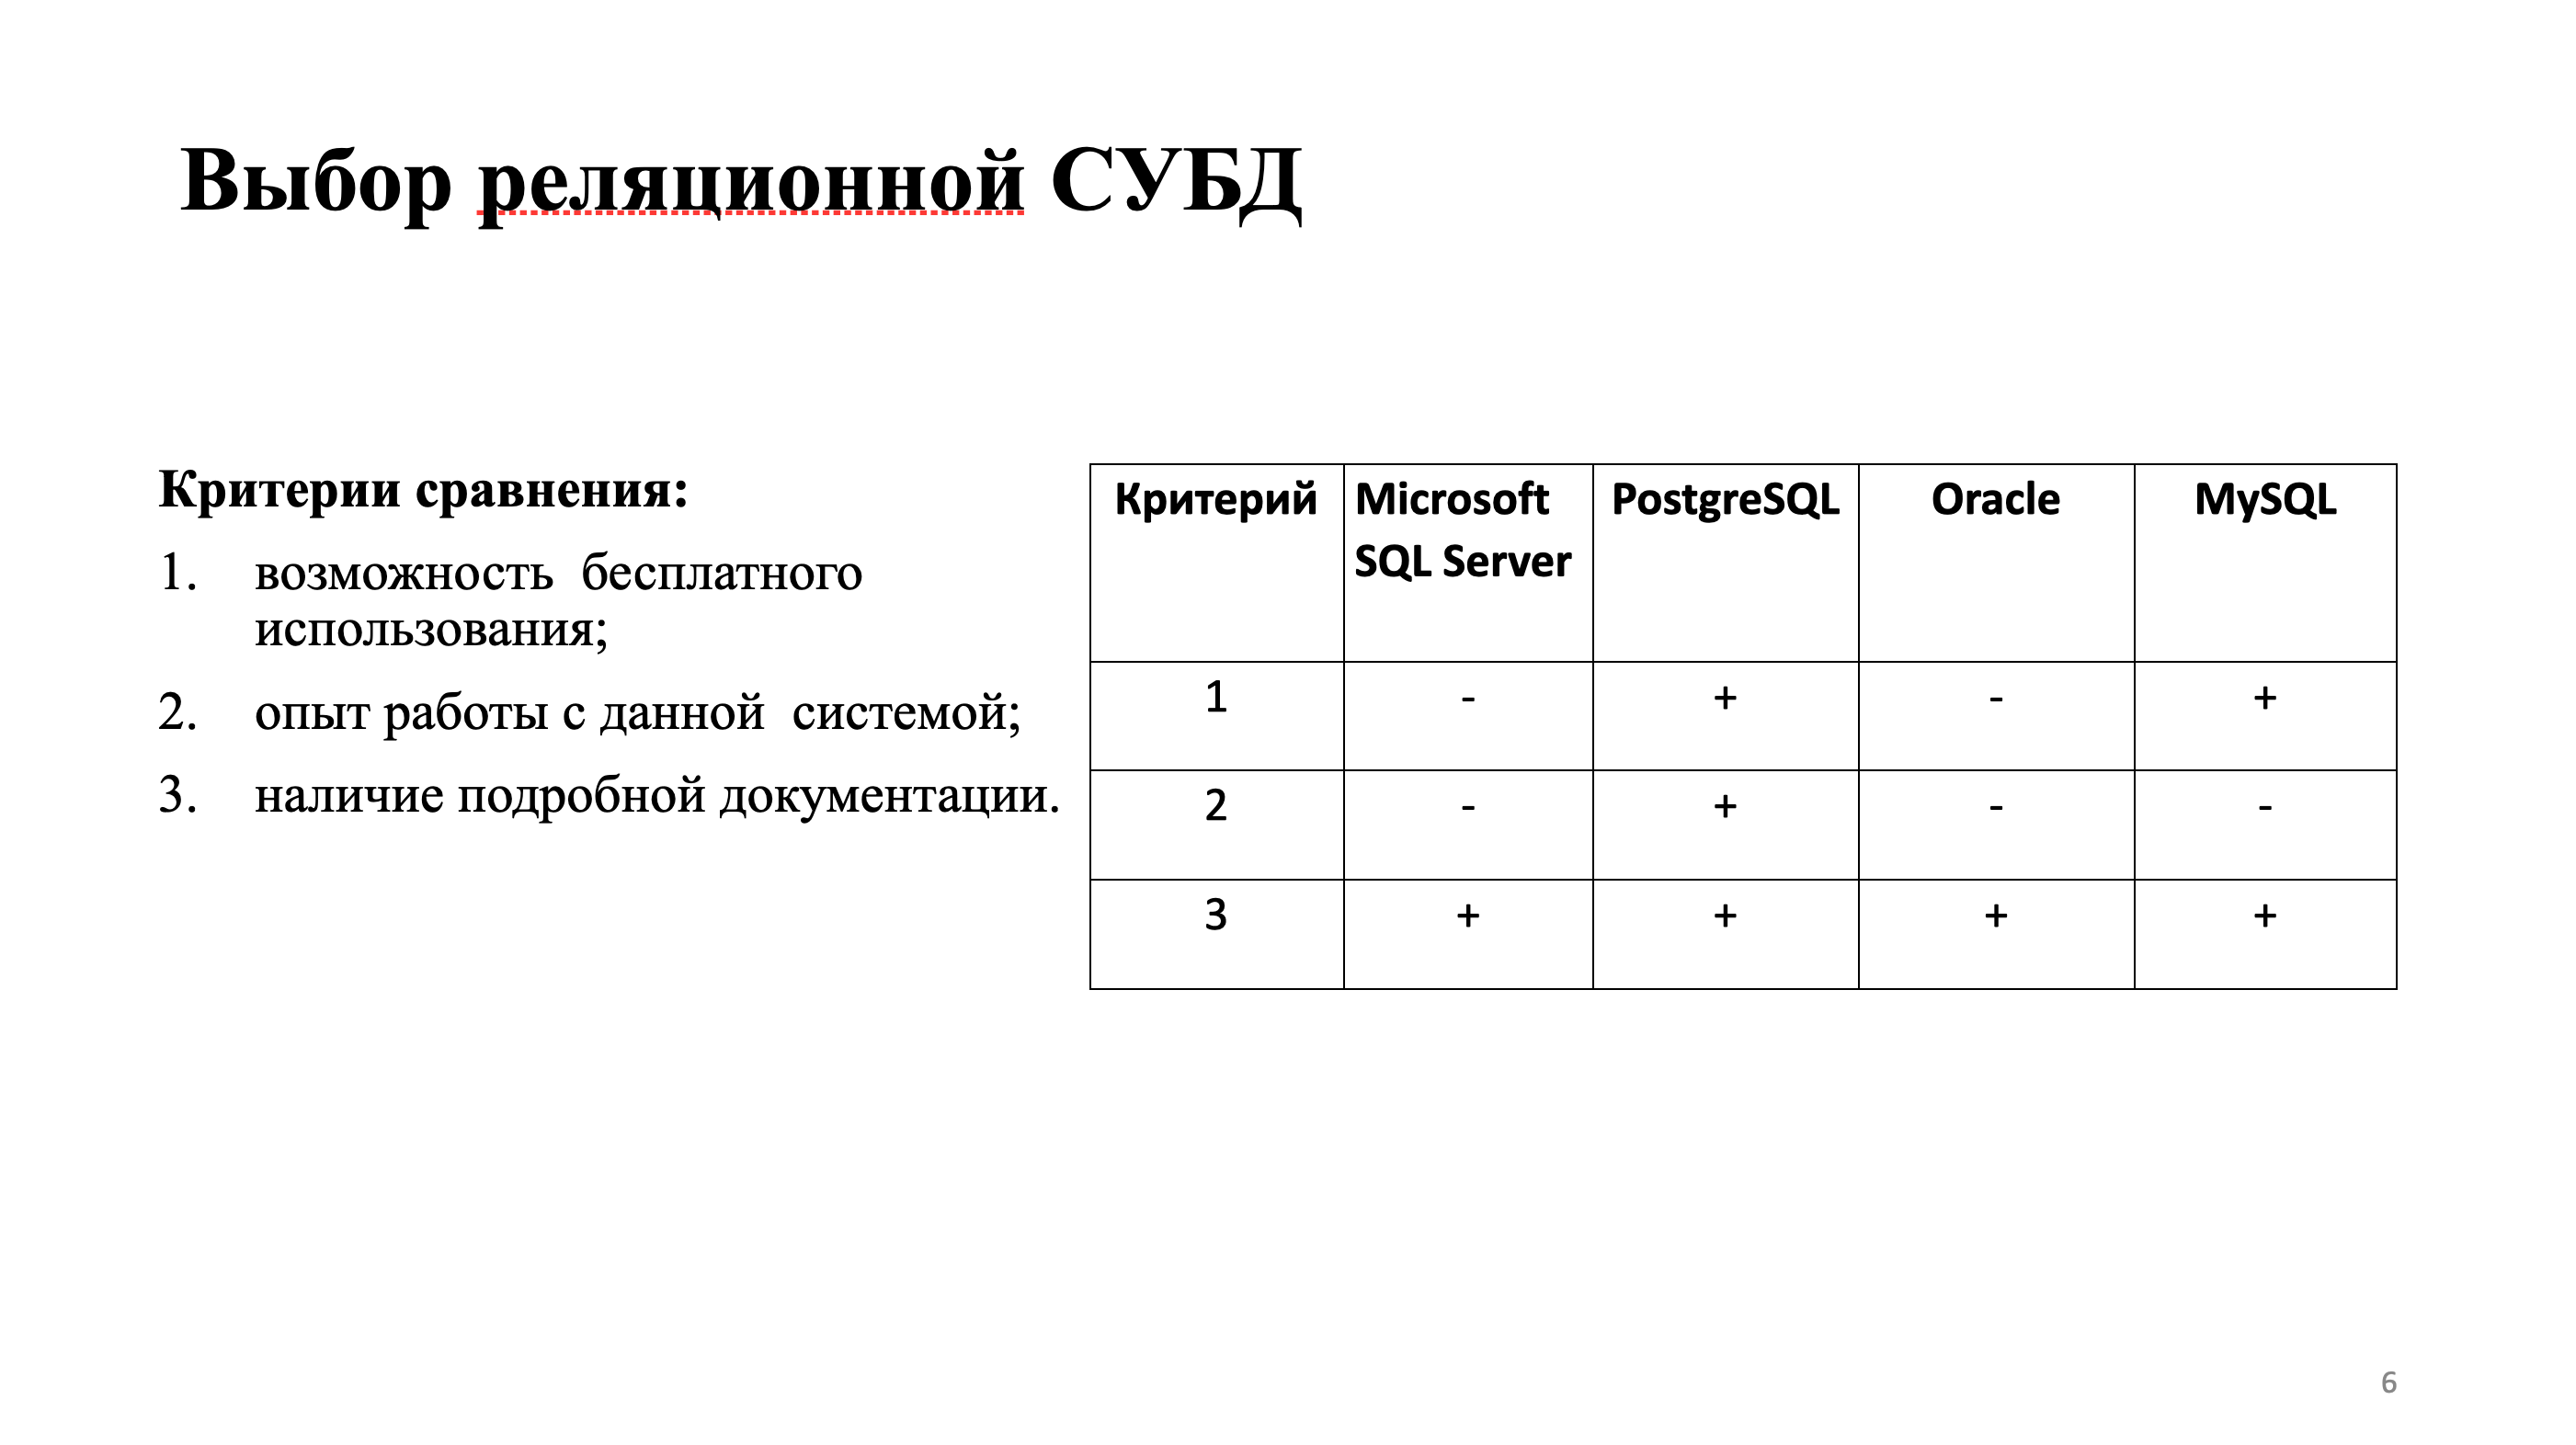
\includegraphics[width=1\linewidth]{img/6.png}
    \caption{Презентация -- слайд 6}
\end{figure}
\noindent

\begin{figure}[H]
    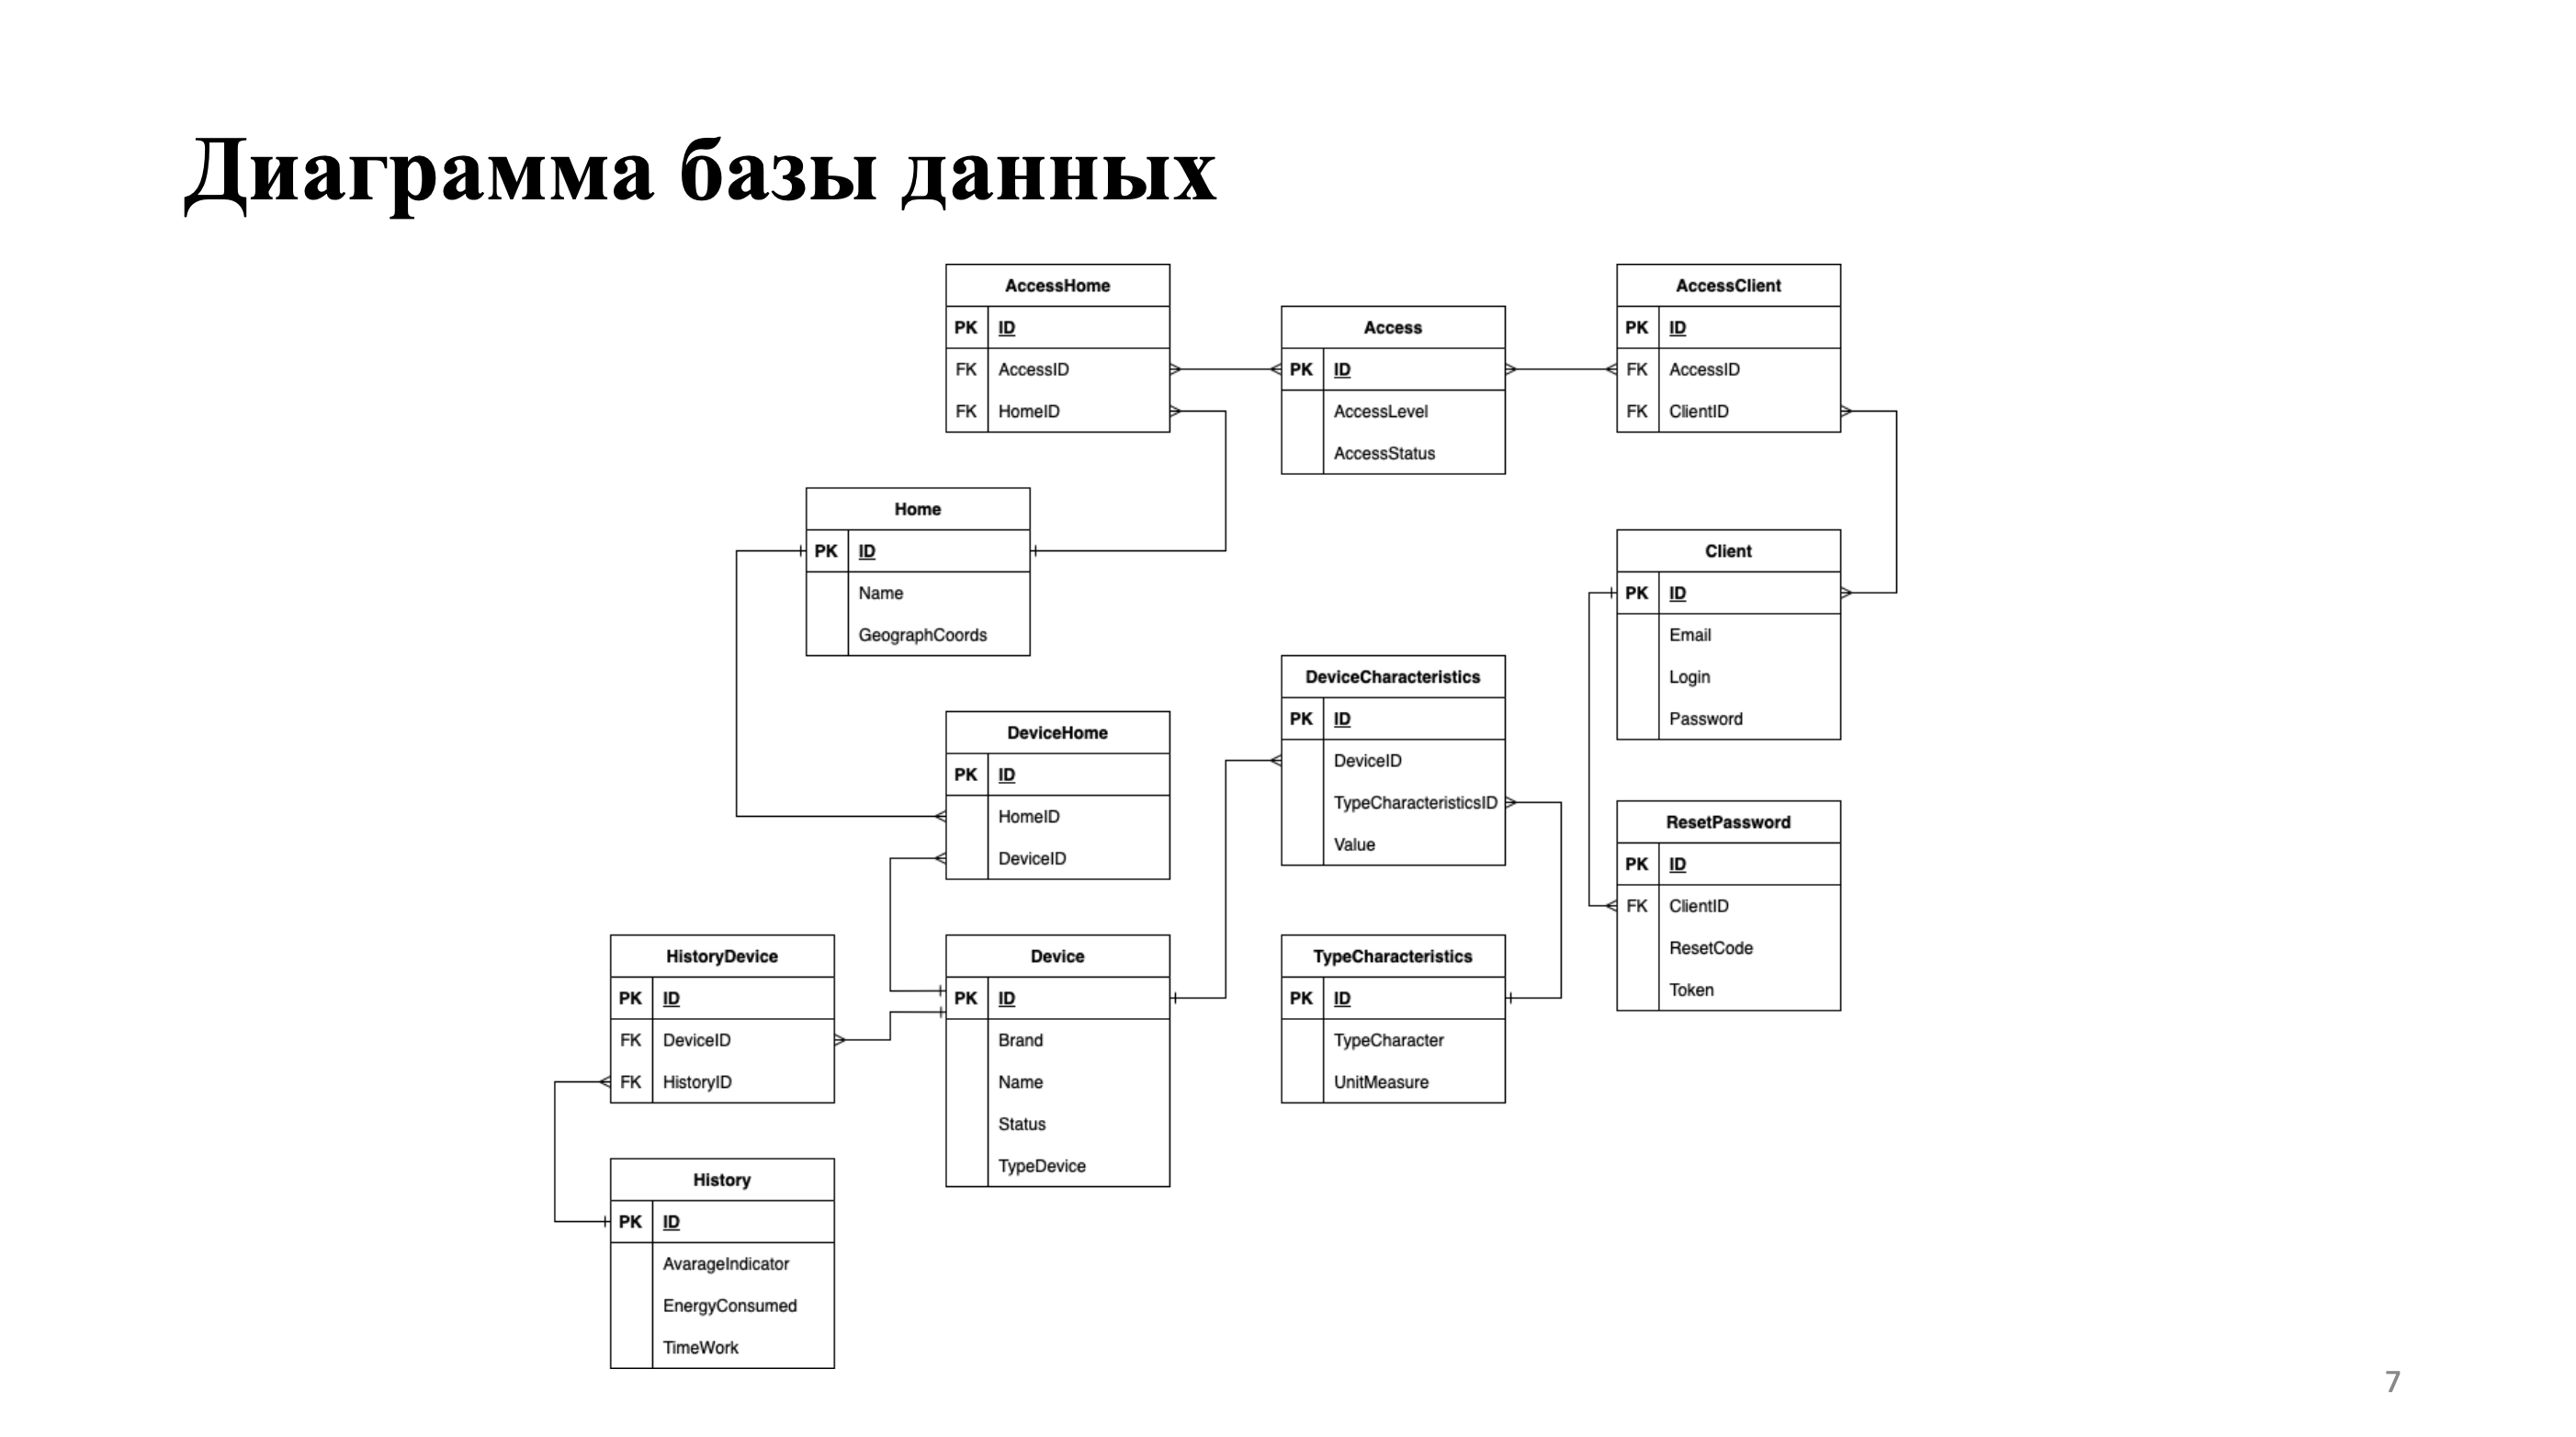
\includegraphics[width=1\linewidth]{img/7.png}
    \caption{Презентация -- слайд 7}
\end{figure}
\noindent

\begin{figure}[H]
    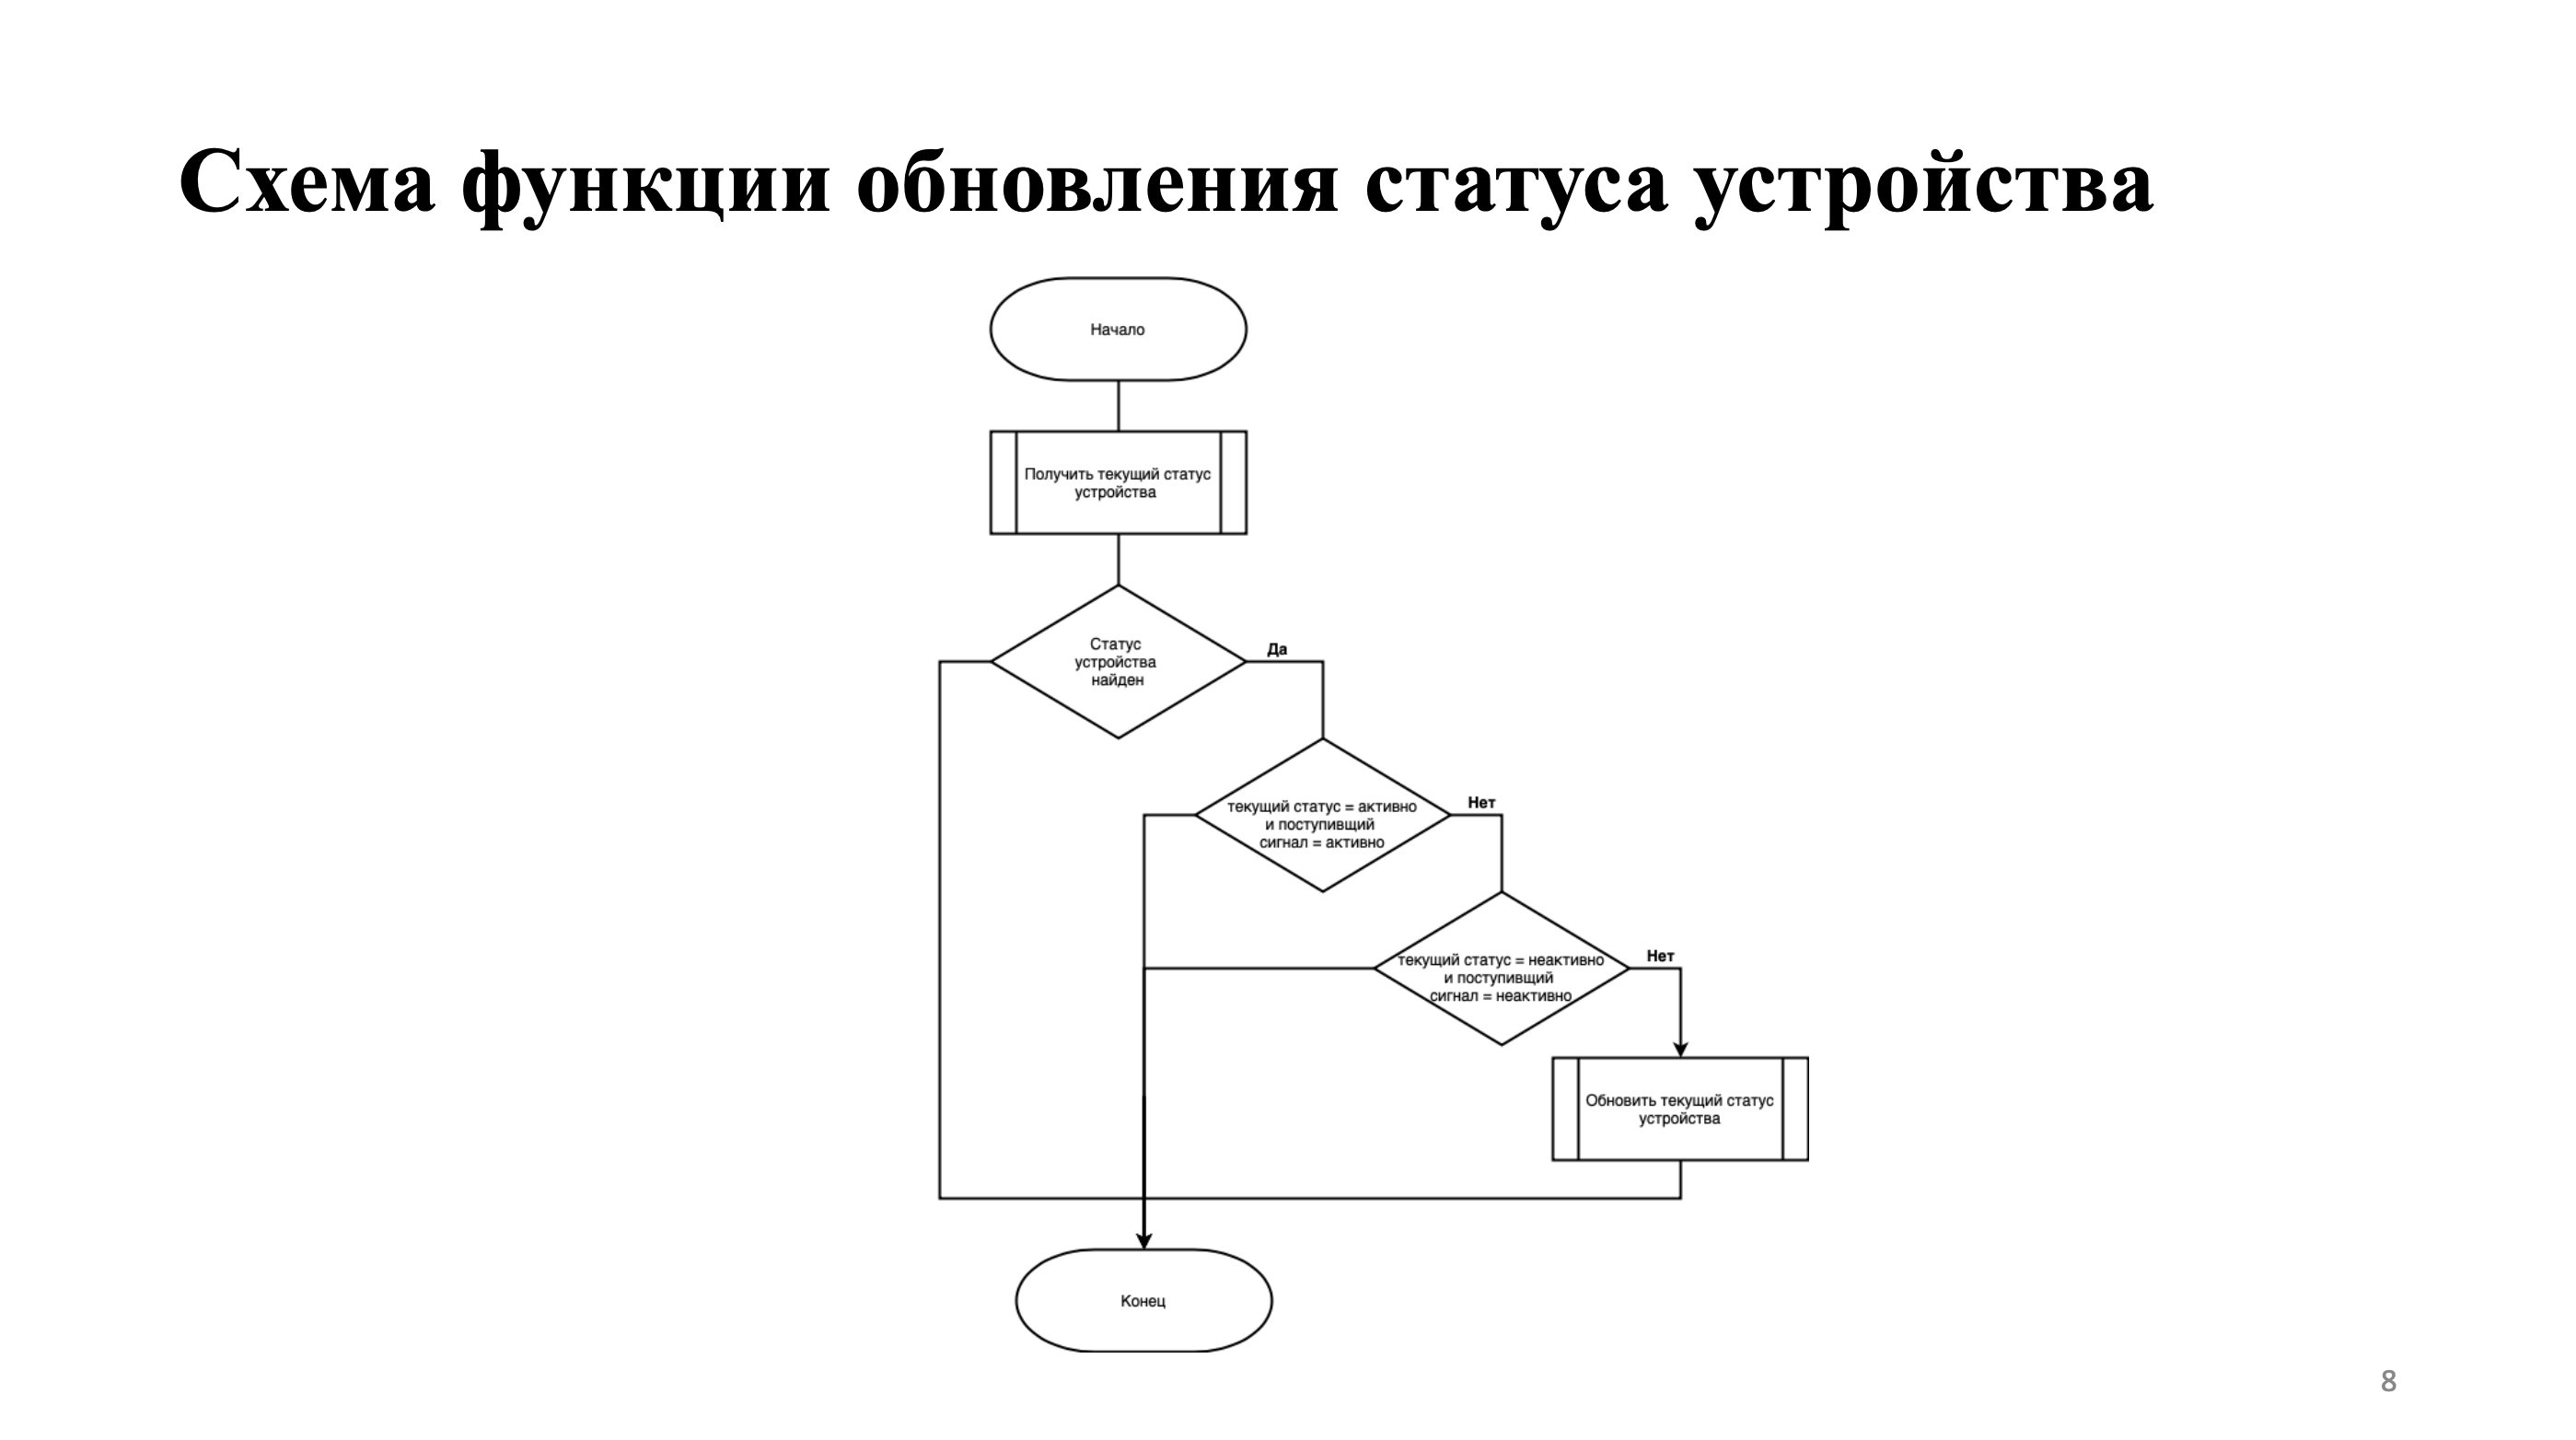
\includegraphics[width=1\linewidth]{img/8.png}
    \caption{Презентация -- слайд 8}
\end{figure}
\noindent

\begin{figure}[H]
    
\includegraphics[width=1\linewidth]{img/9.png}
    \caption{Презентация -- слайд 9}
\end{figure}
\noindent

\begin{figure}[H]
    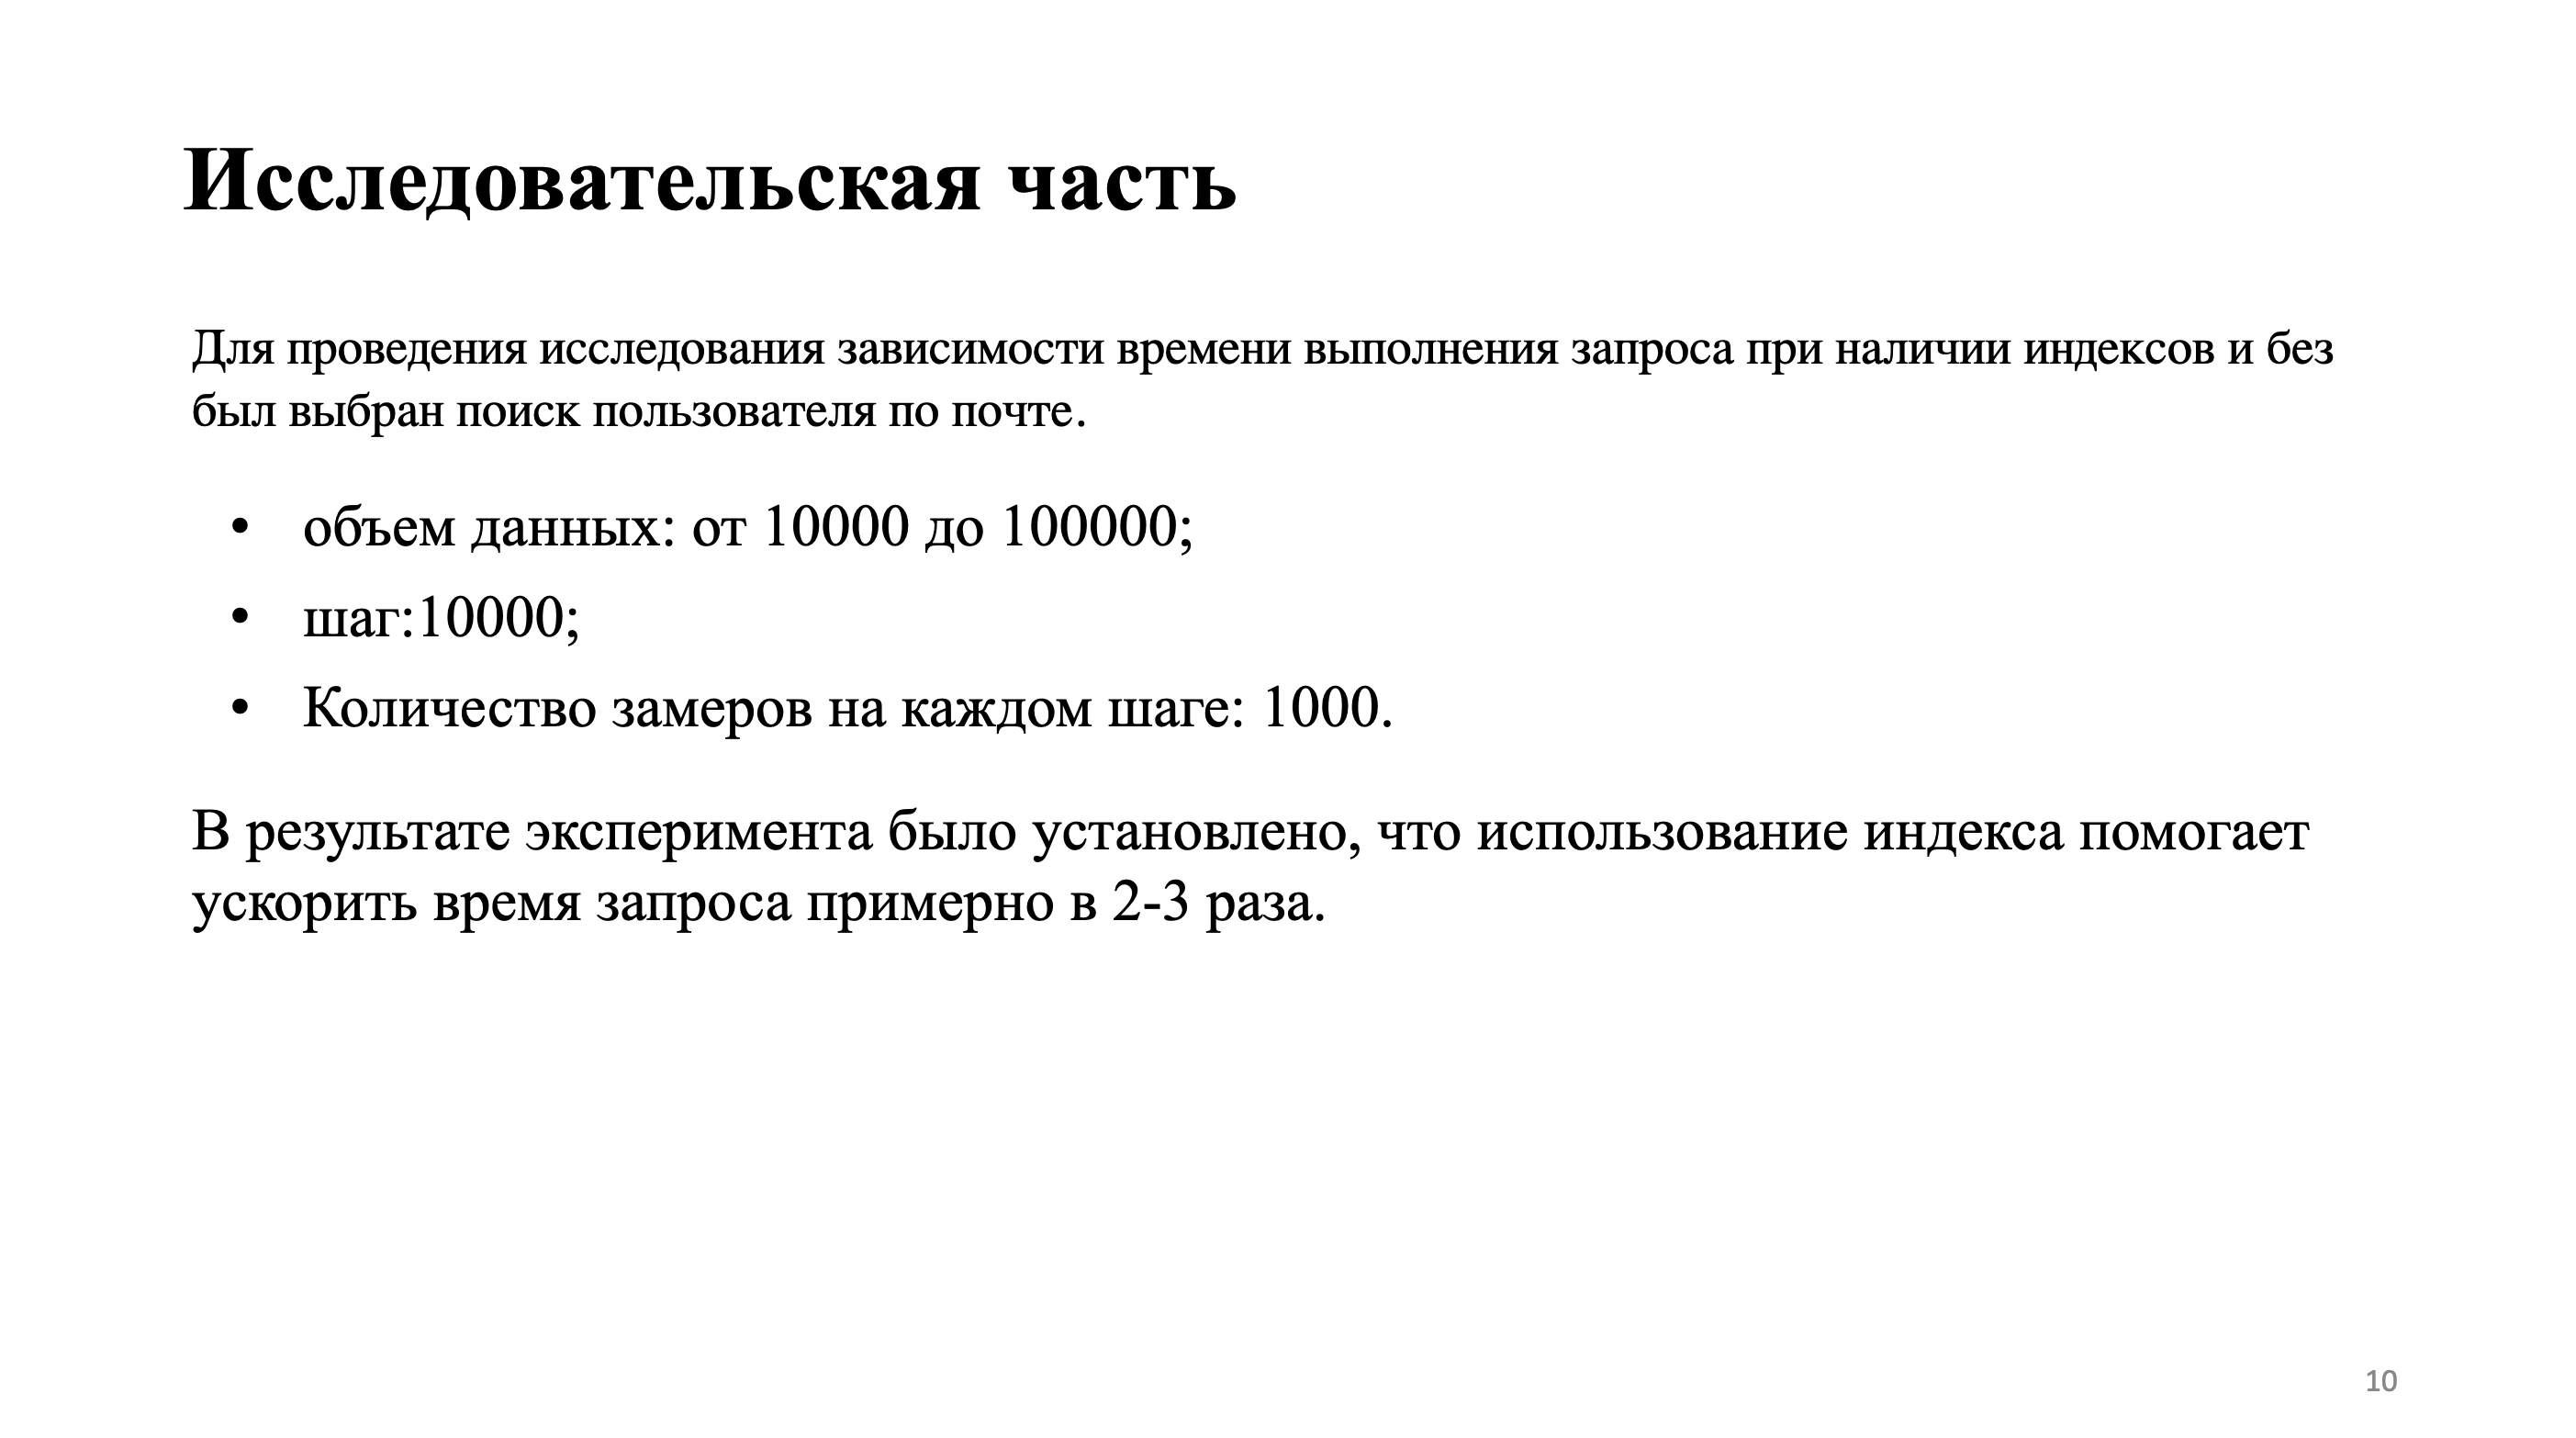
\includegraphics[width=1\linewidth]{img/10.png}
    \caption{Презентация -- слайд 10}
\end{figure}
\noindent

\begin{figure}[H]
    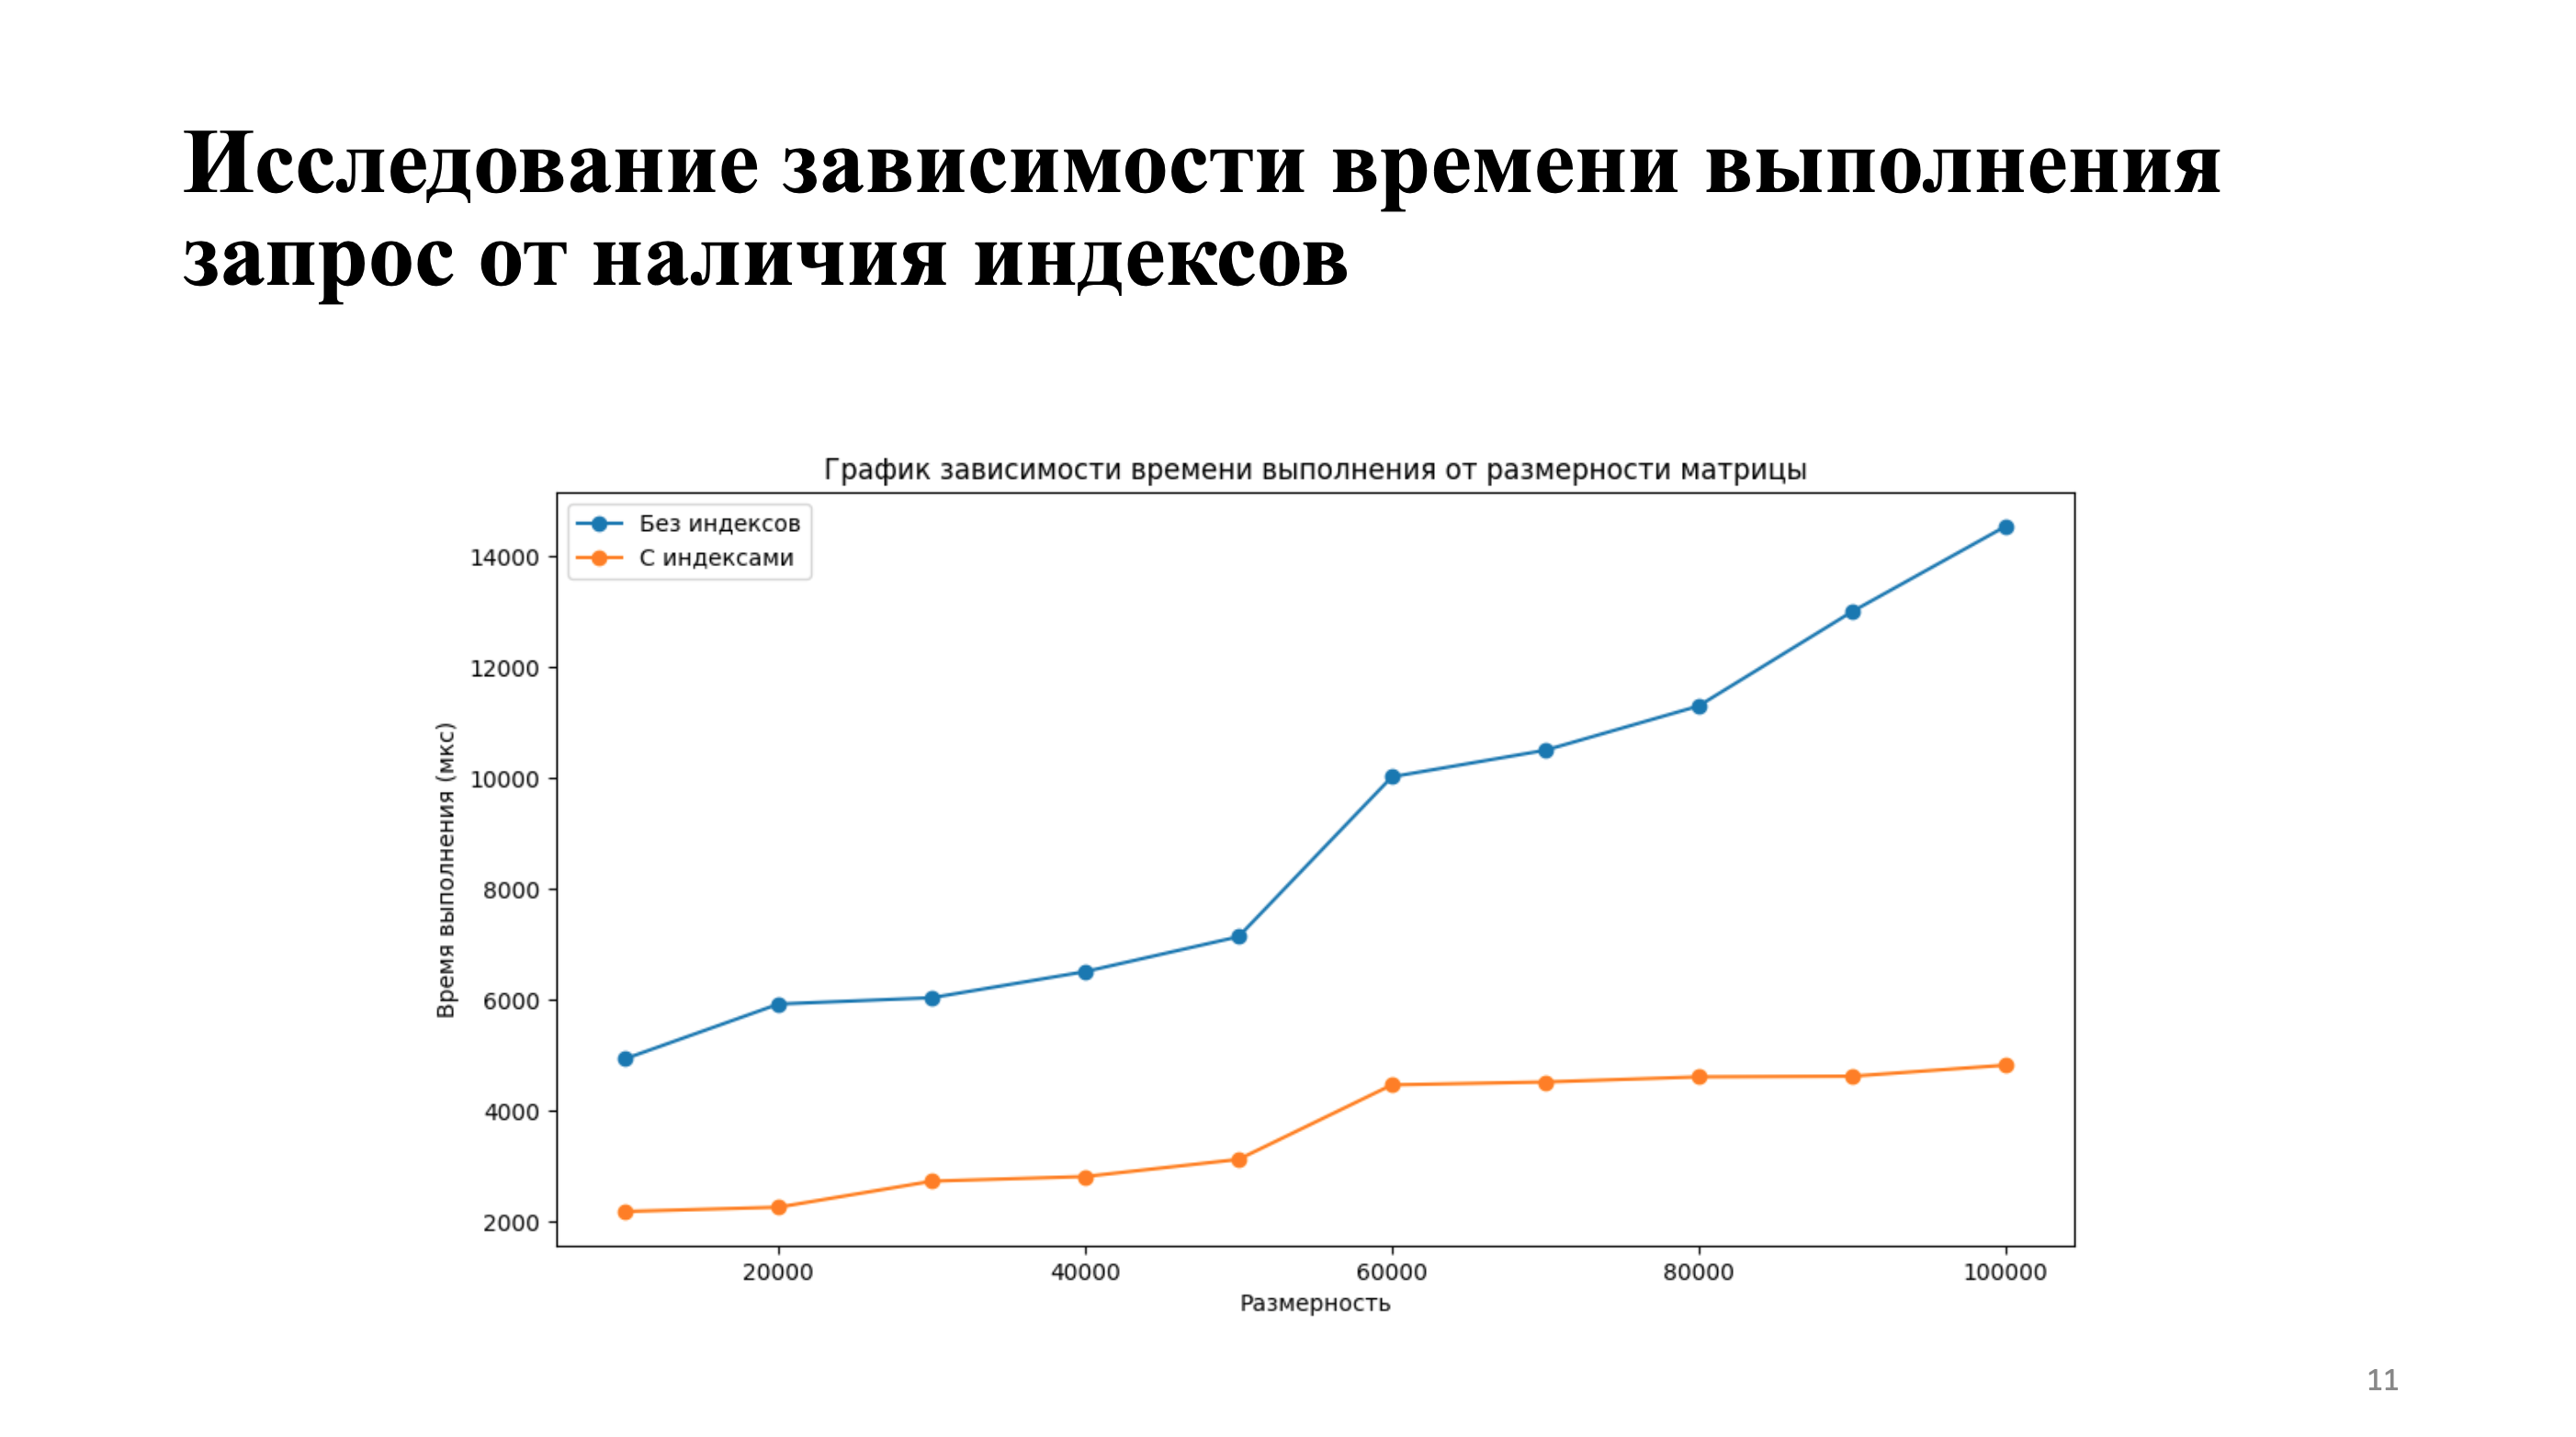
\includegraphics[width=1\linewidth]{img/11.png}
    \caption{Презентация -- слайд 11}
\end{figure}
\noindent

\begin{figure}[H]
    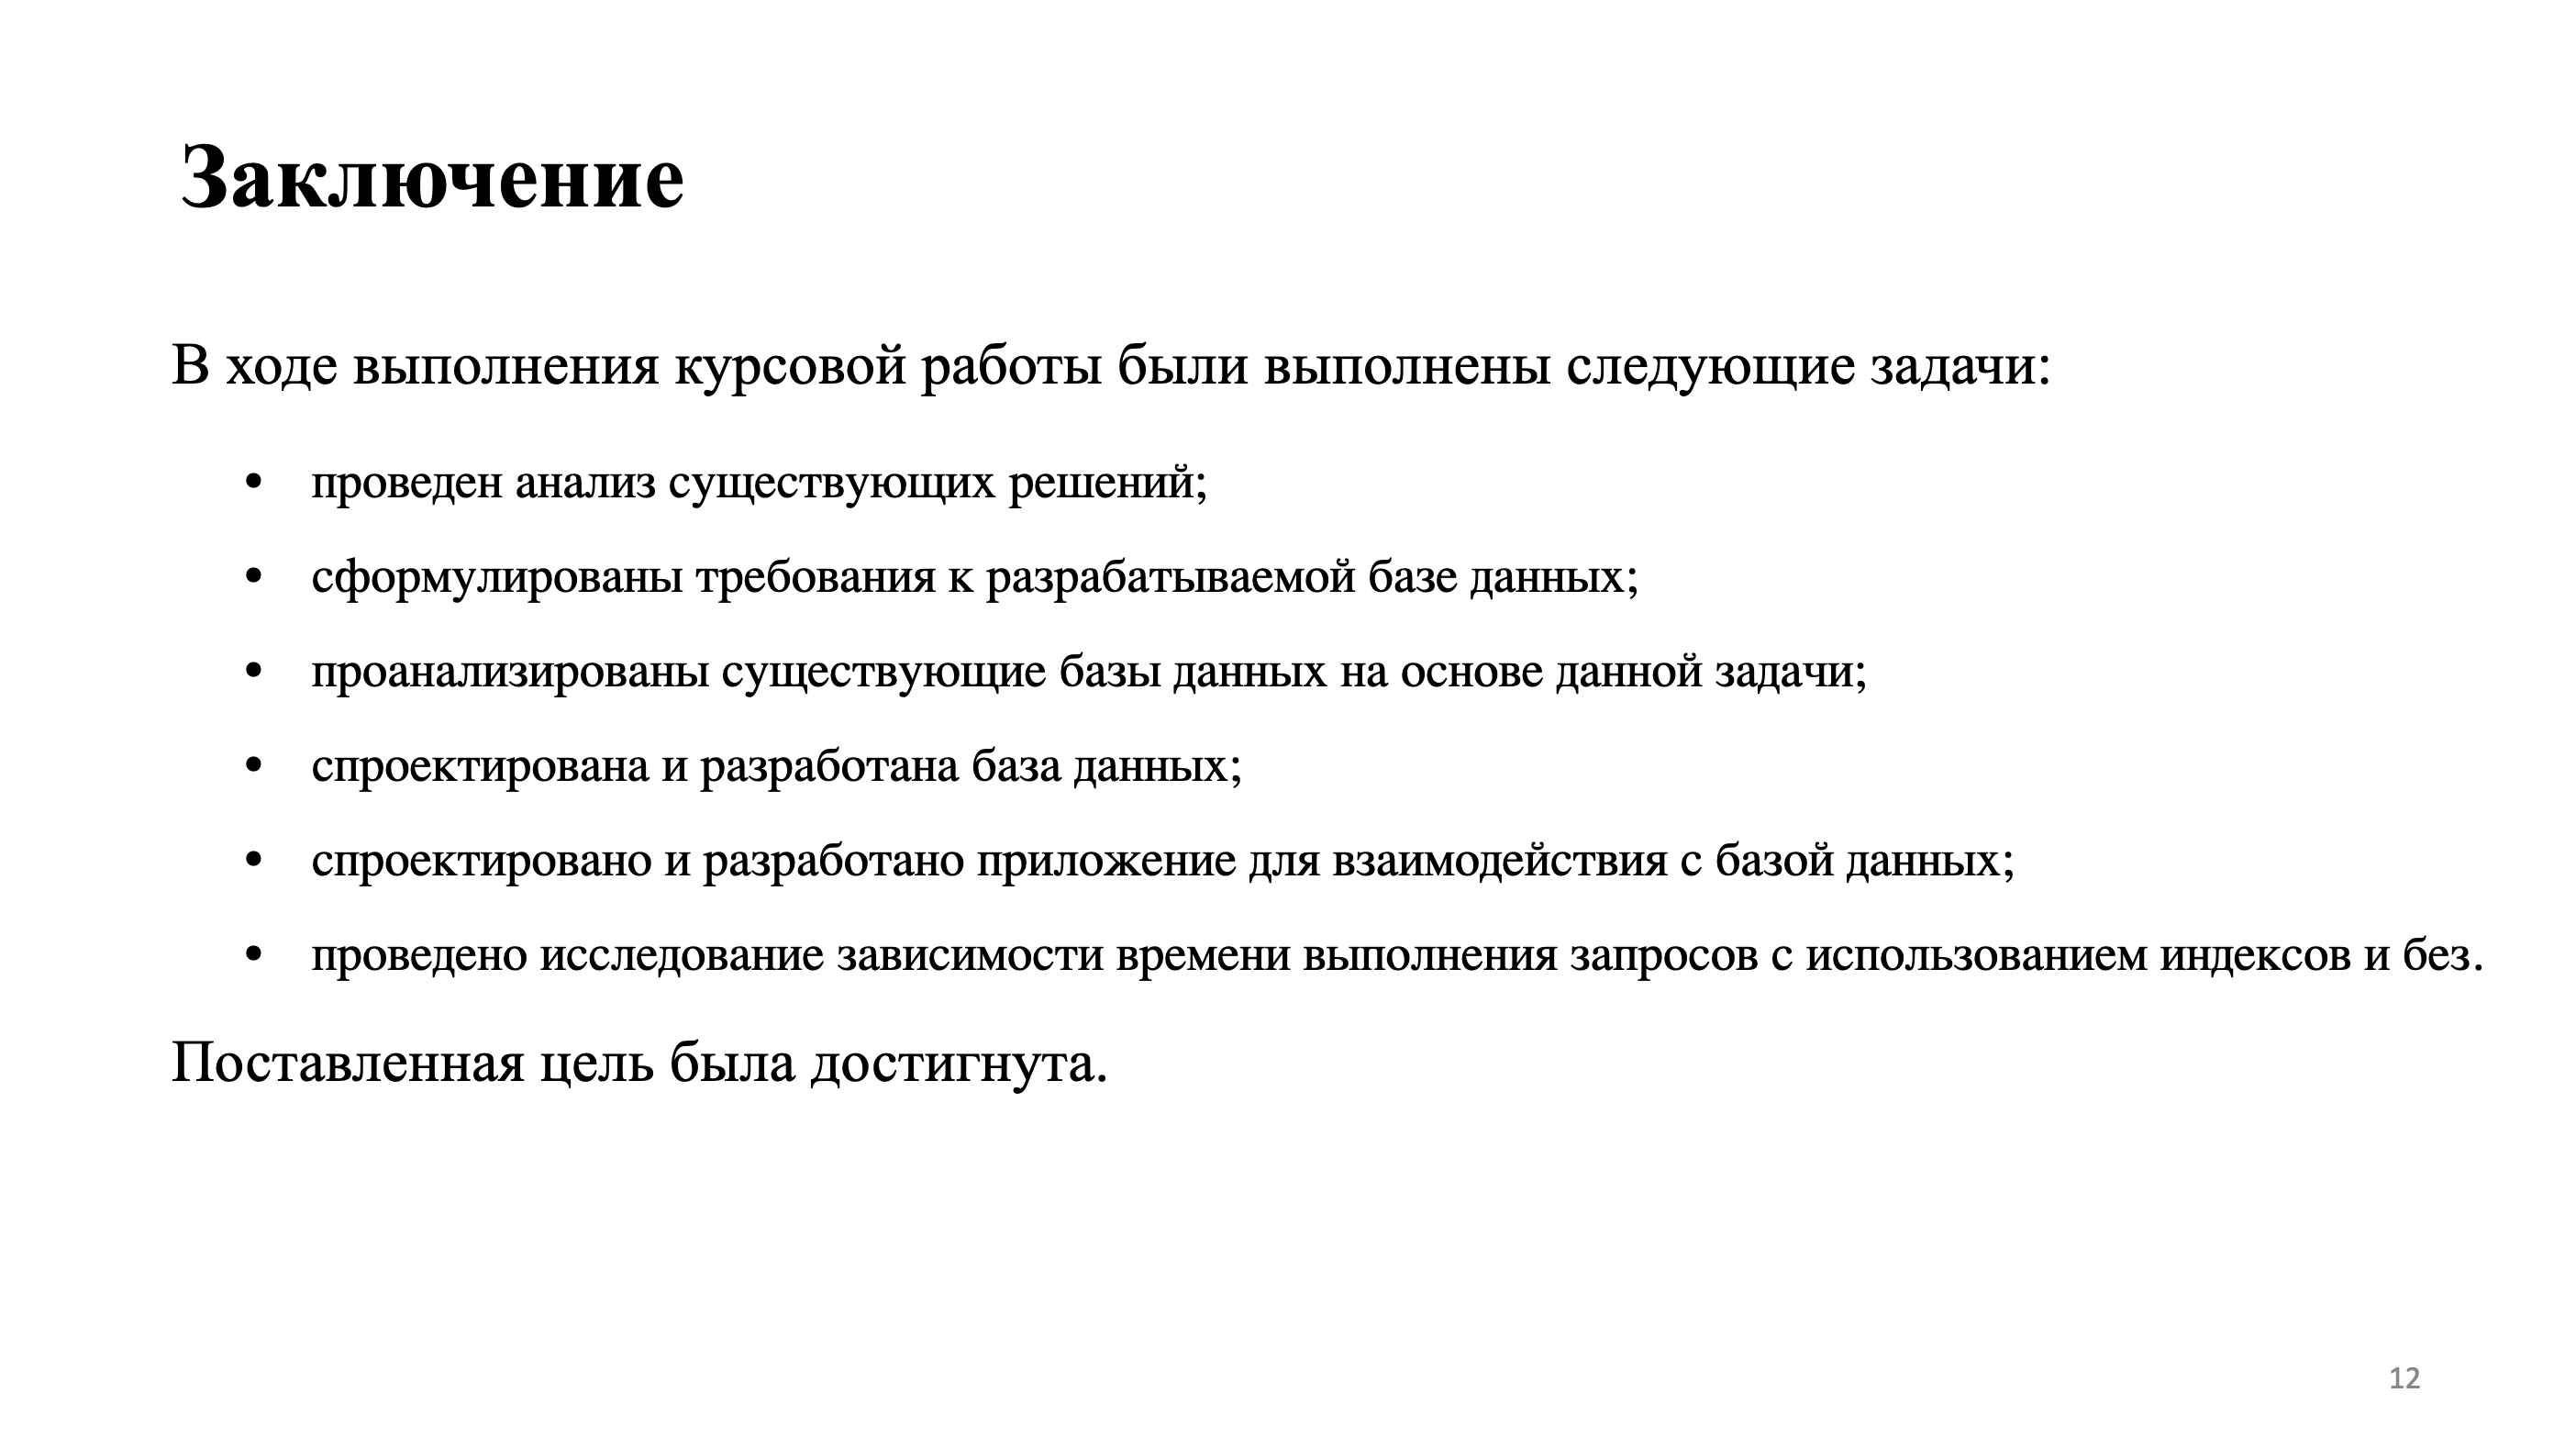
\includegraphics[width=1\linewidth]{img/12.png}
    \caption{Презентация -- слайд 12}
\end{figure}
\noindent

\end{document}
